% Trabalho de Política Urbana
%
% Abaixo seguem orientações originais do modelo utilizado
%
% ==============================================================
%
% Modelo para monografia de final de curso, em conformidade
% com normas da ABNT implementadas pelo projeto abntex2.
%
% Este arquivo é fortemente baseado em exemplo distribuído no
% mesmo projeto. O projeto abntex2 pode ser acessado pela página
% http://abntex2.googlecode.com/
%
% Este arquivo pode ser rodado tanto com o pdflatex quanto com
% o lualatex.  Como contém referências bibliográficas a serem
% processadas pelo programa bibtex, este programa deve ser
% executado. Em resumo, a ordem de execução deve ser:
% rodar primeiro o pdflatex (ou o lualatex), depois o bibtex e,
% a seguir, o pdflatex (ou o lualatex ) novamente mais duas vezes,
% para assegurar que todas as referências bibliográficas e 
% citações estejam atualizadas.
%
% Para adaptar os textos para uso pessoal, usar os comandos
% imediatamente antes do \begin{document} (iniciando com o
% comando \titulo).  
%
% Este modelo está adaptado para monografias de final de curso
% em matemática da UFRJ, mas, com o uso das variáveis, pode ser
% usado para outros tipos de trabalho (mestrado, doutorado),
% outros cursos, universidades etc.  Caso a adaptação das
% variáveis não seja suficiente, pode-se alterar os comandos
% imprimircapa, imprimirfolhaderosto e imprimiraprovação, 
% fazendo as alterações necessárias.  Como os comandos definidos
% neste texto usam somente LaTeX, a sua adaptação deve ser 
% simples, bastando algum conhecimento de LaTeX.
%
% O restante do preâmbulo provavelmente  não necessitará ser
% alterado, a menos, eventualmente, das opções de chamada da
% classe abntex2, que estão definidas a seguir.
% 
\documentclass[ 
% -- opções da classe memoir que é a classe base da abntex2 --
% tamanho da fonte
12pt,
% capítulos começam em pág ímpar. Insere pág vazia, se preciso
openright,
% para imprimir uma página por folha ou visualização em video 
oneside,
% frente e verso. Margens das pag. ímpares diferem das pares.
%  twoside,
% tamanho do papel. 
a4paper,
% Caio - Ocultando bordas horríveis em hiperligações
hidelinks,
% -- opções da classe abntex2 --
% títulos de capítulos convertidos em letras maiúsculas
%  chapter=TITLE,
% títulos de seções convertidos em letras maiúsculas
%  section=TITLE,
% títulos de subseções convertidos em letras maiúsculas
%  subsection=TITLE,
% títulos de subsubseções convertidos em letras maiúsculas
%  subsubsection=TITLE,
% -- opções do pacote babel --
english,   % idioma adicional para hifenização
portuguese,   % o último idioma é o principal do documento
oldfontcommands,
]{abntex2}
%
% ==============================================================
%
% --------------------------------------------------------------
% Adicionando pacotes para recursos adicionais e defindo opções
% pertinentes
% --------------------------------------------------------------
%
% cabeçalho comum para uso com lualatex ou pdflatex
\usepackage{ifluatex}
% opções para uso com o lualatex
\ifluatex
\usepackage{fontspec}
\defaultfontfeatures{Ligatures=TeX}
% o fonte small caps é diferente no latin modern
\fontspec[SmallCapsFont={Latin Modern Roman Caps}]{Latin Modern Roman}
% pacotes da AMS 
\usepackage{amsmath,amsthm} 
% pacote para fonte específico para símbolos matemáticos
\usepackage{unicode-math}
\setmathfont{Latin Modern Math}
% latin modern tem simbolos de mathbb muito feios.
%  Trocar o fonte para estes simbolos.
\setmathfont[range=\mathbb]{Tex Gyre Pagella Math}
% opções para uso com o pdflatex
\else
\usepackage[utf8x]{inputenc}
\usepackage[T1]{fontenc}
\usepackage{lmodern}
\usepackage{etoolbox}
% pacotes da AMS 
\usepackage{amsmath,amssymb,amsthm} 
% Mapear caracteres especiais no PDF
\usepackage{cmap}
\fi

% pacotes usados tanto pelo lualatex quanto pelo pdflatex
\usepackage{lastpage}    % Usado pela Ficha catalográfica
\usepackage{indentfirst} % Indenta primeiro parágrafo 
\usepackage{color}       % Controle das cores
\usepackage{graphicx}    % Inclusão de gráficos
\usepackage{wrapfig}     % gráficos ao redor do texto
% pacote para ajustar os fontes em cada linha de forma a
% respeitar as margens
\usepackage{microtype}
% permite a gravação de texto em um arquivo indicado a partir
% deste arquivo.  Originalmente foi usado para criar o arquivo
% .bib com conteúdo de exemplo, evitando a edição de um arquivo
% .bib somente para a bibliografia
\usepackage{filecontents}

% Caio - diagramas
% http://www.texample.net/tikz/examples/smart-priority/
%\usepackage{smartdiagram}

% Caio - ladeando imagens
% https://tex.stackexchange.com/questions/57433/cannot-use-caption-under-minipage
\usepackage{caption}

% Caio - preciso de tabelas longas
% http://www.tex.ac.uk/FAQ-figurehere.html
\usepackage{longtable}

% Caio - tentando melhorar o posicionamento das imagens
\usepackage{float}

% Caio - corrigindo espaçamento conforme http://tex.stackexchange.com/questions/5683/how-to-remove-top-and-bottom-whitespace-of-longtable
\setlength{\LTpre}{0pt}
\setlength{\LTpost}{0pt}

% Caio - preciso de plotagens
%\usepackage{pgfplots}
%\pgfplotsset{compat=1.8}

% Caio - quero usar letras nas listas do enumerate conforme https://tex.stackexchange.com/questions/2291/how-do-i-change-the-enumerate-list-format-to-use-letters-instead-of-the-defaul
\usepackage{enumitem}

% Caio - modo paisagem para tabelões
\usepackage{lscape}

% Caio - adicionando o pacote hyperref
\usepackage{hyperref}
% - e definindo metadados do PDF e comportamento dos links
\hypersetup{
	%pagebackref=true,
	pdftitle={Relatório/Diagnóstico de Política Urbana}, 
	pdfauthor={Anderson, Caio, Jade, Henrique, Noele},
	pdfsubject={Política Urbana},
	colorlinks=false,      		% false: boxed links; true: colored links
	linkcolor=blue,          	% color of internal links
	citecolor=blue,        		% color of links to bibliography
	filecolor=magenta,      	% color of file links
	urlcolor=blue,
	bookmarksdepth=4
}

% Caio - separação silábica
%\hyphenation{}

% Caio - citações mais poderosas
%\usepackage[autostyle]{csquotes}

%-----------------------------------------------------------
%-----------------------------------------------------------
% Caio - habilitar glossário
\usepackage{glossaries}
\makeglossaries

% \newglossaryentry{ex}{name={sample},description={an example}}
\newglossaryentry{abl}{
	name={ABL},
	description={Área Bruta Locável}
}

\newglossaryentry{auj}{
	name={AUJ},
	description={Aglomeração Urbana de Jundiaí}
}

\newglossaryentry{condephaat}{
	name={CONDEPHAAT},
	description={Conselho de Defesa do Patrimônio Histórico, Arqueológico, Artístico e Turístico}
}

\newglossaryentry{cptm}{
	name={CPTM},
	description={Companhia Paulista de Trens Metropolitanos}
}

\newglossaryentry{tim}{
	name={TIM},
	description={Trem Intra-Metropolitano}
}

\newglossaryentry{cmsp}{
	name={CMSP},
	description={Companhia do Metropolitano de São Paulo}
}

\newglossaryentry{embraesp}{
	name={Embraesp},
	description={Empresa Brasileira de Estudos de Patrimônio}
}

\newglossaryentry{emtu}{
	name={EMTU},
	description={Empresa Metropolitana de Transportes Urbanos de São Paulo S.A}
}

\newglossaryentry{emplasa}{
	name={Emplasa},
	description={Empresa Paulista de Planejamento Metropolitano S/A}
}

\newglossaryentry{luos}{
	name={LUOS},
	description={Lei de Uso de Ocupação do Solo}
}

\newglossaryentry{mdu}{
	name={MDU},
	description={Média por Dia Útil}
}

\newglossaryentry{ouc}{
	name={OUC},
	description={Operação Urbana Consorciada}
}

\newglossaryentry{pde}{
	name={PDE},
	description={Plano Diretor Estratégico}
}

\newglossaryentry{peuc}{name={PEUC},description={Parcelamento, Edificação e Utilização Compulsórios}}

\newglossaryentry{pl}{
	name={PL},
	description={Projeto de Lei}
}

\newglossaryentry{rmsp}{
	name={RMSP},
	description={Região Metropolitana de São Paulo}
}

\newglossaryentry{rmbs}{
	name={RMBS},
	description={Região Metropolitana da Baixada Santista}
}

\newglossaryentry{cetesb}{
	name={Cetesb},
	description={Companhia Ambiental do Estado de São Paulo}
}

\newglossaryentry{sapavel}{
	name={SAPAVEL},
	description={Sistema de Áreas Protegidas, Áreas Verdes e Espaços Livres}
}

\newglossaryentry{smdu}{
	name={SMDU},
	description={Secretaria Municipal de Desenvolvimento Urbano da Prefeitura de São Paulo}
}

\newglossaryentry{idhm}{
	name={IDHM},
	description={Índice de Desenvolvimento Humano}
}

\newglossaryentry{efs}{
	name={EFS},
	description={Estrada de Ferro Sorocabana}
}

\newglossaryentry{vlt}{
	name={VLT},
	description={Veículo Leve sobre Trilhos}
}

\newglossaryentry{brt}{
	name={BRT},
	description={Bus Rapid Transit}
}

\newglossaryentry{rffsa}{
	name={RFFSA},
	description={Rede Ferroviária Federal Sociedade Anônima}
}

\newglossaryentry{iptu}{
	name={IPTU},
	description={Imposto Predial e Territorial Urbano}
}

\newglossaryentry{fepasa}{
	name={Fepasa},
	description={Ferrovia Paulista Sociedade Anônima}
}

\newglossaryentry{iss}{
	name={ISS},
	description={Imposto Sobre Serviços de Qualquer Natureza}
}

\newglossaryentry{app}{
	name={APP},
	description={Área de Preservação Permanente}
}

\newglossaryentry{luops}{
	name={LUOPS},
	description={Legislação de Ordenamento do Uso, da Ocupação e do Parcelamento do Solo}
}

\newglossaryentry{plhis}{
	name={PLHIS},
	description={Plano Local de Habitação de Interesse Social}
}

\newglossaryentry{sabesp}{
	name={Sabesp},
	description={Companhia de Saneamento Básico do Estado de São Paulo}
}

\newglossaryentry{pddmap}{
	name={PDDMAP},
	description={Plano Diretor de Drenagem e Manejo de Águas Pluviais}
}

\newglossaryentry{agem}{
	name={AGEMBS},
	description={Agência Metropolitana da Baixada Santista}
}

\newglossaryentry{pac}{
	name={PAC},
	description={Programa de Aceleração do Crescimento}
}

\newglossaryentry{zeis}{
	name={ZEIS},
	description={Zona Especial de Interesse Social}
}

\newglossaryentry{ac1}{
	name={AC-1},
	description={Clubes esportivos sociais}
}

\newglossaryentry{ac2}{
	name={AC-2},
	description={Clubes de campo e clubes náuticos}
}

\newglossaryentry{zc}{
	name={ZC},
	description={Zona Centralidade}
}

\newglossaryentry{zczeis}{
	name={ZC-ZEIS},
	description={Zona Centralidade lindeira à ZEIS}
}

\newglossaryentry{zca}{
	name={ZCa},
	description={Zona Centralidade Ambiental}
}

\newglossaryentry{zcor1}{
	name={ZCOR-1},
	description={Zona Corredor 1}
}

\newglossaryentry{zcor2}{
	name={ZCOR-2},
	description={Zona Corredor 2}
}

\newglossaryentry{zcor3}{
	name={ZCOR-3},
	description={Zona Corredor 3}
}

\newglossaryentry{zcora}{
	name={ZCORa},
	description={Zona Corredor Ambiental}
}

\newglossaryentry{zde1}{
	name={ZDE-1},
	description={Zona de Desenvolvimento Econômico 1}
}

\newglossaryentry{zde2}{
	name={ZDE-2},
	description={Zona de Desenvolvimento Econômico 2}
}

\newglossaryentry{zeis1}{
	name={ZEIS-1},
	description={Zona Especial de Interesse Social 1}
}

\newglossaryentry{zeis2}{
	name={ZEIS-2},
	description={Zona Especial de Interesse Social 2}
}

\newglossaryentry{zeis3}{
	name={ZEIS-3},
	description={Zona Especial de Interesse Social 3}
}

\newglossaryentry{zeis4}{
	name={ZEIS-4},
	description={Zona Especial de Interesse Social 4}
}

\newglossaryentry{zeis5}{
	name={ZEIS-5},
	description={Zona Especial de Interesse Social 5}
}

\newglossaryentry{zem}{
	name={ZEM},
	description={Zona Eixo de Estruturação Transformação Metropolitana}
}

\newglossaryentry{zemp}{
	name={ZEMP},
	description={Zona Eixo de Estruturação Transformação Metropolitana Previsto}
}

\newglossaryentry{zep}{
	name={ZEP},
	description={Zona Especial de Preservação}
}

\newglossaryentry{zepam}{
	name={ZEPAM},
	description={Zona Especial de Proteção Ambiental}
}

\newglossaryentry{zer1}{
	name={ZER-1},
	description={Zona Exclusivamente Residencial 1}
}

\newglossaryentry{zer2}{
	name={ZER-2},
	description={Zona Exclusivamente Residencial 2}
}

\newglossaryentry{zera}{
	name={ZERa},
	description={Zona Exclusivamente Residencial Ambiental}
}

\newglossaryentry{zeu}{
	name={ZEU},
	description={Zona Eixo de Estruturação da Transformação Urbana}
}

\newglossaryentry{zeua}{
	name={ZEUa},
	description={Zona Eixo de Estruturação da Transformação Urbana Ambiental}
}

\newglossaryentry{zeup}{
	name={ZEUP},
	description={Zona Eixo de Estruturação da Transformação Previsto}
}

\newglossaryentry{zeupa}{
	name={ZEUPa},
	description={Zona Eixo de Estruturação da Transformação Previsto Ambiental}
}

\newglossaryentry{zm}{
	name={ZM},
	description={Zona Mista}
}

\newglossaryentry{zma}{
	name={ZMa},
	description={Zona Mista Ambiental}
}

\newglossaryentry{zmis}{
	name={ZMIS},
	description={Zona Mista de Interesse Social}
}

\newglossaryentry{zmisa}{
	name={ZMISa},
	description={Zona Mista de Interesse Social Ambiental}
}

\newglossaryentry{zoe}{
	name={ZOE},
	description={Zona de Ocupação Especial}
}

\newglossaryentry{zpds}{
	name={ZPDS},
	description={Zona de Preservação e Desenvolvimento Sustentável}
}

\newglossaryentry{zpdsr}{
	name={ZPDSr},
	description={Zona de Preservação e Desenvolvimento Sustentável da Zona Rural}
}

\newglossaryentry{zpi1}{
	name={ZPI-1},
	description={Zona Predominantemente Industrial 1}
}

\newglossaryentry{zpi2}{
	name={ZPI-2},
	description={Zona Predominantemente Industrial 1}
}

\newglossaryentry{zpr}{
	name={ZPR},
	description={Zona Predominantemente Residencial}
}

\newglossaryentry{pmsp}{
	name={PMSP},
	description={Prefeitura do Município de São Paulo}
}

\newglossaryentry{smpr}{
	name={SMPR},
	description={Secretaria Municipal de Prefeituras Regionais}
}

\newglossaryentry{smg}{
	name={SMG},
	description={Secretaria Municipal de Gestão}
}

\newglossaryentry{ibge}{
	name={IBGE},
	description={Instituto Brasileiro de Geografia e Estatística}
}

\newglossaryentry{gesp}{
	name={GESP},
	description={Governo do Estado de São Paulo}
}

%-----------------------------------------------------------
%-----------------------------------------------------------
% Comandos para definir ambientes tipo teorema em português 
\newtheorem{meuteorema}{Teorema}[chapter]
\newtheorem{meuaxioma}{Axioma}[chapter]
\newtheorem{meucorolario}{Corolário}[chapter]
\newtheorem{meulema}{Lema}[chapter]
\newtheorem{minhaproposicao}{Proposição}[chapter]
\newtheorem{minhadefinicao}{Definição}[chapter]
\newtheorem{meuexemplo}{Exemplo}[chapter]
\newtheorem{minhaobservacao}{Observação}[chapter]
%-----------------------------------------------------------
%-----------------------------------------------------------
% Pacotes de citações
\usepackage[brazilian,hyperpageref]{backref}
\usepackage[alf]{abntex2cite}   % Citações padrão ABNT
%\usepackage[num]{abntex2cite}  % Citações numéricas
% --- 
% Configurações do pacote backref
% Usado sem a opção hyperpageref de backref
\renewcommand{\backrefpagesname}{Citado na(s) página(s):~}
% Texto padrão antes do número das páginas
\renewcommand{\backref}{}
% Define os textos da citação
\renewcommand*{\backrefalt}[4]{
	\ifcase #1 %
	Nenhuma citação no texto.%
	\or
	Citado na página #2.%
	\else
	Citado #1 vezes nas páginas #2.%
	\fi}%
% --- 
% --- 
% Espaço em branco no início do parágrafo
\setlength{\parindent}{1.3cm}
% Controle do espaçamento entre um parágrafo e outro:
\setlength{\parskip}{0.2cm}  % tente também \onelineskip
% ---
% compila o indice, se este for incluído no texto
\makeindex
%
% --------------------------------------------------------- 
% ---------------------------------------------------------
% Redefinindo o comando do abntex2 para gerar uma capa  
\renewcommand{\imprimircapa}{%
	\begin{capa}
	\begin{flushleft} 
		{\Large \textsc{\imprimirinstituicao  \\
				\imprimircurso \\} }
	\end{flushleft}
	
	\vfill
	\begin{center}
		{\large \imprimirautor} \\
		{\Large \textit{\imprimirtitulo}}
	\end{center}
	
	\vfill
	\begin{center}
		{\large{\imprimirlocal \\ \imprimirano  }}
	\end{center}
	\vspace*{1cm} 
	\end{capa}
	
}

% ---------------------------------------------------------
% ---------------------------------------------------------
%
%
% ---------------------------------------------------------
% ---------------------------------------------------------
% Redefinindo o comando para gerar uma folha de rosto 
\renewcommand{\imprimirfolhaderosto}{%
	\begin{center}
		{\large \imprimirautor}
	\end{center}
	\vfill \vfill \vfill \vfill
	\begin{center}
		{\Large \textit{\imprimirtitulo}}
	\end{center}
	
	\vfill \vfill \vfill 
	\begin{flushright} 
		\parbox{0.5\linewidth}{
			\imprimirtipotrabalho\, relacionado ao 
			\imprimircurso\, da \imprimirsigla\, 
			entregue como parte do
			processo de graduação para a obtenção do 
			grau de \imprimirgrau.}
	\end{flushright} 
	
	\vfill 
	\begin{flushright} 
		\parbox{0.5\linewidth}{ \imprimirorientadorRotulo 
			\imprimirorientador\\ \imprimirttorientador}
	\end{flushright} 
	
	\ifdefvoid{\imprimircoorientador}{}{
		\begin{flushright} 
			\parbox{0.5\linewidth}{ \imprimircoorientadorRotulo 
				\imprimircoorientador\\ \imprimirttcoorientador}
		\end{flushright}
	}
	
	\vfill \vfill \vfill \vfill \vfill \vfill \vfill
	\begin{center}
		{\large{\imprimirlocal \\ \imprimirano}}
	\end{center}
	\vspace*{1cm} \newpage
}
% Final do comando para gerar uma folha de rosto 
% ---------------------------------------------------------
% ---------------------------------------------------------
%
%
% ---------------------------------------------------------
% ---------------------------------------------------------
% Definindo o comando para gerar uma folha de defesa 
\newcommand{\imprimirfolhadeaprovacao}{%
	\begin{center}
		{\large \imprimirautor}
	\end{center}
	\vfill \vfill \vfill \vfill
	\begin{center}
		{\Large \textit{\imprimirtitulo}}
	\end{center}
	
	\vfill \vfill \vfill \vfill \vfill \vfill
	\begin{flushright} 
		\parbox{0.5\linewidth}{
%			\imprimirtipotrabalho\,apresentada ao 
%			\imprimircurso\, da \imprimirsigla\, como requisito
%			para a obtenção parcial do grau de \imprimirgrau.}
		}
	\end{flushright} 
	\vfill \vfill \vfill \vfill
	Aprovada em \data.
	
	\vfill \vfill \vfill \vfill
	
	\begin{center}
		\textbf{BANCA EXAMINADORA}
		
		\vfill\vfill\vfill
		\rule{10cm}{.1pt}\\
		{\imprimirexaminadorum} \\ {\imprimirttexaminadorum}
		
		\ifdefvoid{\imprimirexaminadordois}{}{
			\vfill\vfill
			\rule{10cm}{.1pt}\\
			\imprimirexaminadordois \\ \imprimirttexaminadordois }
		
		\ifdefvoid{\imprimirexaminadortres}{}{
			\vfill\vfill
			\rule{10cm}{.1pt}\\
			\imprimirexaminadortres \\ \imprimirttexaminadortres }
		
		\ifdefvoid{\imprimirexaminadorquatro}{}{
			\vfill\vfill
			\rule{10cm}{.1pt}\\
			\imprimirexaminadorquatro \\ \imprimirttexaminadorquatro }
	\end{center}
	
	\vfill \vfill 
	\begin{center}
		{\large{\imprimirlocal \\ \imprimirano}}
	\end{center}
	\vspace*{1cm}
	\newpage
}
% Final do comando para gerar uma folha de defesa 
% ---------------------------------------------------------
% --------------------------------------------------------
%
%
%
%
%
% ---------------------------------------------------------
% --------------------------------------------------------
% definindo variáveis adicionais 
\providecommand{\imprimirsigla}{}
\newcommand{\sigla}[1]{\renewcommand{\imprimirsigla}{#1}}
%
\providecommand{\imprimircurso}{}
\newcommand{\curso}[1]{\renewcommand{\imprimircurso}{#1}}
%
\providecommand{\imprimirano}{}
\newcommand{\ano}[1]{\renewcommand{\imprimirano}{#1}}
%
\providecommand{\imprimirgrau}{}
\newcommand{\grau}[1]{\renewcommand{\imprimirgrau}{#1}}
%
\providecommand{\imprimirexaminadorum}{}
\newcommand{\examinadorum}[1]{
	\renewcommand{\imprimirexaminadorum}{#1}}
%
\providecommand{\imprimirexaminadordois}{}
\newcommand{\examinadordois}[1]{
	\renewcommand{\imprimirexaminadordois}{#1}}
%
\providecommand{\imprimirexaminadortres}{}
\newcommand{\examinadortres}[1]{
	\renewcommand{\imprimirexaminadortres}{#1}}
%
\providecommand{\imprimirexaminadorquatro}{}
\newcommand{\examinadorquatro}[1]{
	\renewcommand{\imprimirexaminadorquatro}{#1}}
%
\providecommand{\imprimirttorientador}{}
\newcommand{\ttorientador}[1]{
	\renewcommand{\imprimirttorientador}{#1}} 
%
\providecommand{\imprimirttcoorientador}{}
\newcommand{\ttcoorientador}[1]{
	\renewcommand{\imprimirttcoorientador}{#1}}
%
\providecommand{\imprimirttexaminadorum}{}
\newcommand{\ttexaminadorum}[1]{
	\renewcommand{\imprimirttexaminadorum}{#1}}
%
\providecommand{\imprimirttexaminadordois}{}
\newcommand{\ttexaminadordois}[1]{\renewcommand{
		\imprimirttexaminadordois}{#1}}
%
\providecommand{\imprimirttexaminadortres}{}
\newcommand{\ttexaminadortres}[1]{
	\renewcommand{\imprimirttexaminadortres}{#1}}
%
\providecommand{\imprimirttexaminadorquatro}{}
\newcommand{\ttexaminadorquatro}[1]{
	\renewcommand{\imprimirttexaminadorquatro}{#1}}
% fim da definição de variáveis adicionais
% ---------------------------------------------------------
% ---------------------------------------------------------
%
% ---
% ---
% ---
% ---
% ---
% ---
% ---
% ---
% ---
% Informações de dados para CAPA, FOLHA DE ROSTO e FOLHA DE DEFESA
%
%----------------- Título e Dados do Autor -----------------
\titulo{Relatório \& Diagnóstico}
\autor{Anderson R. Pereira \and
	   Caio César C. Ortega \and
	   Henrique Mateus N. de Lima \and
	   Jade Vieira Cavalhieri \and
	   Noele de Araújo Falcão
}
%

%----------Informações sobre a Instituição e curso -----------------
\instituicao{Universidade Federal do ABC \\
	Centro de Engenharia, Modelagem e Ciências Sociais Aplicadas}
%
\sigla{UFABC}
%
\curso{Bacharelado em Planejamento Territorial}
%\curso{Curso de Licenciatura em Matemática}
%\curso{Mestrado em Ensino de Matemática}
%\curso{Doutorado em Matemática}
%
\local{São Bernardo do Campo, SP}
%
%
% -------- Informações sobre o tipo de documento
\tipotrabalho{Relatório}
%\tipotrabalho{Monografia de final de curso}
%\tipotrabalho{Dissertação de mestrado}
%\tipotrabalho{Tese de doutorado}
%
\grau{BACHAREL em Planejamento Territorial}
%\grau{LICENCIADO em Matemática}
%\grau{MESTRE em Matemática}
%\grau{DOUTOR em Ciências}
%
\ano{2017}
\data{30 de Outubro de 2017} % data da aprovação
%
%------Nomes do Orientador, examinadores.  
\orientador{Érico R. P. Novais}
%\coorientador{Antonio da Silva} % opcional
\examinadorum{Érico R. P. Novais}
%\examinadordois{Ivo Fernandez Lopez}
%\examinadortres{Jeferson Leandro Garcia de Araújo}
%\examinadorquatro{Antonio da Silva}
%
%--------- Títulos do Orientador e examinadores ----
%\ttorientador{Bacharel em Física - UEFS}
%\ttcoorientador{Doutor em Matemática - UFRJ} 
%\ttexaminadorum{Doutor em Matemática - UFRJ}
%\ttexaminadordois{Doutor em Matemática - UFRJ}
%\ttexaminadortres{Doutor em Matemática - UFRJ}
%\ttexaminadorquatro{Doutor em Matemática - UFRJ}
%
% ---
% ---
\begin{document}
		
	% ---
	% Chamando o comando para imprimir a capa
	\imprimircapa
	% ---
	% ---
	% Chamando o comando para imprimir a folha de rosto
	%\imprimirfolhaderosto
	% ---
	% ---
	% Chamando o comando para imprimir a folha de aprovação
	%\imprimirfolhadeaprovacao
	% ---
	% ---
	% Dedicatória
	% ---
	%	\begin{dedicatoria}
	%  	 \vspace*{\fill}
	%  	 \centering
	%  	 \noindent
	%  	 \textit{ Este trabalho é dedicado a todos que, com entusiasmo,\\
	%  	 		sonham e lutam por melhorias no transporte coletivo da\\
	%  			Região Metropolitana de São Paulo.} \vspace*{\fill}
	%	\end{dedicatoria}
	%	
	%	
	%	\begin{agradecimentos}
	%	Em especial, deixo meus cumprimentos a Fernando Moreno e Marcos Borges, da Companhia do Metropolitano de São Paulo; cumprimento também Sérgio Carvalho, da Companhia Paulista de Trens Metropolitanos; destaco a paciência de Nádia Gabriela, amiga de longa data; expresso minha gratidão pelos(as) receptivos(as) funcionários(as) da WayCup, ponto de parada obrigatória para restabelecer minhas energias e espírito criativo, ainda que localizado em Mogi das Cruzes, cidade-refúgio que me distancia das vicissitudes da vida cotidiana, as quais tenho acumulado como um operário do setor terciário.
	%	\end{agradecimentos}
	%	
	%	
	%
	%---------------------- EPÍGRAFE I (OPCIONAL)--------------
	%\begin{epigrafe}
	%    \vspace*{\fill}
	%    \begin{flushright}
	%        \textit{''Texto''\\
	%        Autor}
	%    \end{flushright}
	%\end{epigrafe}
	%
	%
	%
	%--------Digite aqui o seu resumo em %Português--------------
	%\begin{resumo}
	%   Descrição. 
	%
	%   \vspace{\onelineskip}
	%   \noindent
	%   \textbf{Palavras-chaves}: Palavras.
	%\end{resumo}
	
	
	%
	% --- resumo em inglês (abstract) ---
	%\begin{resumo}[Abstract]
	%   \begin{otherlanguage*}{english}
	%      Description.
	%
	%      \vspace{\onelineskip}
	%      \noindent
	%      \textbf{Keywords}: Words.
	%   \end{otherlanguage*}
	%\end{resumo}

	%
	%----Sumário, lista de figura e de tabela ------------
	\tableofcontents 
	\newpage \listoffigures
	\newpage \listoftables
	%---------------------
	%--------------Início do Conteúdo---------------------------
	% o comando textual é obrigatório e marca o ponto onde começa 
	% a imprimir o número da página
	\textual
	%
	%---------------------
	%


%
% O conteúdo começa pra valer a seguir
%

%
%===============================================================================
%
	
	\chapter{Introdução}
	
	Destino predileto de parte significativa dos paulistas nas famosas e sonhadas temporadas de férias e feriados prolongados, sobretudo por aqueles que habitam a estressada e saturada Região Metropolitana de São Paulo, o município de Praia Grande é, certamente, uma das maiores referências turísticas do estado. Não à toa, ano a ano, milhares de turistas direcionam sua atenção à cidade e a tomam de forma maciça.
	
	A movimentação é tamanha que casos, relativamente exóticos, como falta de alimentos e água, se tornaram rotina em períodos de intenso fluxo turístico e um problema de séria discussão. Como toda e qualquer cidade, Praia Grande, apesar da visão paradisíaca que nos fornece com suas praias, notoriamente, encantadoras, apresenta sensíveis debilidades em torno de sua infraestrutura. Seja no aspecto habitacional, de mobilidade, de saneamento básico ou, simplesmente, de ordenamento e articulação territorial e serviços públicos, inconsistências são notórias à população do município, que convive há anos com os mesmos já identificados e famigerados problemas urbanos, os quais tomaram a região e os municípios vizinhos da conhecida Região Metropolitana da Baixada Santista.
	
	De olho em tudo isso e como exercício singular dos aspectos formadores do perfil analítico dos planejamentos territoriais, as observações e análises pontuadas nas páginas que se seguem a esta, apresentam uma radiografia completa do município em questão.  Permeando os principais aspectos inerentes à dinâmica urbana e territorial da cidade, isto é, perfil socioeconômico e demográfico da população residente, habitação, mobilidade, saneamento básico, legislações incidentes e método de integração de equipamentos, este documento aponta e detalha os principais panoramas de cada área na região, elencando óbices e condicionantes favoráveis.
	
	Com o claro objetivo de diagnosticar e entender a formação, estrutura e dinâmica do município de Praia Grande e sua integração às políticas urbanas, o presente trabalho é ainda caracterizado por análises objetivas e muito pontuais acerca de cada tema relevante ao modo de operação da cidade. Para tanto, foram coletadas informações estatísticas secundárias do município em órgãos especializados em pesquisas deste caráter, bem como realizada visita técnica à cidade para apreciação in loco de cada aspecto e observação no relatório.
	
	Elaborado ao longo de um mês e meio, o presente diagnóstico se apresenta como guia básico à construção de diretrizes que possam, de fato, otimizar o desenvolvimento e o uso do espaço urbano e territorial da cidade, em torno de uma política urbana eficiente e eficaz.
	
	% = = = = = =
	
	\chapter{Diagnóstico} \label{diag}
		
	\section{Informações gerais}
	
	% Parte do Anderson
	Localizado na região sul da Região Metropolitana da Baixada Santista (\gls{rmbs}), o município de Praia Grande é, certamente, um dos mais notórios municípios que compõem a região. Essencialmente caracterizada pela alta receptividade de turistas em temporadas de férias e feriados extensos, a cidade é referência no que tange diversos estudos de desenvolvimento de políticas públicas, tais como este que se apresenta. Desta forma, tornando viável, portanto, compreensões, significativamente, melhores à respeito da dinâmica da cidade, as seções que se seguem apresentam uma radiografia completa da região, registrando seus principais aspectos econômicos, sociais e habitacionais.
	% Parte do Anderson
	
	\section{Localização}
	
	% Parte do Anderson	
	Berço da localização da cidade de Praia Grande e criada em 1996 através da Lei Complementar n\textordmasculine 815 de 30 de julho de 1996, a Região Metropolitana da Baixada Santista é composta por nove municípios, no total, a saber: Bertioga, Cubatão, Guarujá, Itanhaém, Mongaguá, Peruíbe, Praia Grande, Santos e São Vicente. Municípios estes que, ao todo, são responsáveis por, aproximadamente, 2,8\% do Produto Interno Bruto Paulista, concentram 4\% de toda a população do estado de São Paulo e são apresentados na Figura \ref{mapa_rmbs}.
	
	Apesar de caracterizada pela forte exploração turística, a região também se destaca por outras vitais atividades econômicas. Além do complexo industrial de Cubatão, o aglomerado metropolitano de área equivalente 2.450,50 km$^2$, contempla o maior complexo portuário da América do Sul, o qual funciona, naturalmente, como grande fonte de escoamento comercial da nação.
	 
	Ao Sul desta região e limítrofe aos municípios de São Vicente e Mongaguá e com área total de 147 km$^2$, distribuídos ao longo de 32 bairros, Praia Grande possui localização privilegiada. Com relação à capital paulista, são apenas 72 km de distância e com relação à cidade de Santos apenas 12 km. A uma altitude de 5 metros, permeado por clima subtropical úmido e relevo 58\% plano e de 42\% em serras, o município ainda detém índice de pluviosidade de 2.000 a 2.500 mm ao ano.
	
	\begin{landscape}
		\begin{figure}
			\centering
			\caption{Região Metropolitana da Baixa Santista}
			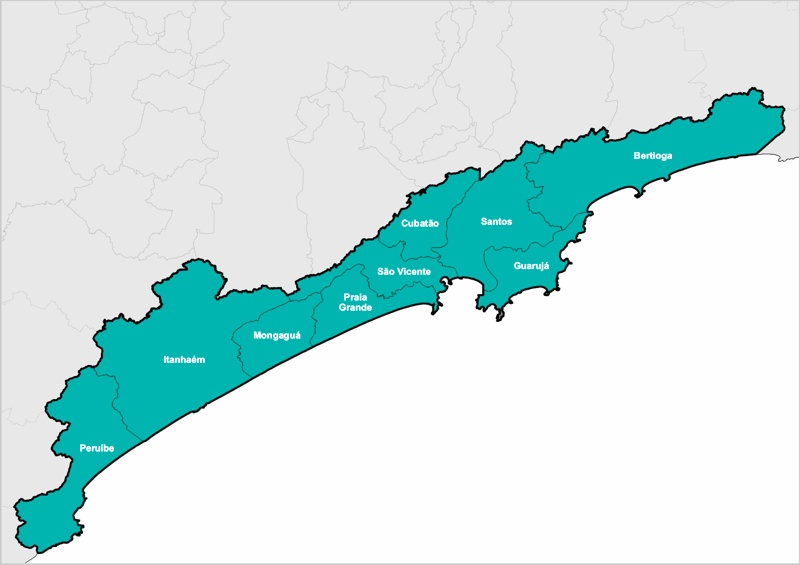
\includegraphics[width=20cm,height=20cm,keepaspectratio]{img/mapa_RMBS_emplasa.jpg}
			\label{mapa_rmbs}
			\legend{Fonte: \citeonline{emplasa2017a}}
		\end{figure}
	\end{landscape}
	 
	A figura \ref{tab_distancias} aponta e resume as principais informações de distância da cidade em estudo com as demais de sua região metropolitana:
	
	\begin{table}[!htb]
		\centering
		\caption{Distâncias rodoviárias (da Capital e municípios da \gls{rmbs}) em relação à Praia Grande}
		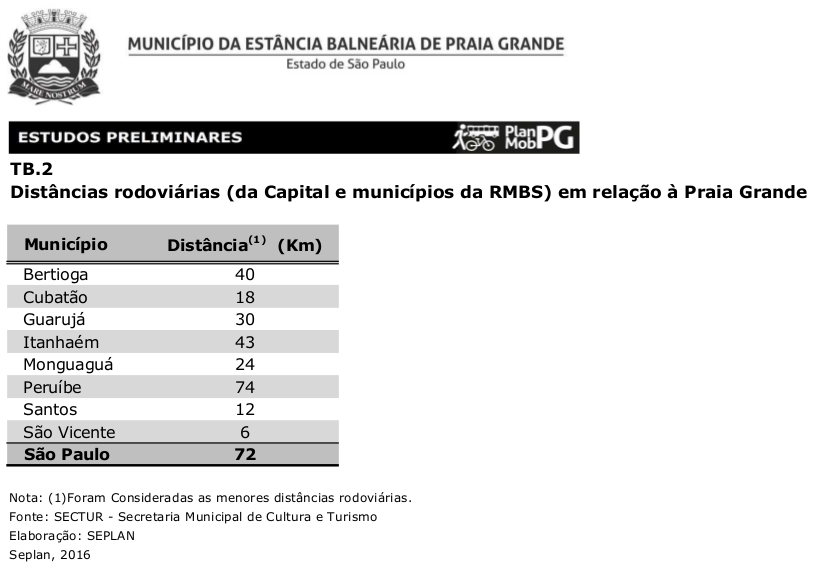
\includegraphics[width=1\textwidth]{img/TB_2_DISTANCIAS_RODOVIARIAS.png}
		\label{tab_distancias}
		\legend{Fonte: \citeonline{secplan2016a}}
	\end{table}
	% Parte do Anderson
		
	\subsection{Breve histórico do município}
	
	Conforme \citeonline[p.45]{imario2008a}, ``muito tempo antes da construção da Fortaleza do Itaipu, se deu a colonização irregular do Japuí e da área situada às margens do Mar Pequeno, a qual pertencia a São Vicente e onde hoje está localizada a cidade de Praia	Grande''. \citeonline[p.54]{imario2008a} também comenta que ``até as primeiras décadas do século XX, o distrito de Praia Grande, sobrevivia de uma agricultura de subsistência e da exploração dos seus recursos naturais, traços básicos da economia brasileira da época'', inclusive comercializando lenha com a \gls{efs} e o Porto de Santos.

	% Parte do Anderson
	A área que hoje é o município de Praia Grande foi um distrito, parte do município de São Vicente até a década de 1960. O município foi emancipado em 19 de janeiro de 1967, após várias lutas no decorrer das décadas de 1950 e 1960 que reivindicavam melhores condições de infraestrutura na região.
	
	Até hoje permanece a divisão do município em 2 distritos: Praia Grande e Solemar, que foram os distritos desmembrados de São Vicente para formar o município de Praia Grande.
	
	Com a construção da Ponte do Mar Pequeno, na década de 1980, o município se tornou a área de praia mais próxima da capital paulista, dessa forma atraindo muitos turistas, principalmente os turistas de um dia, de baixa renda. O comércio nessa época se adequa às necessidades desse perfil de turista. No entanto, o perfil tem mudado nos últimos anos.
	% Parte do Anderson
	
	\citeonline{Rolnik2000a} apontava em 2000 a predominância de um caráter periférico no município:
	
	\begin{citacao}
		Na Baixada Santista, Cubatão, Praia Grande, São Vicente e Mongaguá são municípios que funcionam como periferia de Santos. É importante ressaltar que, na região, incluindo as cidades-pólo, não se encontram municípios com mais de 60\% de domicílios em situação adequada (a cidade de Campinas é a única exceção). Trata-se de uma macrorregião, a mais dinâmica e rica do Estado de São Paulo,5 onde se operou uma “desconcentração concentrada” da indústria e de pólos de serviços, em um raio de 150 km da capital. Essa região delimita, do ponto de vista urbanístico, o raio de um padrão de expansão urbana baseado na grande indústria, no transporte sobre rodas e na expansão periférica da habitação de baixa renda, espraiando precariedade urbana e exclusão territorial em suas fronteiras.
		
		(\dots)
		
		Essas cidades ou são balneários/ estâncias com um perfil semelhante ao mencionado anteriormente (Caraguatatuba e Atibaia), ou cidades-dormitório da periferia metropolitana (Embu, Embu-Guaçu e Rio Grande da Serra).
		\cite[p.78]{Rolnik2000a}
	\end{citacao}
	
	\subsection{Aspectos demográficos atuais}
	
	Com uma população estimada em 310.024 habitantes para o ano de 2017 \cite{ibge2017a} ante o levantamento anterior do Censo 2010 do \gls{ibge}, que dava conta de 262.051 habitantes no município \cite{ibge2017a}, sendo que ``entre 2000 e 2010, a população de Praia Grande cresceu a uma taxa média anual de 3,07\%, enquanto no Brasil foi de 1,17\%, no mesmo período'' \cite{atlas2017a}.

	% Parte do Anderson
	Com população de 262.051 pessoas e densidade demográfica de 1.781,87 pessoas, segundo o Censo 2010 realizado pelo Instituto Brasileiro de Geografia e Estatística (IBGE), Praia Grande aponta para o ano de 2017, população equivalente a 310.024 pessoas e densidade de 2.016,87, números que, apesar de condicionaram avanço de 18\% nos números de contagem populacional, simbolizam o resultado de um “decrescente” processo de crescimento da população. De acordo com dados disponibilizados pela Fundação SEADE em sua seção pública de informações dos perfis municipais do estado de São Paulo, as Taxas de Crescimento Geométrico Anual (TGCA) do município vem apresentando sensíveis quedas desde o ano de 1991 até hoje, conforme tabela \ref{tab_tgca}.
	
	\begin{center}
		\begin{longtable}{|l|l|}
			\caption{Taxa Geométrica de Crescimento Anual da População (em \% a.a.).} \label{tab_tgca}\\
			\hline
			\textbf{Ano} & \textbf{Taxa} \\
			\hline
			\endfirsthead
			\multicolumn{2}{c}%
			{\tablename\ \thetable\ -- \textit{Continuado da página anterior}} \\
			\hline
			\textbf{Ano} & \textbf{Taxa} \\
			\hline
			\endhead
			\hline \multicolumn{2}{r}{\textit{Continua na próxima página}} \\
			\endfoot
			\hline
			\endlastfoot
			1991 & 5,86 \\
			2000 & 5,18 \\
			2010 & 3,09 \\
			2017 & 2,04 \\
		\end{longtable}
		\legend{Elaboração própria. Fonte: \citeonline{seade2017a}}
	\end{center}
	
	Ainda de acordo com os dados do Censo 2010, realizado pelo IBGE, o município de Praia Grande apresentava estrutura populacional determinada pela pirâmide etária da figura \ref{pira_etaria}, que revela um panorama no qual cerca de 45\% de toda a população residente do município está concentrada na faixa etária de 20 a 50 anos de idade. Deste montante, entre os homens, 46\% se enquadram neste padrão e, entre as mulheres, 45\%.
	
	\begin{figure}[!htb]
		\centering
		\caption{Pirâmide Etária}
		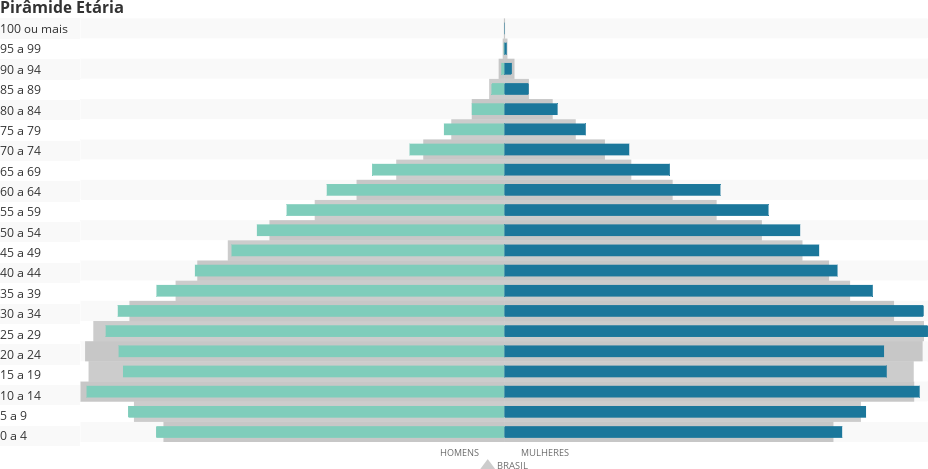
\includegraphics[width=1\textwidth]{img/ibge2017c_pira_etaria.png}
		\label{pira_etaria}
		\legend{Fonte: \citeonline{ibge2017c}}
	\end{figure}
	
	Já no que tange aspectos raciais, o município é estava caracterizado por uma distribuição predominantemente tomada por pessoas que autodeclararam-se de cor branca, conforme figura \ref{comp_racial}.

	\begin{figure}[!htb]
		\centering
		\caption{Praia Grande \textendash Distribuição Percentual da População Segundo Cor ou Raça -- 2010}
		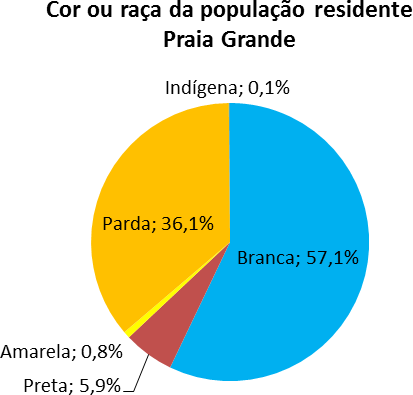
\includegraphics[width=0.5\textwidth]{img/polis_raca.png}
		\label{comp_racial}
		\legend{Fonte: \citeonline[p.17]{Polis2013a}}
	\end{figure}
	
	\subsection{Economia e trabalho}
	
	Com Produto Interno Bruto, a preços correntes, registrado em 2014, de R\$ 5.512.844.000,00 e PIB per capita de R\$ 18.770,64, a cidade é sobremaneira representada economicamente por intensas atividades comerciais e de serviços. Cerca de 60\% de toda a soma de riquezas municipal provém do terceiro setor da economia, onde, o valor adicionado do PIB chegou à marca de R\$ 3.403.806.000,00, isto é, aproximadamente, 5 vezes mais que o corresponde a produção industrial. Deste montante tão substancial na participação do terceiro setor no PIB da região, 26\%, isto é, R\$ 1.063.494,34 são provenientes de atividades ligadas a administração e serviços públicos, conforme tabela \ref{tab_pib}.

	Uma vez tão concentrada em um único setor, é natural que a atividade econômica central da região também induza a uma enorme concentração de empresas e empregos. Na cidade, onde 8331 empresas atuavam, em 2013, e 53.505 pessoas se configuraram em condição de ocupação e proporcionaram salário médio mensal de 2,5 salários mínimos, cerca de 60\% dos empregos formais também se concentrava no setor de serviços, como ilustrado na figura \ref{graf_empregados}.

	\begin{center}
		\begin{longtable}{|l|l|}
			\caption{Produto Interno Bruto de Praia Grande em 2013} \label{tab_pib}\\
			\hline
			\textbf{Setor} & \textbf{Valor} \\
			\hline
			\endfirsthead
			\multicolumn{2}{c}%
			{\tablename\ \thetable\ -- \textit{Continuado da página anterior}} \\
			\hline
			\textbf{Setor} & \textbf{Valor} \\
			\hline
			\endhead
			\hline \multicolumn{2}{r}{\textit{Continua na próxima página}} \\
			\endfoot
			\hline
			\endlastfoot
			Agropecuária 						& 2252,013		\\
			Indústria 	 						& 579910,463	\\
			Serviços 	 						& 2988331,997	\\
			Administração e Serviços Públicos	& 1063494,341	\\
			Impostos 							& 321175,59		\\
		\end{longtable}
		\legend{Elaboração própria. Fonte: \citeonline{ibge2017b}}
	\end{center}
	
	\begin{figure}[!htb]
		\centering
		\caption{Pessoas ocupadas por setor 2007--2013}
		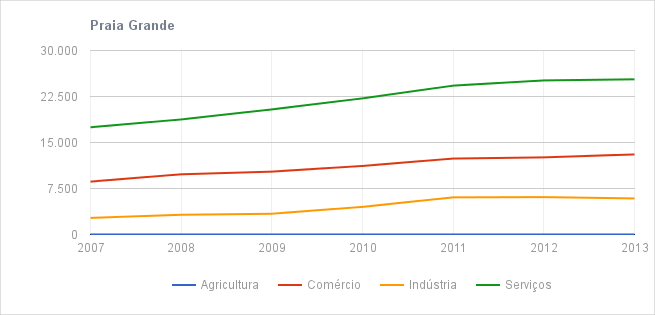
\includegraphics[width=1\textwidth]{img/graf_pessoas_empregadas.png}
		\label{graf_empregados}
		\legend{Fonte: \citeonline{ibge2017b}}
	\end{figure}
	% Parte do Anderson
	
	De acordo com \citeonline{Polis2013a} em seu diagnóstico da região de Praia Grande, em 2010, 128.806 pessoas totalizavam a população economicamente ativa (PEA) da cidade, isto é, 49\% de toda a população residente, de onde obtinha-se uma taxa de desocupação de 10,74\% e taxa de informalidade 42,73\% - índices superiores aos da própria Região Metropolitana da Baixada Santista, do Estado de São Paulo e do Brasil, conforme tabela \ref{tab_pea}.
	
	\begin{center}
		\begin{longtable}{l l l l}
			\caption{População Economicamente Ativa de Praia Grande em 2010} \label{tab_pea}\\
			\hline
			\textbf{Região} & \textbf{PEA} & \textbf{Taxa de desocupação} & \textbf{Taxa de informalidade} \\
			\hline
			\endfirsthead
			\multicolumn{4}{c}%
			{\tablename\ \thetable\ -- \textit{Continuado da página anterior}} \\
			\hline
			\textbf{Região} & \textbf{PEA} & \textbf{Taxa de desocupação} & \textbf{Taxa de informalidade} \\
			\hline
			\endhead
			\hline \multicolumn{4}{r}{\textit{Continua na próxima página}} \\
			\endfoot
			\hline
			\endlastfoot
			Praia Grande & 128.806 & 10,74 & 42,73 \\
			RMBS & 827 & 9,8 & 37 \\
			Estado de SP & 21.639.776 & 8,1 & 33 \\
			Brasil & 93.504.659 & 7,6 & 41 \\
		\end{longtable}
		\legend{Elaboração própria. Fonte: \citeonline[p.88]{Polis2013a}}
	\end{center}
	
	\subsection{Indicadores sociais}
	
	Praia Grande apresentava em 2016 uma área da unidade territorial de 149,253 km$^2$ \cite{ibge2017a}. No que tange ao \gls{idhm}, o município está situado entre aqueles que apresentam Alto Desenvolvimento:
	
	\begin{citacao}
		O Índice de Desenvolvimento Humano (IDHM) - Praia Grande é 0,754, em 2010, o que situa esse município na faixa de Desenvolvimento Humano Alto (IDHM entre 0,700 e 0,799). A dimensão que mais contribui para o IDHM do município é Longevidade, com índice de 0,834, seguida de Renda, com índice de 0,744, e de Educação, com índice de 0,692.
		\cite{atlas2017a}
	\end{citacao}
	
	\begin{figure}[!htb]
		\centering
		\caption{Evolução do IDHM -- Praia Grande - SP}
		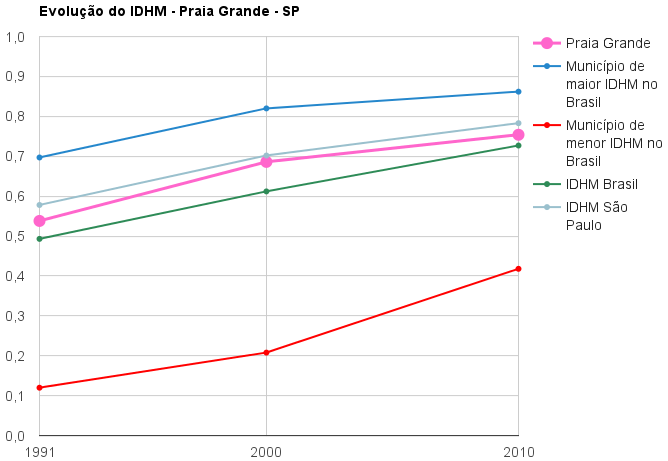
\includegraphics[width=0.8\textwidth]{img/atlas2017a_01.png}
		\legend{Fonte: \citeonline{atlas2017a}}
	\end{figure}
	
	No que diz respeito à renda:
	
	\begin{citacao}
		A renda per capita média de Praia Grande cresceu 54,85\% nas últimas duas décadas, passando de R\$ 530,16, em 1991, para R\$ 759,05, em 2000, e para R\$ 820,97, em 2010. Isso equivale a uma taxa média anual de crescimento nesse período de 2,33\%. A taxa média anual de crescimento foi de 4,07\%, entre 1991 e 2000, e 0,79\%, entre 2000 e 2010. A proporção de pessoas pobres, ou seja, com renda domiciliar per capita inferior a R\$ 140,00 (a preços de agosto de 2010), passou de 13,22\%, em 
		, para 10,71\%, em 2000, e para 5,95\%, em 2010. A evolução da desigualdade de renda nesses dois períodos pode ser descrita através do Índice de Gini, que passou de 0,49, em 1991, para 0,55, em 2000, e para 0,49, em 2010.
		\cite{atlas2017a}
	\end{citacao}
	
	% = = = = = =
		
	\section{Ordenamento territorial} \label{ord_territorial}
	
	\subsection{Macrozoneamento}
	
	O macrozoneamento estabelecido conforme as Diretrizes de Ordenamento Territorial dispostas no Plano Diretor vigente em 2017 muito dizem sobre a configuração espacial do município, bem como sobre tendências territoriais. Desse modo, o município é segmentado em sete grandes áreas \cite[Art. 101]{pmpg2016a}: 
	
	\begin{enumerate}[label=\alph*)]
		\item Parque Estadual da Serra do Mar/Morro do Estaleiro e Parque Estadual do Xixová-Japuí, áreas de preservação com Planos de Manejo já desenvolvidos e a serem implementados pelo Instituto Florestal; 
		\item Parque do Piaçabuçu, que configura área de preservação e lazer, carecendo ainda de Plano de Manejo, a ser desenvolvido e implementado pelo município através da Unidade da administração direta competente;
		\item Área de Transição caracteriza a área de proteção do Parque Estadual da Serra do Mar perante à pressão antrópica e de preservação dos remanescentes da restinga. Área destinada a atividades de apoio urbano e turismo ecológico, além de baixa intensidade de ocupação;
		\item Área Residencial Especial compreende a área de restinga sujeita a pressão antrópica, demanda padrão de ocupação de baixa densidade e conservação de compartimentos significantes da vegetação natural;
		\item Área Predominantemente Residencial representa a área densamente ocupada e que comporta atividades comerciais e serviços associados ao uso residencial ;
		\item Área Comercial de Âmbito Regional tem localização privilegiada com relação ao assentamento urbano consolidado e sistema viário que possibilita conexão intermunicipal e regional do município;
		\item Área de Usos Diversificados de Porte Regional compreende faixa ainda não parcelada, mas de privilegiada localização com relação aos modais rodoviários e ferroviários, possui incompatibilidade com o uso residencial.
	\end{enumerate}
	
	%	Essas áreas seguem padrão determinado pela mais recente Lei de Uso e Ocupação do Solo (Lei n\textordmasculine 615/2011), onde o zoneamento do município se divide em 7 grandes grupos, que podem conter subdivisões e apresentam um conjunto de características:
	
	De acordo com a mais recente Lei de Uso e Ocupação do Solo (Lei n$^{o}$ 615/2011), que pode ser visto na figura \ref{mapa_zoneamento}, as zonas no Município se dividem em 7 grandes grupos, que podem conter subdivisões e apresentam um conjunto de características \cite[Cap. II, Art. 9\textordmasculine]{pmpg2011a}:
	
	\begin{itemize}
		\item Zona Exclusivamente Residencial (ZR);
		\item Zonas Predominantemente Residenciais (ZPR-1, ZPR-2 e ZPR-3);
		\item Zonas Comerciais (ZC-1, ZC-2, ZC-3 e corredores comerciais);
		\item Zona Mista (ZM);
		\item Zona de Usos Diversificados (ZUD-1 e ZUD-2);
		\item Zona de Transição (ZT);
		\item Zona Especial de Interesse Ecológico (ZEIE-1, ZEIE-2 e ZEIE-3).
	\end{itemize}
	
	\begin{landscape}
		\begin{figure}[h]
			\centering
			\caption{Zoneamento em Praia Grande de acordo a LPUOS de 2011}
			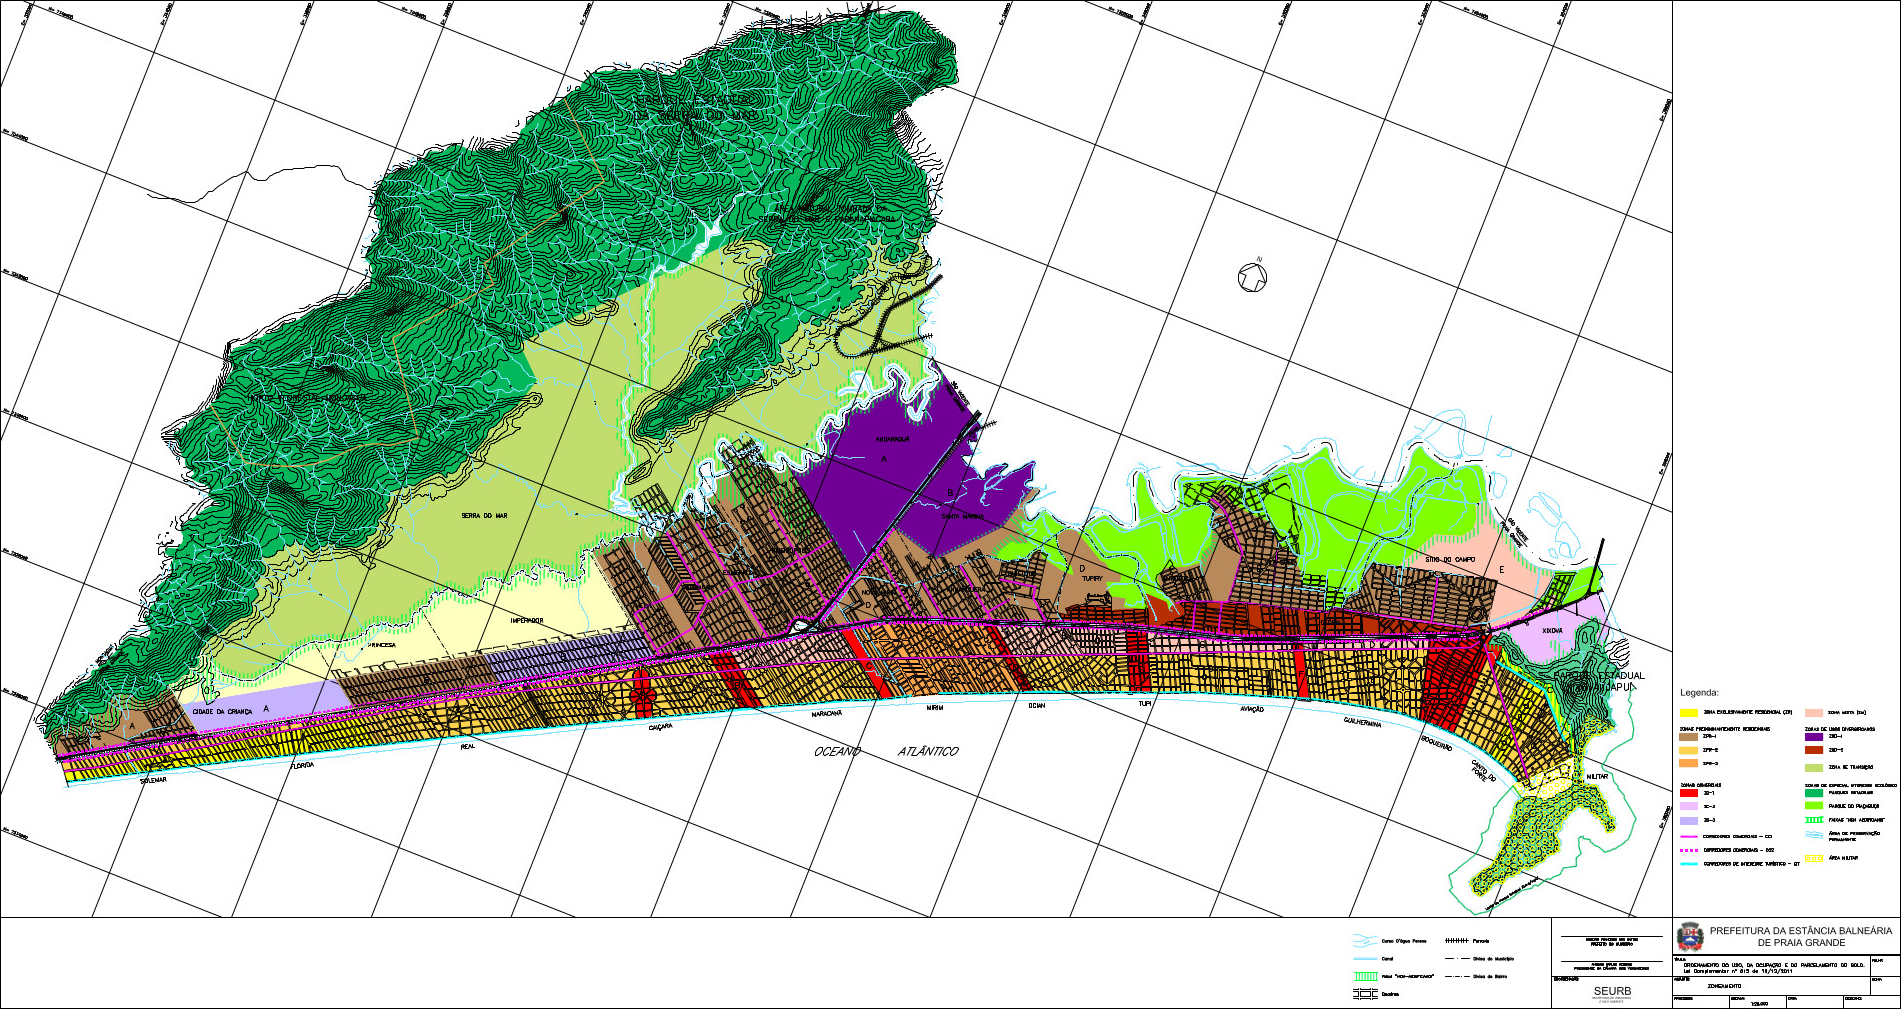
\includegraphics[width=25cm,height=25cm,keepaspectratio]{img/3788_Carta_Oficial_Zoneamento.jpg}
			\label{mapa_zoneamento}
			\legend{Fonte: \cite{pmpg2011a}}
		\end{figure}
	\end{landscape}
	
	A lei disciplina o parcelamento do solo de acordo com a Tabela \ref{quadro_parcelamento}.
	
	\begin{table}[H]
		\centering
		\caption{Índices Normativos Para o Parcelamento}
		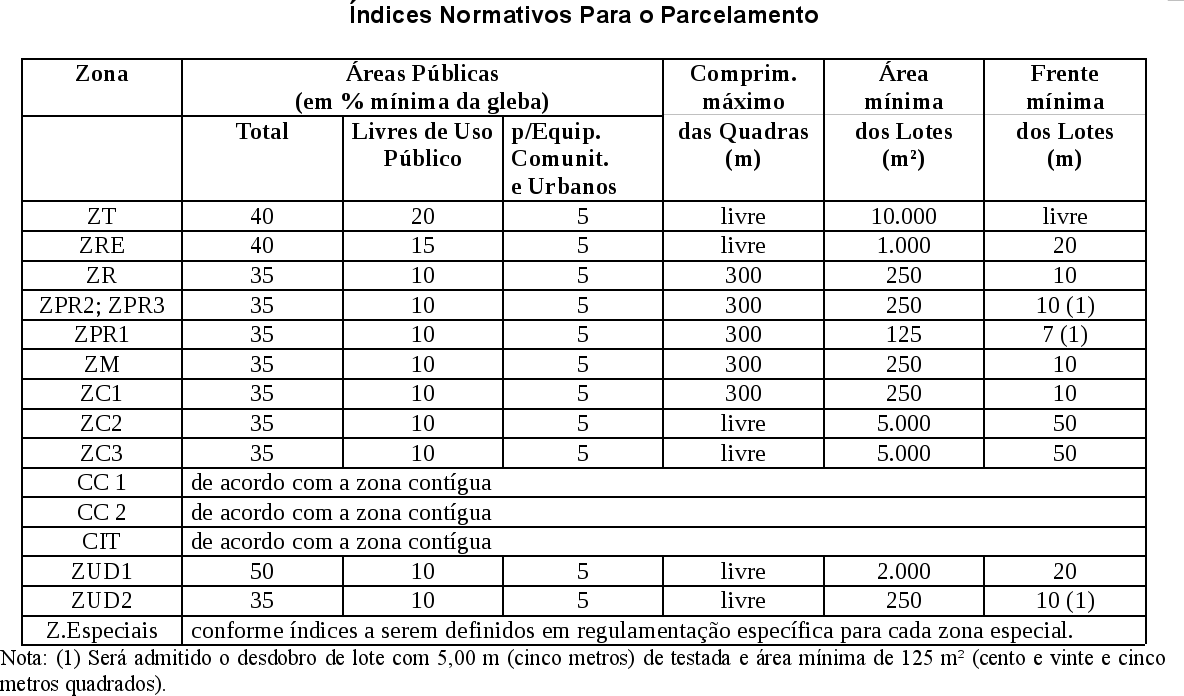
\includegraphics[width=1\textwidth]{img/id_parcelamento.png}
		\label{quadro_parcelamento}
		\legend{Fonte: \citeonline[Art. 55]{pmpg2011a}}
	\end{table}
	
	Em visita de campo realizada no dia 25/10/2017, foram observados grandes lotes não edificados situados junto à orla, o que levou ao questionamento acerca da aplicação da PEUC, instrumento que prevê o Parcelamento, Edificação e Utilização Compulsórios a fim de garantir o cumprimento da função social da propriedade urbana. 
	
	Os artigos que disciplinam a \gls{peuc} no Plano Diretor disciplinam que as áreas passíveis de aplicação do instrumento devem ser delimitadas pelo \gls{pde}, dotadas ou dotáveis de infra-estrutura, destinadas a projetos habitacionais de interesse social ou projetos de interesse econômico e também áreas que não possuam pendências jurídicas. O coeficiente de aproveitamento mínimo é alto, o que também configura impasse à aplicação do instrumento.
	
	\subsection{Complexo Andaraguá}
	
	O Complexo Andaraguá é um empreendimento empresarial e aeroportuário a ser implementado em área delimitada pelo Plano Diretor como área de uso diversificado de porte regional. Embora o terreno tenha cerca de 12km$^{2}$, 70\% deve ser preservado, o que coloca em xeque a coerência do zoneamento. A área aproveitada é ainda bastante extensa, conta com 5km$^{2}$, aproximadamente três vezes maior que o aeroporto de Congonhas.
	
	O projeto prevê, além de aeroporto e estacionamento para caminhões, a construção de galpões, a fim de alugá-los a mais de duzentas empresas nos setores de exportação, indústria de tecnologia, química e bioquímica, farmacêuticas e hospitalares, de automóveis, autopeças, componentes para aviação, máquinas industriais, componentes eletrônicos, entre outros \cite{Incipar2017a}.
	
	Tratando-se de um empreendimento de grande porte, é passível de questionamento se os parâmetros de incomodidade estabelecidos pela \gls{luops} foram subdimensionados no estudo de impacto ambiental, visto que o bairro Andaraguá se situa entre área de transição e áreas predominantemente residenciais, classificadas em grande parte como \gls{zeis} devido a concentração de assentamentos precários. 

	% = = = = = =
	
	\section{Ambiente urbano}
	% Foram mescladas as partes do Henrique e da Jade
		
	A partir da análise do processo de ocupação do município da Praia Grande, decorrente de suas características e potencialidades naturais, sociais e econômicas, é possível compor um retrato geral.
	
	\subsection{Características fisiográficas}
	% Parte da Jade
	
	O município de Praia Grande possui uma área total de 149,25 km$^2$, mas parte significativa do seu território se insere em áreas de conservação e permanece não ocupada, influenciando na baixa densidade populacional total do município. A área efetivamente urbanizada corresponde a 26\% do território e resulta numa densidade populacional de 66hab/ha \cite{ls2012a}. Grande parte da população do município está concentrada no distrito de Praia Grande, que envolve a região central e divisa com São Vicente. Por sua vez, a maior parte da área urbanizada do município possui densidade populacional de 250hab/ha \cite{ls2012a}.
	
	O município é dividido em dois distritos, o distrito de Praia Grande e o distrito de Solemar (Figura \ref{mapa_solemar_pg}).
	
	\begin{figure}[!htb]
		\centering
		\caption{Distrito de Praia Grande e Distrito de Solemar}
		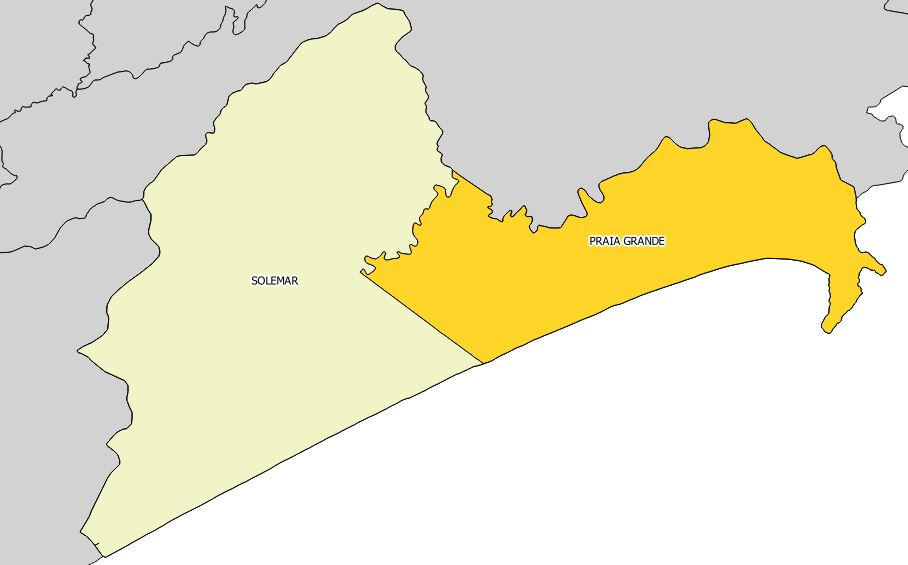
\includegraphics[width=1\textwidth]{img/Distritos_Praia_Grande.jpg}
		\label{mapa_solemar_pg}
		\legend{Elaboração própria}
	\end{figure}
	
	Conforme veremos na seção \ref{ord_territorial}, o zoneamento reforça que as áreas mais dinâmicas e com maior presença de infraestrutura estão concentradas na região de orla da praia e no distrito de Praia Grande, assim como a maior presença de zonas e corredores comerciais\footnote{Marcados nas tonalidades vermelha e rosa, conforme poderá ser conferido adiante na Figura \ref{mapa_zoneamento}}. Da mesma forma, o zoneamento já chama atenção para a presença de áreas com pouca provisão de infraestrutura e com predominância de uso residencial, as chamadas ZPR-1, que estão concentradas principalmente ao longo da rodovia Padre Manoel da Nóbrega (SP-55).
			
	\subsection{Identificação de usos}
	
	Praia Grande é um destino turístico consolidado que gera intenso deslocamento e grandes fluxos de população flutuante, o que atribuiu ao município o título de “Estância Balneária”\footnote{Conforme sublinha \citeonline[p.22]{imario2008a}, ``Foram 	inúmeras as obras de transformação da paisagem e melhoramentos urbanos	promovidos pelas sucessivas gestões municipais em sua orla marítima e adjacências. Estas mudanças fizeram de Praia Grande, uma estância balneária cada vez mais atrativa para a atividade turística, para a indústria da construção	civil, e o seu uso, para tais fins, pressupõe mudanças na paisagem do lugar}, segundo Lei Estadual aprovada em outubro de 1979 \cite{gesp1979a}, doze anos após sua emancipação do município de São Vicente.
	
	De modo geral, o uso do solo do município é relativo ao seu caráter turístico. Salvo o uso ambiental devido ao Parque Estadual da Serra do Mar, que ocupa expressiva parcela do território, Praia Grande é predominantemente residencial, com grande quantidade de domicílios de uso ocasional. A região da orla e o centro concentram loteamentos de uso misto e comercial. Durante a visita guiada, a Secretaria de Planejamento revelou que aproximadamente 80 mil domicílios são de uso permanente, enquanto cerca de 110 mil são de uso ocasional, a maioria com o \gls{iptu} adimplente.
	
	\subsubsection{Centralidades}
	% Fonte citada no primeiro parágrafo não pôde ser encontrada. Alterei por outra
	A principal centralidade de Praia Grande envolve os bairros Boqueirão, Canto do Forte e Guilhermina, caracterizando-se por forte verticalização, fenômeno ainda mais concentrado nas quadras próximas da orla, tendência que já se apresentava intensa na caracterização realizada por \cite{agem2015a}. No entorno desta, bairros como Militar, Xixová e Sítio do Campo fazem limite com o município de São Vicente.
	
	Essa centralidade concentra grande parte das atividades econômicas do município, possui grandes supermercados, imobiliárias, correios, lojas, consultórios, revendedoras de automóveis etc. Litoral Plaza Shopping, único \textit{shopping center} do município, também está localizado nessa região, em área delimitada pelo Plano Diretor como Área Comercial de Âmbito Regional devido a localização privilegiada em relação aos sistemas viários municipal e intermunicipal, além de ser destinada a equipamentos, comércio e serviços de âmbito regional.
	
	A infraestrutura urbana é também concentrada nesses três bairros. Aspectos como saneamento básico, iluminação pública, pavimentação, guia, equipamentos de saúde, educação e lazer podem inclusive ser considerados satisfatórios. No entanto, a grande quantidade de população flutuante em alta temporada acarretam em problemas de abastecimento \cite{Lima2008a}, contudo, durante a visita monitorada, as funcionárias da prefeitura explicaram que obras realizadas pela \gls{sabesp} nos últimos 5 anos elevaram a resiliência do sistema de abastamento, sendo um exemplo recente a construção de um novo reservatório:
	
	\begin{citacao}
		``O governador do Estado de São Paulo, Geraldo Alckmin, inaugurou hoje (31), às 13h30, um novo reservatório, no município de Praia Grande. Com capacidade de 25 milhões de litros, a caixa-d'água regional beneficiará os habitantes de Praia Grande e da área continental de São Vicente, além dos turistas que todos os anos quadruplicam a população durante a temporada de verão. São mais de 1 milhão de pessoas beneficiadas.
		
		Foram investidos R\$ 17,8 milhões para a construção do reservatório. Feito em concreto armado, possui quase nove metros de altura, 92 metros de comprimento, 63,4 metros de largura no maior lado e 29,5 no menor lado. A caixa-d'água regional é alimentada por duas entradas independentes e recebe, por meio de adutoras, a água tratada nos sistemas produtores Mambu/Branco e Melvi, que chega pronta para distribuição e com qualidade para consumo.'' \cite{Sabesp2017b}
	\end{citacao}
	
	Adicionalmente, o bairro Mirim, concentra o chamado ``complexo administrativo'', que abriga o paço e a prefeitura, além de órgãos das justiças Estadual e Federal \cite{pmpg2014b}. Embora comparativamente seja ainda esvaziado, o Bairro Mirim tende ao aumento do comércio, setor de serviços e diversificação de atividades para suprir as demandas dos empreendimentos lá instalados.
	
	\subsection{Interesse turístico e cultural}
	
	Praia Grande segue um padrão muito singular de turismo de veraneio, cujo principal atributo é extensa praia urbana que possui boas conexões rodoviárias com a capital do Estado. Seus projetos de desenvolvimento são, portanto, voltados à população flutuante que se desloca às suas residências de uso ocasional no município, de forma a dificultar a elevação de demanda turística na baixa estação e causando grande desequilíbrio. 
	
	O diagnóstico realizado pela AGEM a fim de viabilizar o Plano Diretor de Turismo da Baixada Santista de 2002 apresentou uma avaliação dos tipos de meios de hospedagem de turismo e as características predominantes em cada município. À época, Praia Grande contava com poucos leitos divididos em hotéis, pensões, flats e pousadas, mas grande quantidade de colônias de férias \cite[p.109]{agem2002a}.
	
	\noindent
	\begin{minipage}[b]{.53\textwidth}
		\captionof{figure}{Total de Leitos Percentual}
		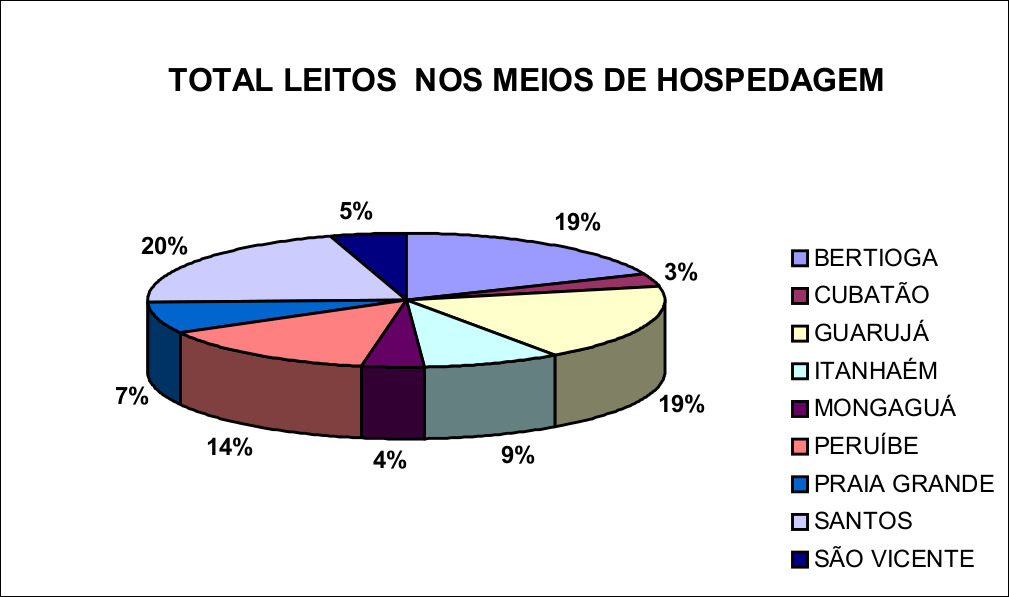
\includegraphics[width=\linewidth]{img/pdtur01.png}
		\legend{Fonte: \citeonline[p.107]{agem2002a}}
	\end{minipage}%
	\hfill
	\begin{minipage}[b]{.4\linewidth}
		\captionof{table}{Colônias de Férias da Região}
		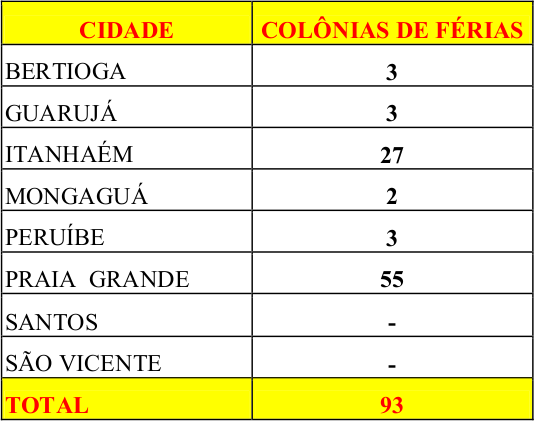
\includegraphics[width=\textwidth]{img/pdtur02.png}
		\legend{Fonte: \citeonline[p.108]{agem2002a}}
	\end{minipage}
	
	Foi feita ainda uma avaliação qualitativa dos atrativos culturais e naturais dos municípios, considerando os critérios de: 
	
	\begin{itemize}
		\item Acesso
		\item Sinalização externa
		\item Sinalização interna
		\item Segurança
		\item Estado de conservação externo
		\item Limpeza e manutenção
		\item Atendimento
		\item Monitoramento 
		\item Sistema atual	
	\end{itemize}
		
	Os atrativos listados foram a Fortaleza de Itaipu, o Portinho, as feiras de artesanato, a Capela Nossa Senhora da Guia, o Monumento Netuno e a Estátua de Iemanjá. Salvo a Fortaleza, classificada como ``ótimo'' em todos os critérios, o balanço dos atrativos foi ``não satisfatório''\footnote{O diagnóstico também menciona o Portal da Cidade, contudo, conforme constatado na visita monitorada, este fora demolido e a entrada da cidade conta apenas com um monumento mais discreto no canteiro central do viário, o qual conta com as iniciais PG} \cite[p.66-68]{agem2002a}.
	
	\begin{figure}[!htb]
		\centering
		\caption{Portinho}
		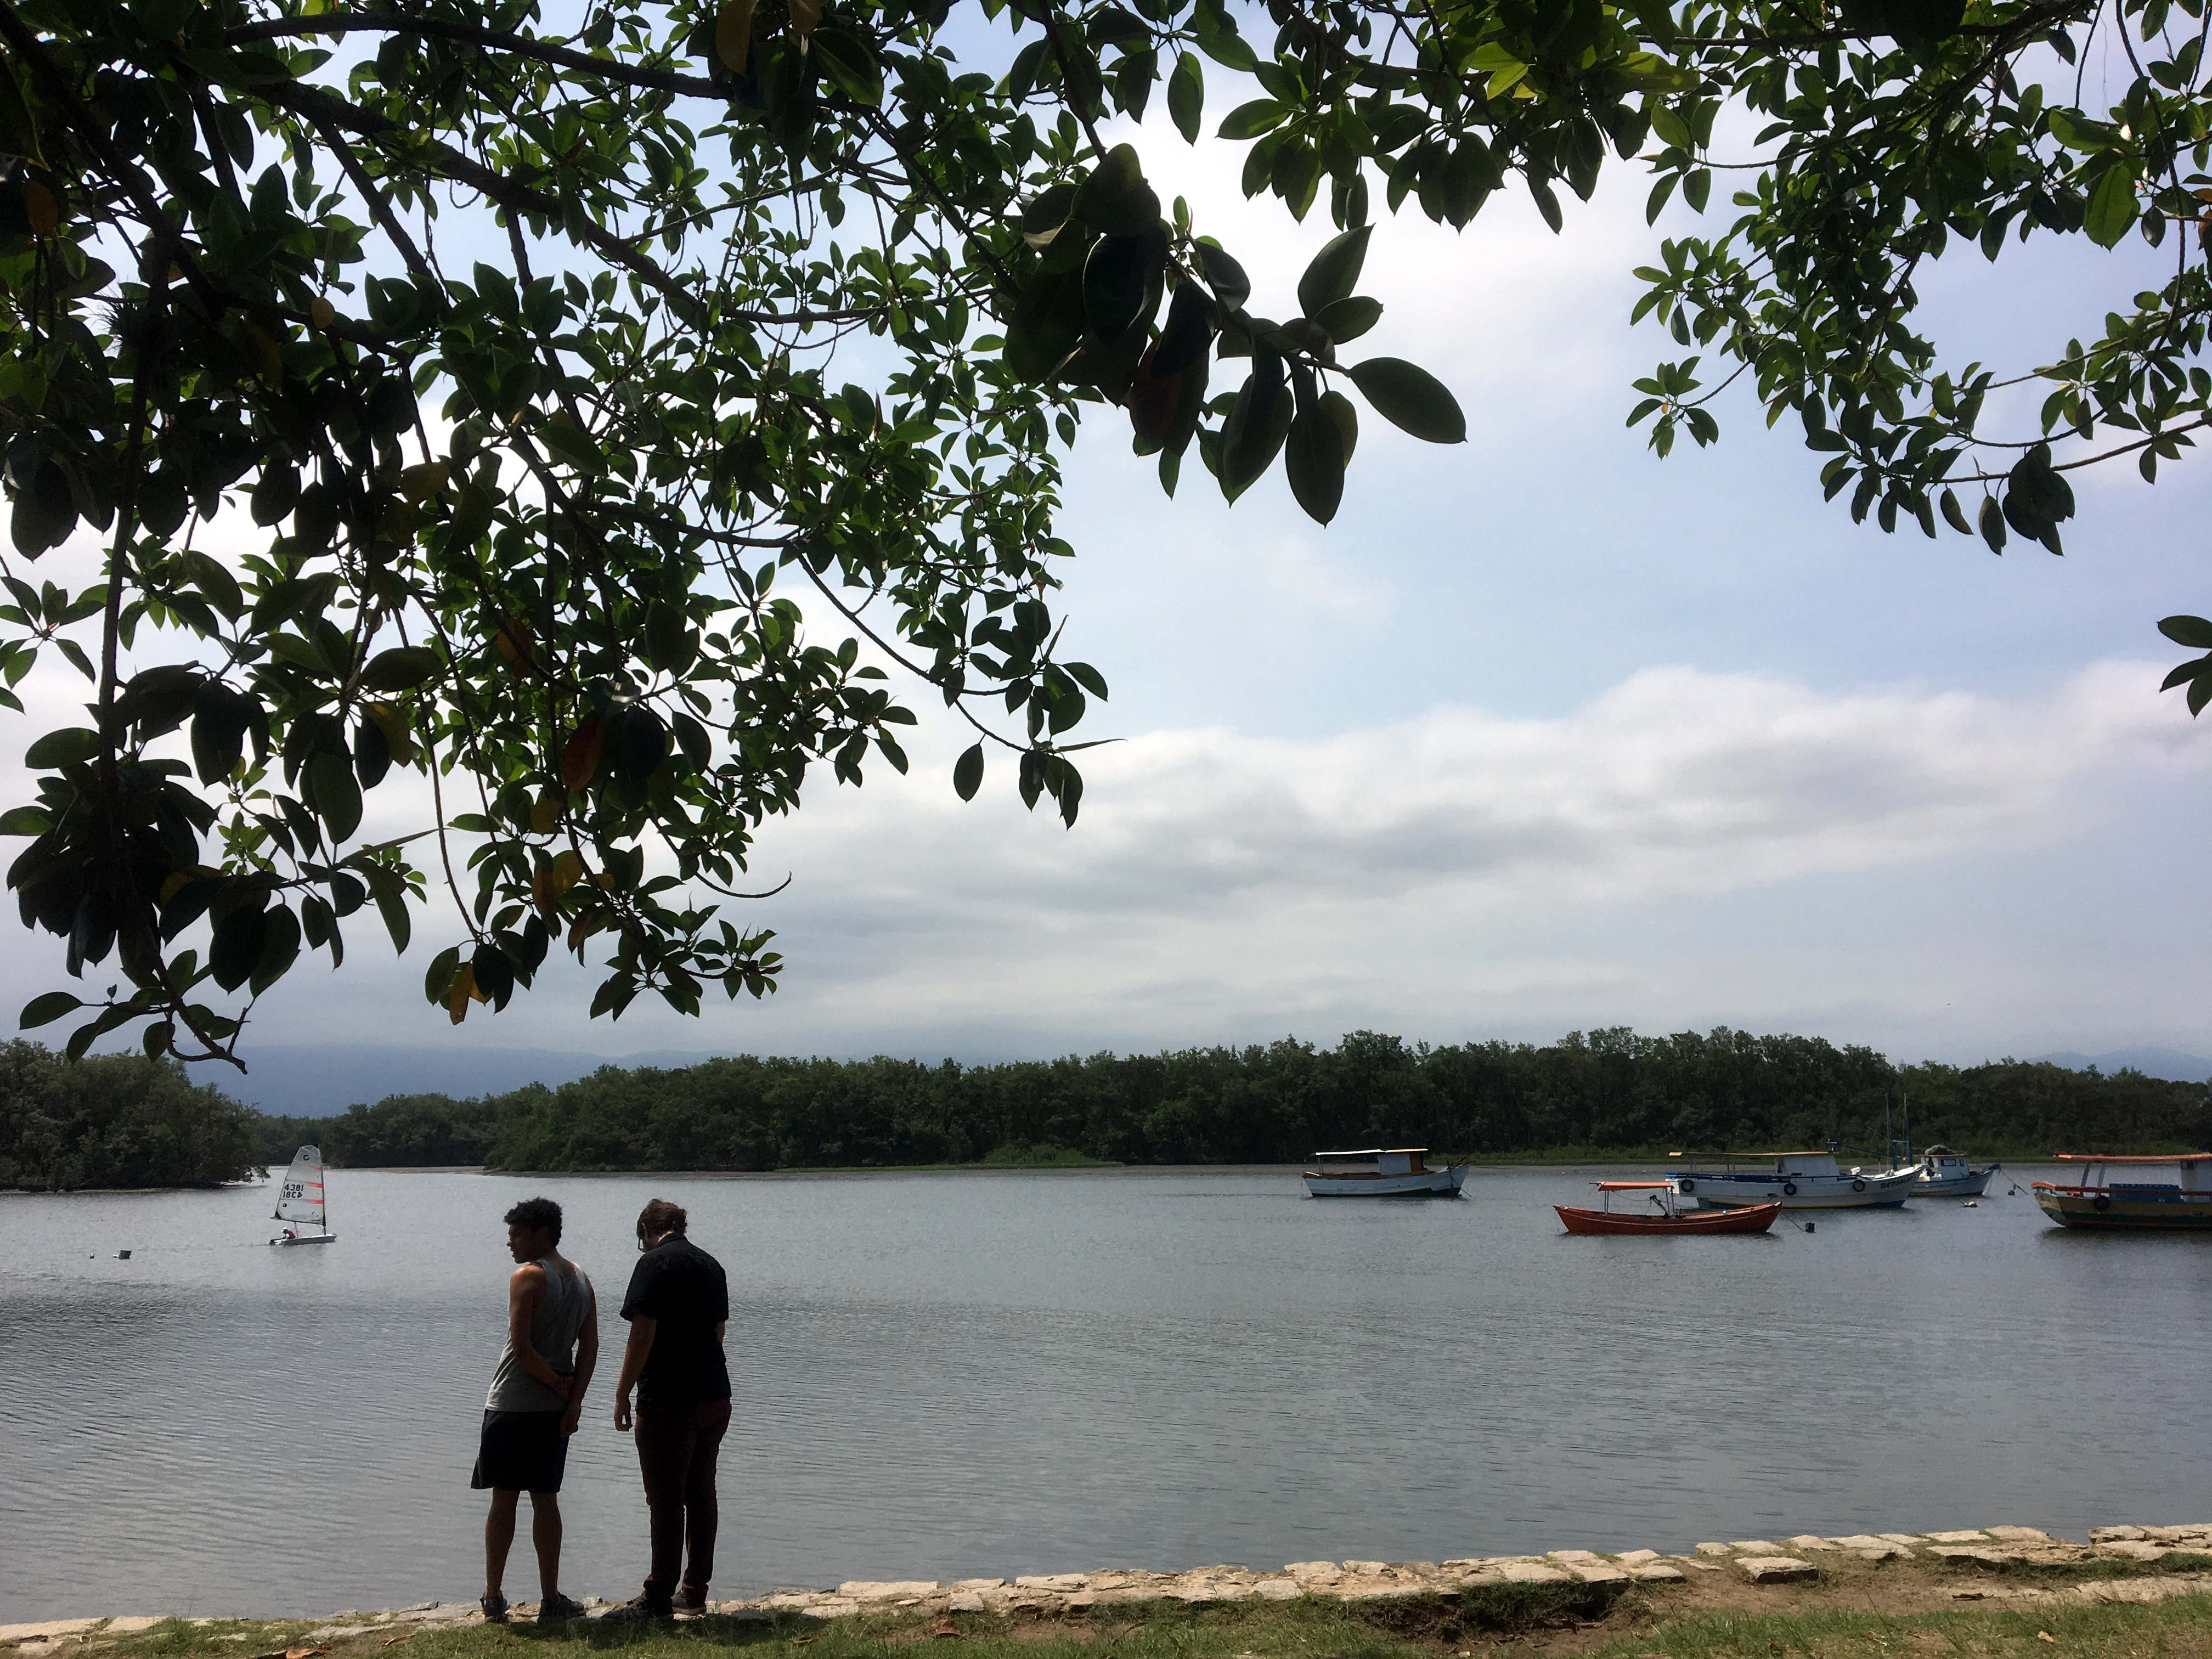
\includegraphics[width=0.6\textwidth]{img/IMG_2004.JPG}
		\legend{Elaboração própria}
	\end{figure}
	
	Os tipos de hospedagem descritos relacionam-se às potencialidades identificadas pelo relatório nos segmentos de turismo esportivo, náutico, ecológico, social e de terceira idade. 
	
	Atualmente, a cidade conta também com o Palácio das Artes, complexo cultural inaugurado em 2008, que oferece à cidade teatro, museu e galeria de arte e salão de eventos com cerca de mil metros quadrados. O salão abriga também atividades comerciais, tais como a Feira de Imóveis da Praia Grande, que reúne construtoras e incorporadoras a fim de vender mais de mil unidades, prontas, em construção ou na planta \cite{atribuna2017a}.
	
	No entanto, percebe-se manutenção na lógica do turismo de veraneio e pouca intenção de exploração de outras possibilidades turísticas. O Plano Diretor de Turismo Municipal está em fase de elaboração, o que abre espaço para que as questões apontadas sejam objeto de políticas públicas.
	
	\subsection{Padrões espaciais}
	
	Os municípios do litoral paulista passam, desde 2000, por um crescente processo de fixação de moradores e Praia Grande segue essa tendência. A distribuição no território dos domicílios de uso ocasionais e dos domicílios ocupados segue um manifesto padrão espacial e revela desigualdades. Os domicílios de uso ocasional concentram-se nos setores censitários ao longo da faixa litorânea, enquanto os domicílios ocupados pela população residente situam-se no interior da Rodovia Padre Manoel da Nóbrega.
	
	\begin{figure}[tb]
		\centering
		\caption{Distribuição percentual por classes de rendimento mensal de pessoas por domicílios (2010)}
		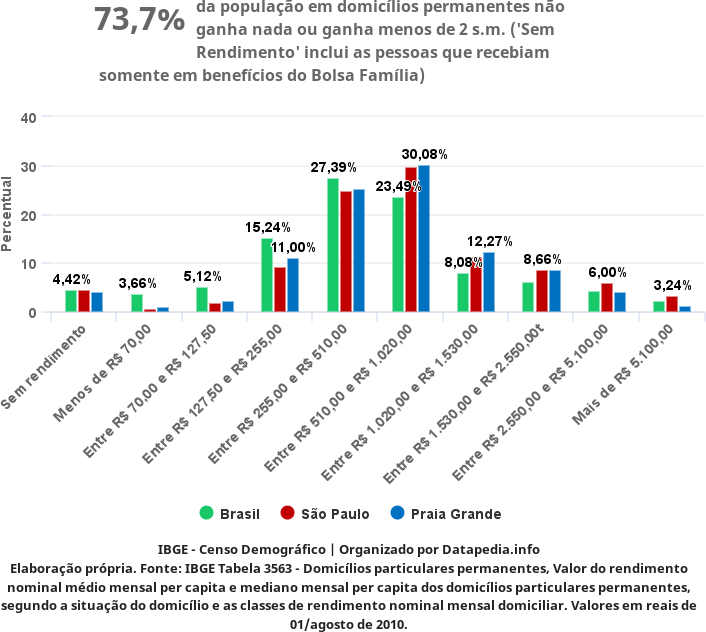
\includegraphics[width=0.7\textwidth]{img/datapedia.png}
		\label{mapa_datapedia}
		\legend{Elaboração própria. Fonte: \citeonline{Datapedia2017a}}
	\end{figure}
	
	Com exceção de Santos e Caraguatatuba, a população parda e preta dos municípios da RMBS apresentam taxas superiores às do Estado, e o município de Praia Grande acompanha essa dinâmica, somando 42\% de pretos e pardos. Uma análise preliminar do Mapa Racial do Brasil (vide recorte pertinente ao município, Figura \ref{mapa_racial_pata}) elaborado pela Post advertising technology agency (Pata) possibilita a identificação de padrões na distribuição étnico-racial da população praia-grandense. É nítida a concentração da população caracterizada como branca nos bairros mais próximos às faixas litorâneas, em contraste à heterogeneidade na face norte da Via Expressa Sul, principal rodovia urbana do município.

	Indicadores de renda ratificam, como esperado, a questão da segregação espacial.  Visando a visualização espacial da desigualdade, o critério utilizado pelo relatório realizado pelo Instituto Pólis foi o rendimento médio dos responsáveis pelos domicílios segundo os setores censitários. Desse modo, o indicador apontou que 62\% dos responsáveis por domicílios de Praia Grande possuem renda até 3 salários mínimos, dispersos pelo município mas com maior concentração também no eixo norte da rodovia, como pode ser visto na Figura \ref{mapa_3sm}.
	
	\begin{landscape}
		\begin{figure}[h]
			\centering
			\caption{Distribuição dos Percentuais dos Domicílios Particulares Permanentes Ocupados Segundo Setores Censitários - 2010}
			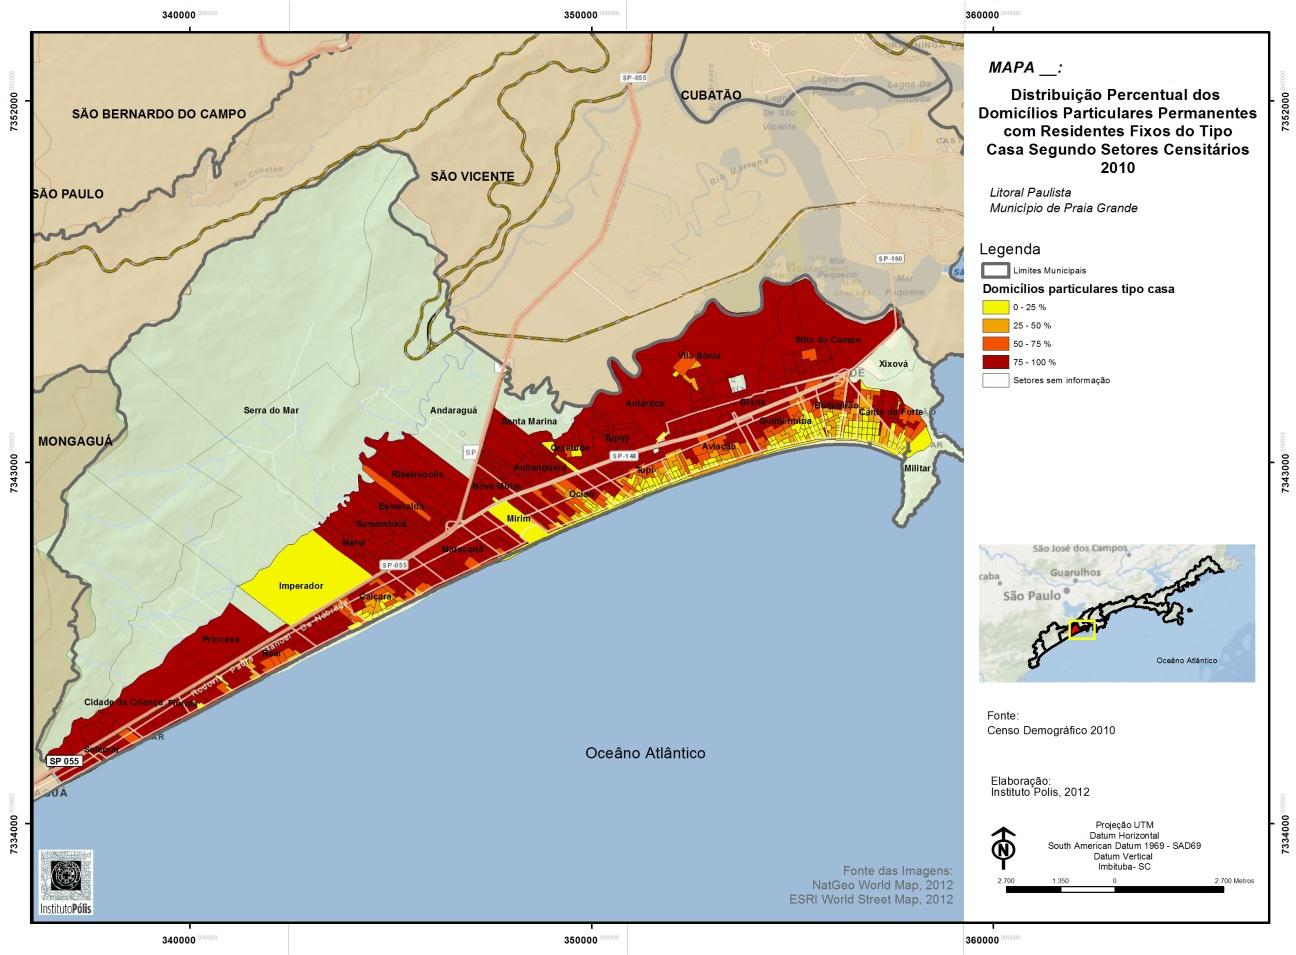
\includegraphics[width=20cm,height=20cm,keepaspectratio]{img/polis_fixos.png}
			\label{mapa_fixos}
			\legend{Fonte: \citeonline[p.32]{Polis2013a}}
		\end{figure}
	\end{landscape}

	\begin{landscape}
		\begin{figure}[h]
			\centering
			\caption{Mapa Racial do Brasil. Recorte: Praia Grande}
			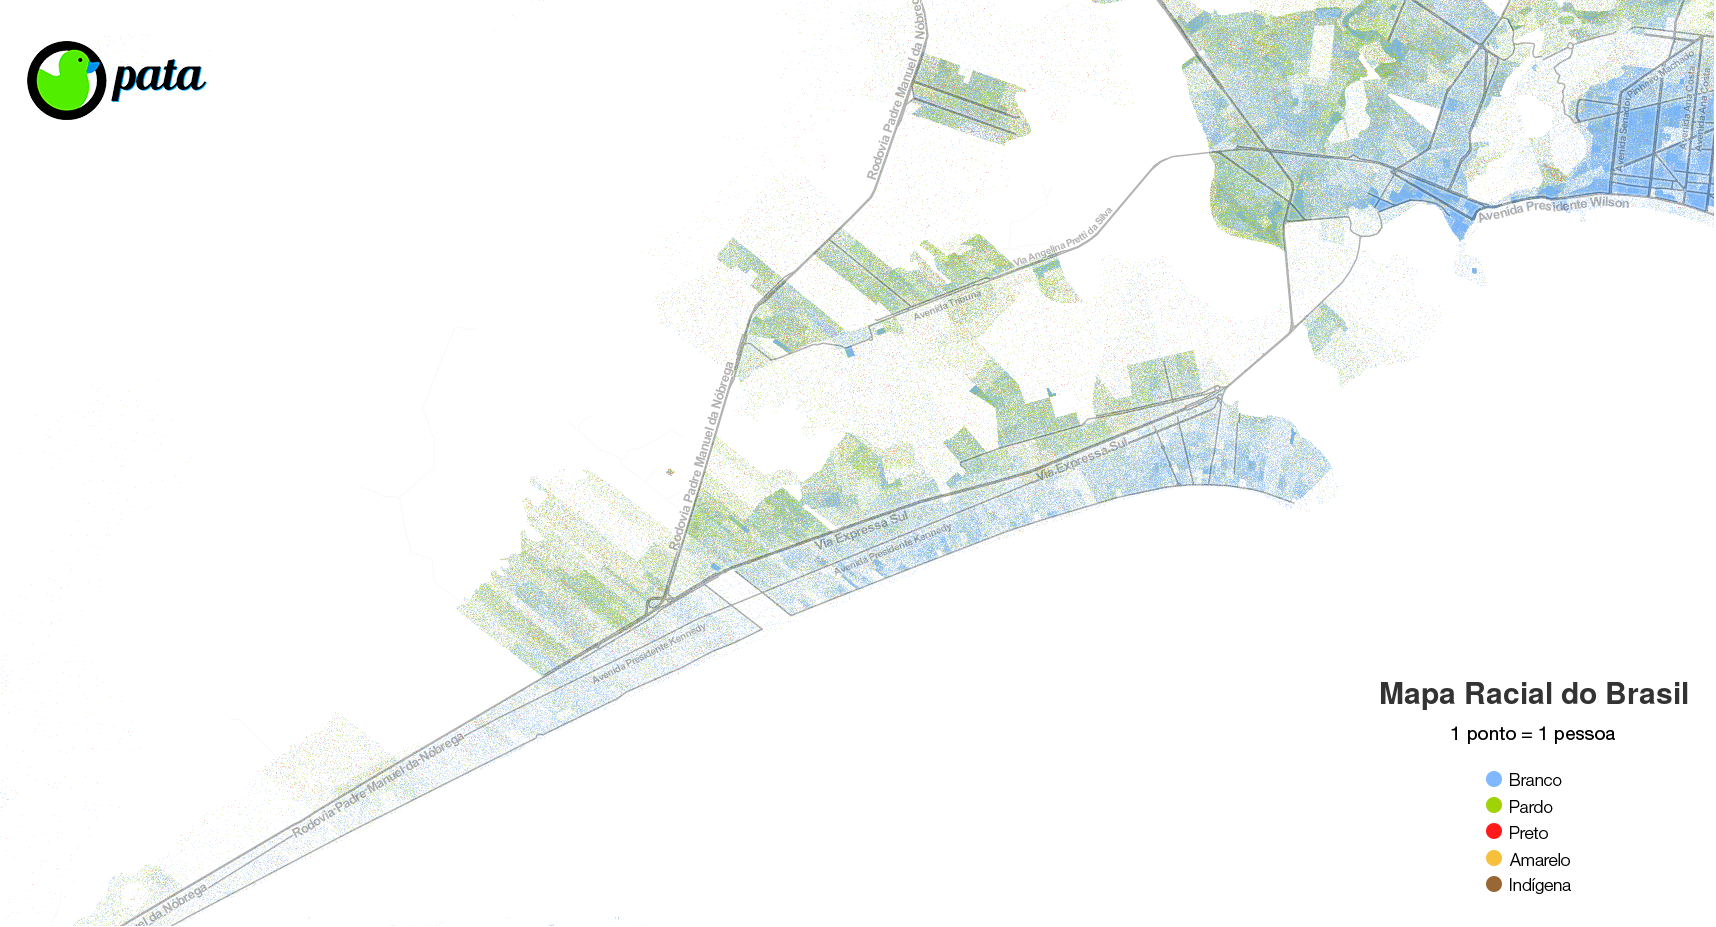
\includegraphics[width=25cm,height=24cm,keepaspectratio]{img/mapa_racial.png}
			\label{mapa_racial_pata}
			\legend{Elaboração própria. Fonte: \citeonline{pata2017a}}
		\end{figure}
	\end{landscape}
	
	\begin{landscape}
		\begin{figure}[h]
			\centering
			\caption{Pessoas Responsáveis com Rendimento Nominal Mensal de até 3 Salários Mínimos, por Setores Censitários - 2010}
			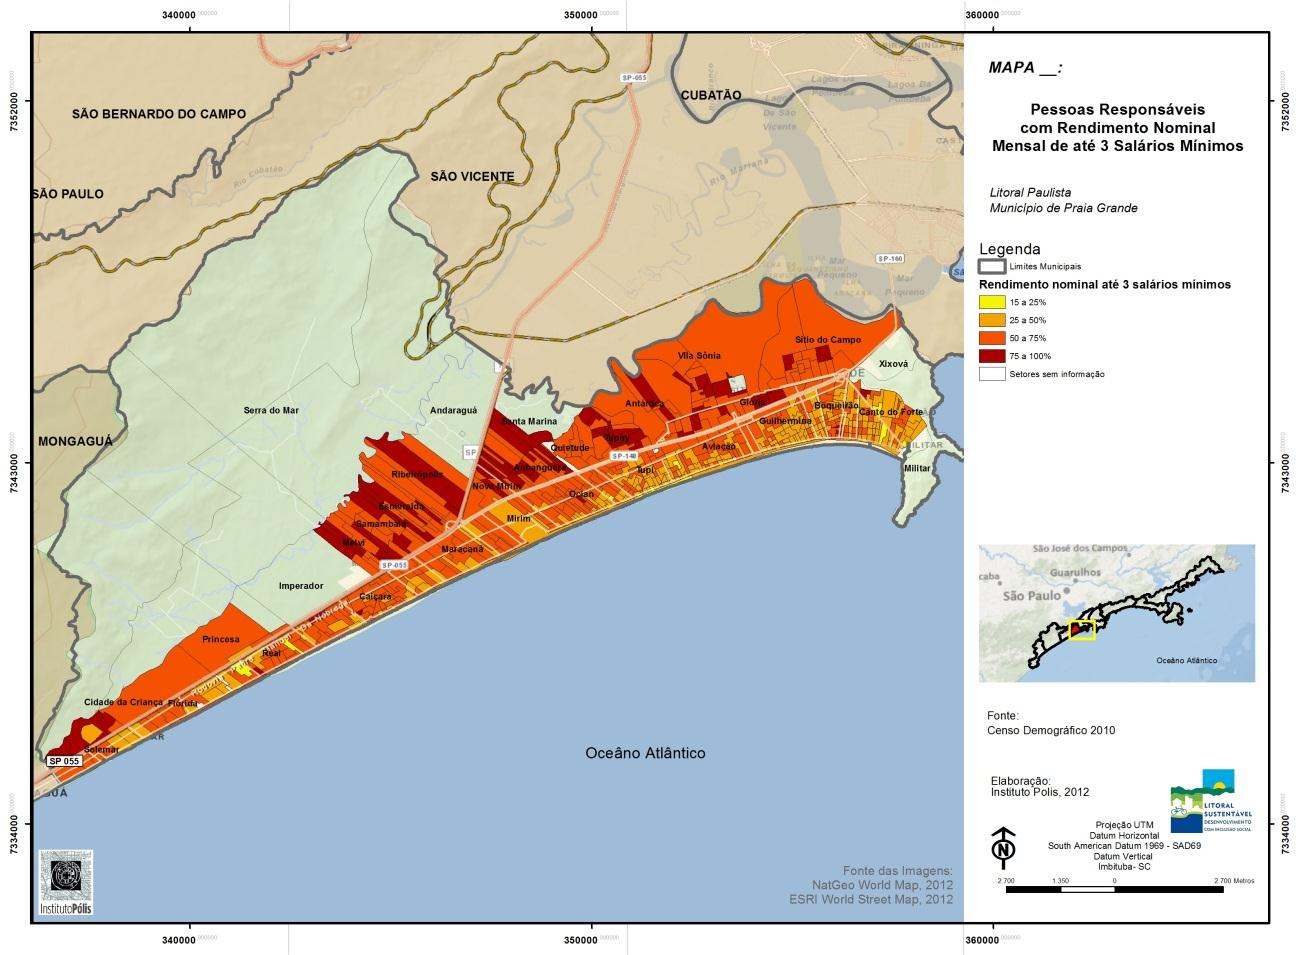
\includegraphics[width=20cm,height=20cm,keepaspectratio]{img/polis_3sm.png}
			\label{mapa_3sm}
			\legend{Fonte: \citeonline[p.26]{Polis2013a}}
		\end{figure}
	\end{landscape}

	\section{Habitação}
	
	% Acesso ao rascunho:
	% https://docs.google.com/document/d/1mFwaDl_7XzpnDU3eIPWPc0TjnHGwgI_xsTKqnn8OLM0/edit
	
	A dimensão habitacional é um ponto fulcral no ordenamento territorial da Praia Grande, visto que é esta que revela, territorialmente, a grande desigualdade originada e aprofundada pela vocação veranista do município. Isto é, as pessoas moram no cidade e relação deste ``morar'' com as dimensões ambientais, de mobilidade e acesso à infraestrutura é pautada pela renda que possuem, aprofundando disparidades.
	
	Praia Grande acompanha a tendência regional de aumento demográfico. Além da fixação da população, outras condições podem influenciar esse fenômeno: migração, natalidade ou efeitos da conjuntura econômica, o que gera maior demanda por infraestrutura e intensificar o adensamento desordenado em regiões em que já carecem de regularização fundiária e urbanística.
	
	Em análise realizada pelo Instituto Pólis, o município compunha um quadro junto a outras três cidades com déficit com taxas de crescimento deste acima de 100\% entre 2000 e 2010, evidenciando possíveis disputas por terra na região (vide Tabela \ref{tab_def_habit}).
	
	\begin{table}[h]
		\centering
		\caption{Déficit Habitacional RM Baixada Santista}
		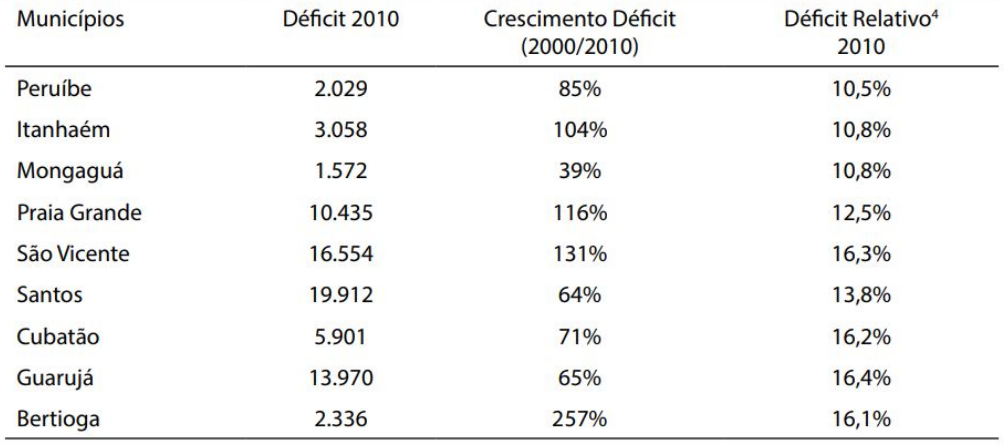
\includegraphics[width=1\textwidth]{img/tab_def_habit.png}
		\label{tab_def_habit}
		\legend{Elaboração: \citeonline[p.124-125]{rufino2015}. Fonte: \citeonline{fjp2013}}
	\end{table}
	
	As projeções realizadas pela \gls{agem} no âmbito do Plano Metropolitano de Desenvolvimento Estratégico da Baixada Santista corroboram tais informações. Indicam ainda a Praia Grande como um dos municípios mais críticos com relação ao déficit habitacional. A expansão dos assentamentos precários foi prevista pelo Plano, de forma generalizada na região. 
	
	A distribuição por área demonstra uma tendência de adensamento populacional em assentamentos precários, devido ao aumento do número de domicílios e aumento populacional, mas diminuição em área. Segundo o estudo do CEM/CEBRAP,  de 2010, 10,8\% das áreas mantiveram-se precárias, 7,2\% deixaram de ser precárias e 3,5\% tornaram-se precárias. Enquanto isso, em termos de população, 14,3\% mantiveram-se em situação de precariedade, 2,5\% deixaram de ser precárias e 5\% tornaram-se precárias.
	
	O município sofre ainda com grande inconsistência entre as básicas físicas e jurídicas do parcelamento, causando sobreposição de títulos, vazios não titulados, etc. \cite{pmpg2011b}\footnote{Trata-se do \gls{plhis} a referência \citeonline{pmpg2011b}}. A dificuldade generalizada em dimensionar os dados de déficit habitacional qualitativo e quantitativo configuram grave problema ao município e é refletida pela inconsistência das políticas voltadas para habitação e dificuldade em aplicação dos instrumentos. O Plano Local de Habitação de Interesse Social e Plano Diretor são insuficientes para o encaminhamento de soluções para o déficit municipal, priorizam a construção de unidades habitacionais e a regularização jurídica do domicílio.
	
	\subsection{Minha Casa Minha Vida}
	
	No que se refere às unidades construídas junto à Caixa, a efetividade do Programa Minha Casa Minha Vida com relação à diminuição do déficit habitacional na região é questionável, visto que atende, em grande parte, faixas 2 e 3, que possuem maior renda familiar (vide Tabela \ref{tab_pmcmv}).
	
	\begin{table}[h]
		\centering
		\caption{Produção do PMCMV na \gls{rmbs}, segundo fases e faixas de renda}
		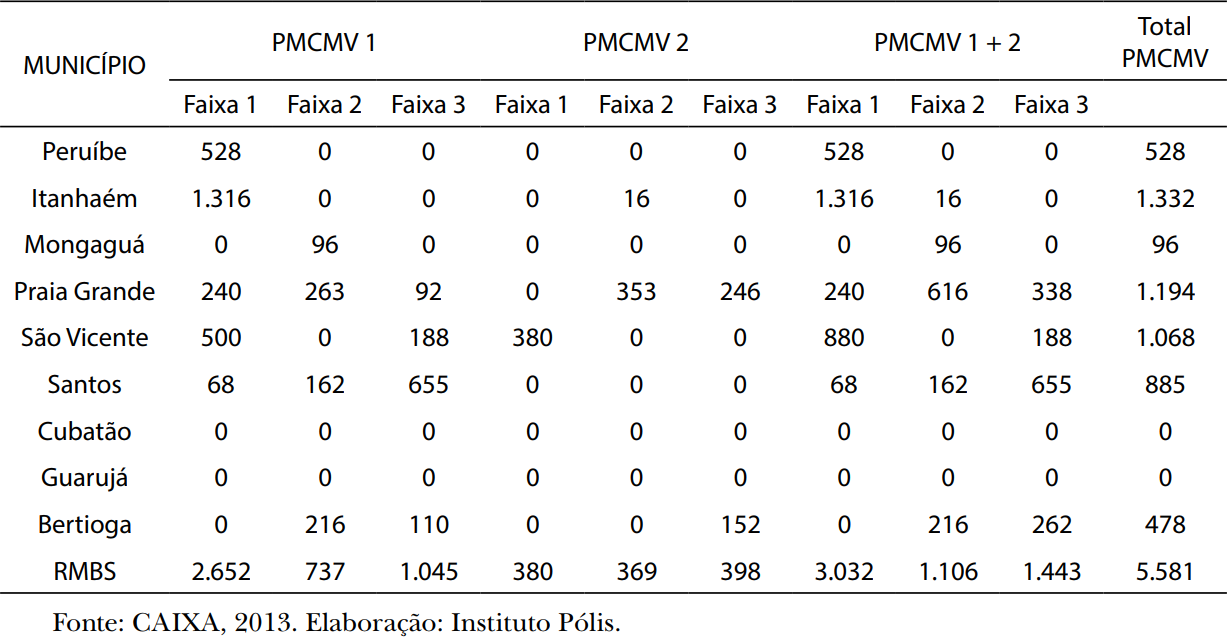
\includegraphics[width=1\textwidth]{img/tab_pmcmv.png}
		\label{tab_pmcmv}
		\legend{Extraído de: \citeonline[p.115]{amore2015}}
	\end{table}
	
	Durante a elaboração deste relatório, Praia Grande foi selecionada para a construção de 972 moradias de faixa 1 (renda familiar de até R\$ 1.800,00) em terrenos doados pela prefeitura, distribuídos entre os bairros Antártica e Esmeralda \cite{pmpg2017l}, em áreas previstas como Zonas Especiais de Interesse Social. Espera-se das unidades previstas para o Balneário Maxland, na Vila Antártica, que atenuem as pressões exercidas pela ocupação irregular às áreas do Parque do Piaçabuçu. No entanto, no geral, a localização das áreas delimitadas para a implantação do Programa reforçam a lógica segregacionista do município, consolidando habitações em áreas de infraestrutura precária, acesso dificultoso aos equipamentos disponíveis no município e com potencial de expansão muito limitado.
	
	% Parágrafo abaixo estava em vermelho no Docs
	No limite, a aplicação dos instrumentos do Estatuto da Cidade para um ordenamento territorial que tenha como princípios básicos a justa distribuição de ônus e bônus dos processos de desenvolvimento econômico contraria a vocação da cidade. Realizar a manutenção dessa vocação significa reafirmar e intensificar desigualdades.	
	
	\subsection{Assentamentos precários}
	
	O Censo 2010 do \gls{ibge} aponta a existência de pelo menos seis assentamentos precários na cidade, relativamente próximos entre si. São eles o Jardim Marília, Núcleo Caieiras, Núcleo Celimar, Núcleo Maxland, Núcleo Mirim e Núcleo Piratas, manifestando o padrão de renda. 
	
	As Zonas Especiais de Interesse Social (\gls{zeis}) estabelecidas pelo \gls{pde} indicam áreas para regularização fundiária (ZEIS 1). São áreas de grande densidade demográfica, ocupadas por população de baixa-renda e em assentamentos irregulares. Estão concentradas entre os bairros Melvi, Esmeralda, Ribeirópolis, Nova Mirim, Anhanguera, Quietude e Tupiry, em área predominantemente residencial, limite com o Parque do Piaçabuçu e área de uso diversificado de porte regional (que abrigará o grande empreendimento Complexo Andaraguá).
	
	Os bairros Melvi (ZEIS 2) e Cidade da Criança (ZEIS 1) apresentam ocupações dispersas ao longo do arruamento e necessidade de remoções pontuais, devido a área de risco.
	
	\begin{figure}[h]
		\centering
		\caption{Identificação de assentamentos precários (azul claro) em Praia Grande}
		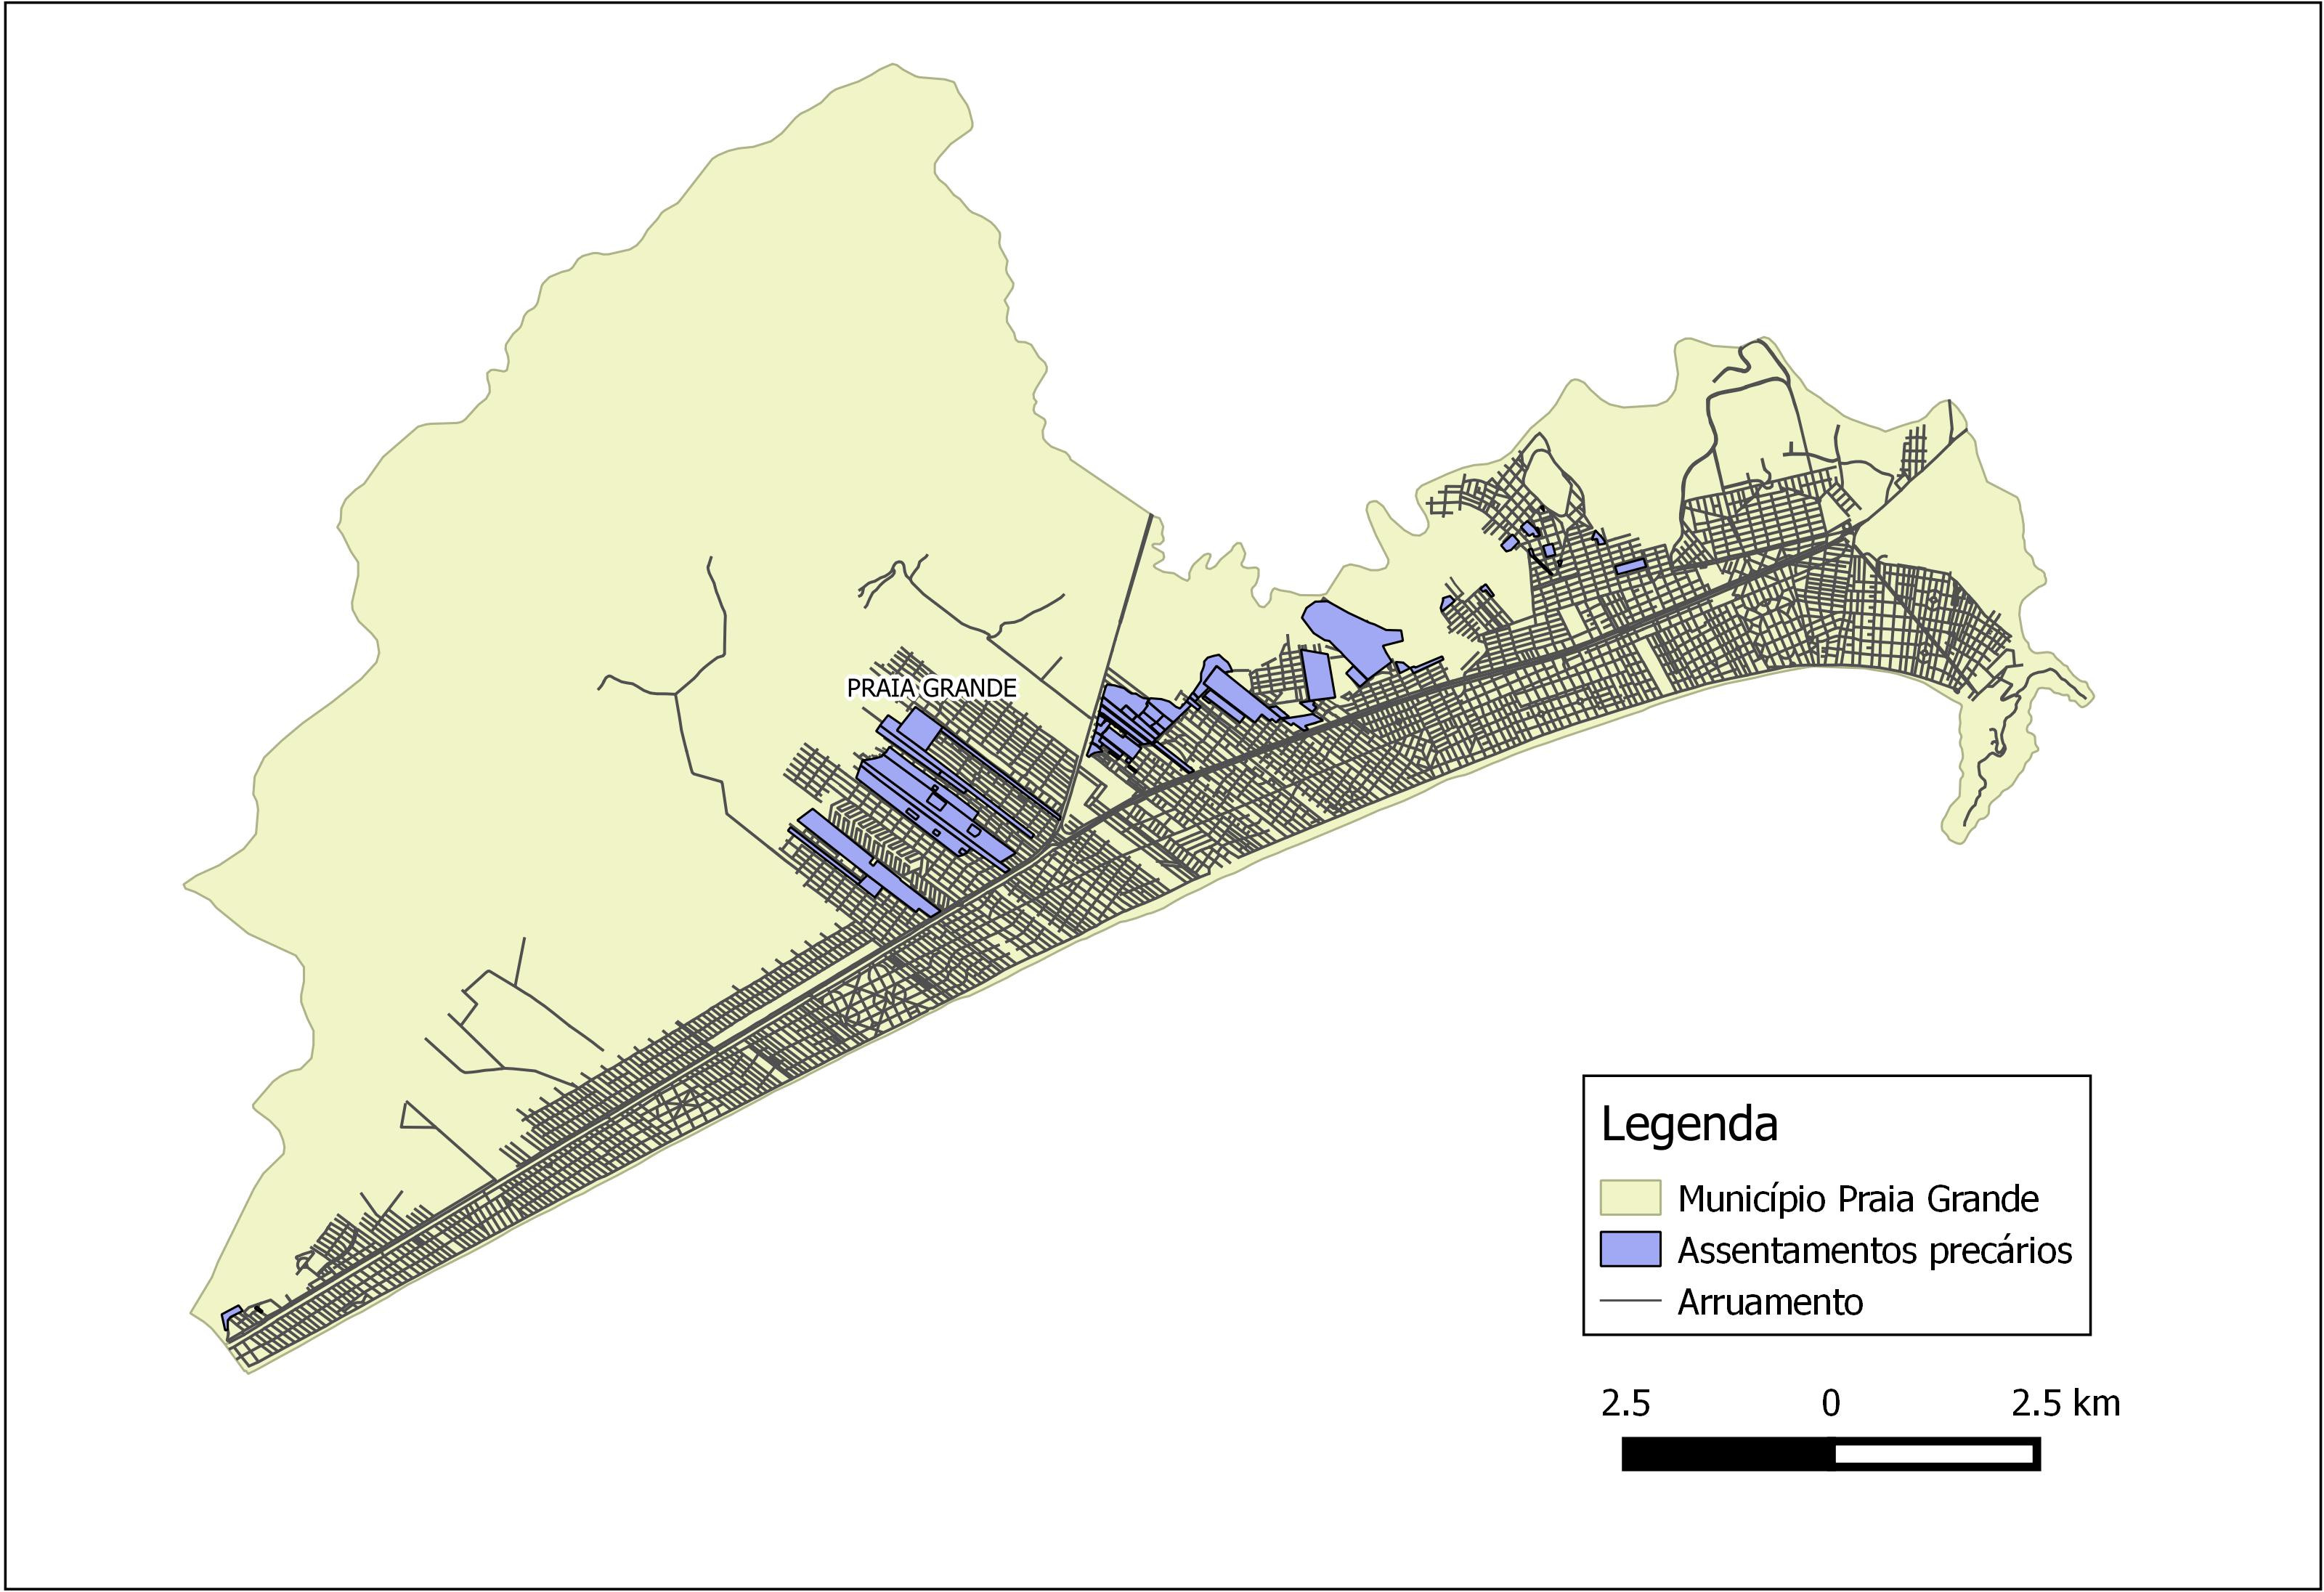
\includegraphics[width=1\textwidth]{img/Assentamentos_precarios_atualizado.jpg}
		\label{mapa_favelas}
		\legend{Elaboração própria}
	\end{figure}
	
	Há ainda ZEIS 1 dispersas entre os bairros Antártica e Vila Sônia, também em área limítrofe ao Parque do Piaçabuçu. As ZEIS 1 indicam interesse geral em manter a população no local e promover regularização fundiária e urbanística. Mais informações acerca das \gls{zeis} estão dispostas na seção \ref{ord_territorial}.
	
	Finalmente, é possível identificar que as áreas com assentamentos precários também se distribuem na parte norte da rodovia Padre Manoel da Nóbrega.
	
	\section{Sistema de mobilidade}
	% Minha parte
	
	O município está implementando um plano de mobilidade próprio, definido publicamente no sítio oficial conforme citação abaixo.
	
	\begin{citacao}		
		O PlanMobPG vai abranger todo o território do Município e seu objetivo geral é desenvolver propostas de políticas e ações para permitir o acesso aos sistemas de circulação: ruas, calçadas, linhas de ônibus, táxis, ciclovias, terminais de integração, estacionamentos e todos os demais serviços que visem transportar pessoas e mercadorias.
		
		Sua elaboração começou em 2013, quando foi iniciada a Consulta Pública sobre o tema, nos bairros da cidade.
		
		\cite{pmpg2017a}
	\end{citacao}
	
	O plano de mobilidade é considerado um plano setorial, convencionado pelo poder público como um instrumento para implementação do Plano Diretor, detalhando as diretrizes gerais por ele estabelecidas. Considerando o Plano Nacional de Mobilidade Urbana, trata-se de um plano municipal obrigatório devido ao fato de o município apresentar mais de 20 mil habitantes \cite[Art. 24\textordmasculine, \S 1\textordmasculine]{gf2012a}.
	
	A administração municipal define ainda que o plano de mobilidade ``tem por objetivo contribuir para o acesso universal à cidade, por meio do planejamento e da gestão democrática do Sistema Nacional de Mobilidade Urbana'' \cite{pmpg2017b}, bem como define que o Sistema de Mobilidade Urbana, ``é o conjunto organizado e coordenado dos modos de transporte, de serviços e de infraestruturas, que garante os deslocamentos de pessoas e cargas no território do Município'' \cite{pmpg2017b}.

	\begin{figure}[h]
		\centering
		\caption{Diagrama do PLANMOBPG}
		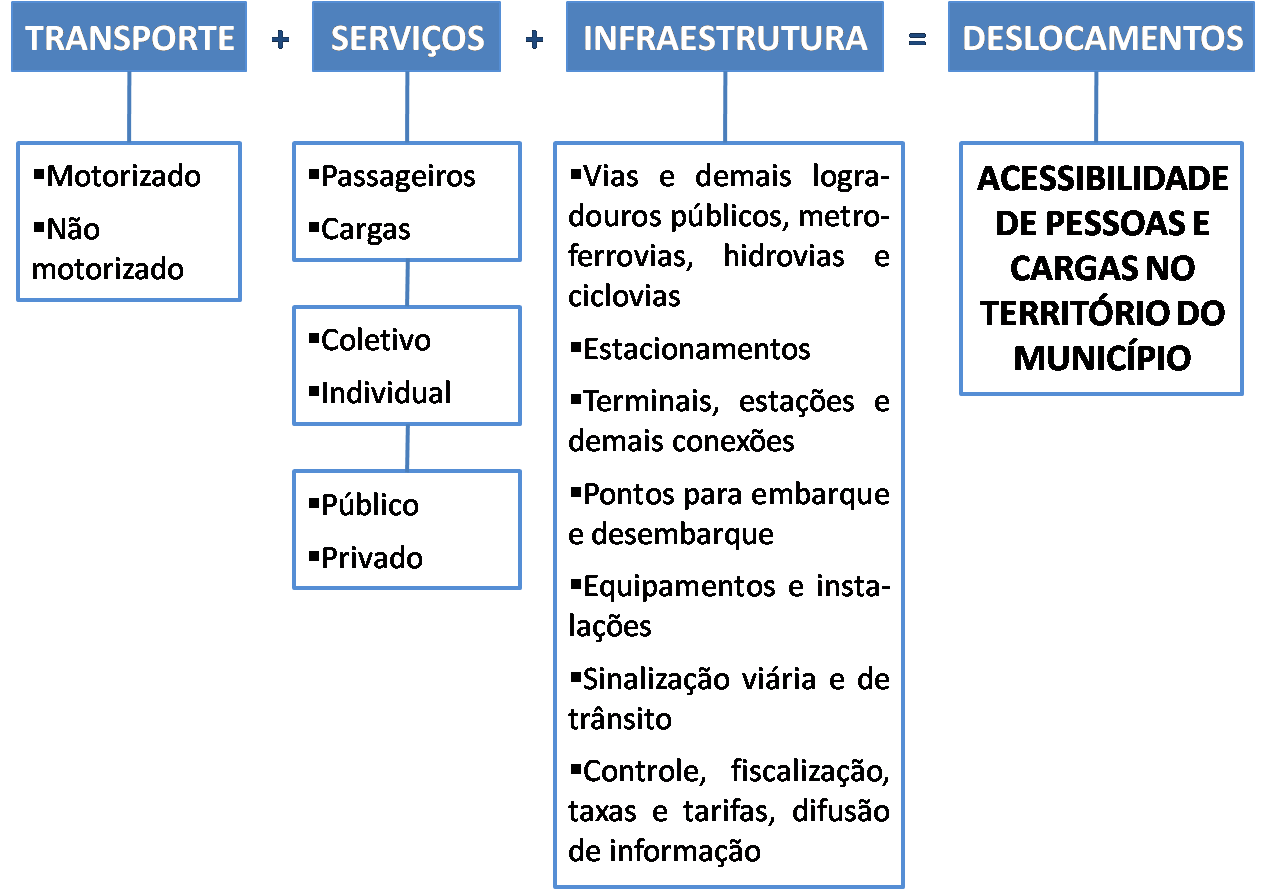
\includegraphics[width=1\textwidth]{img/planmob_apresentacao.png}
		\label{diagrama_planmob}
		\legend{Fonte: \citeonline{pmpg2017b}}
	\end{figure}
	
	\subsection{Transporte coletivo municipal}
	
	Considerando a Política Nacional de Mobilidade Urbana \cite[Art. 4\textordmasculine, inciso VI]{gf2012a}, as linhas municipais de ônibus de Praia Grande estão qualificadas como: ``transporte público coletivo: serviço público de transporte de passageiros acessível a toda a população mediante pagamento individualizado, com itinerários e preços fixados pelo poder público''.
	
	A partir do sítio da Viação Piracicabana na Internet \cite{piracicabana2017a}, foram identificadas as seguintes linhas municipais de transporte urbano sobre pneus por meio de ônibus:
	
	\begin{itemize}
		\item Linha 11PR;
		\item Linha 12CO;
		\item Linha 13TR;
		\item Linha 15SO;
		\item Linha 17SA;
		\item Linha 22ME;
		\item Linha 30JT;
		\item Linha 33MA;
		\item Linha 94BF;
		\item Linha 95CF;
		\item Linha 96CF;
		\item Linha 97SH;
		\item Linha 98JP;
		\item Linha CBS.
	\end{itemize}

	O município também fornece um mapa das linhas municipais de ônibus como parte dos dados públicos do PLANMOBPG. Vide figura \ref{mapa_onibusmuni}.
	
	\begin{landscape}
		\begin{figure}[p]
			\centering
			\caption{Itinerário das Linhas Municipais}
			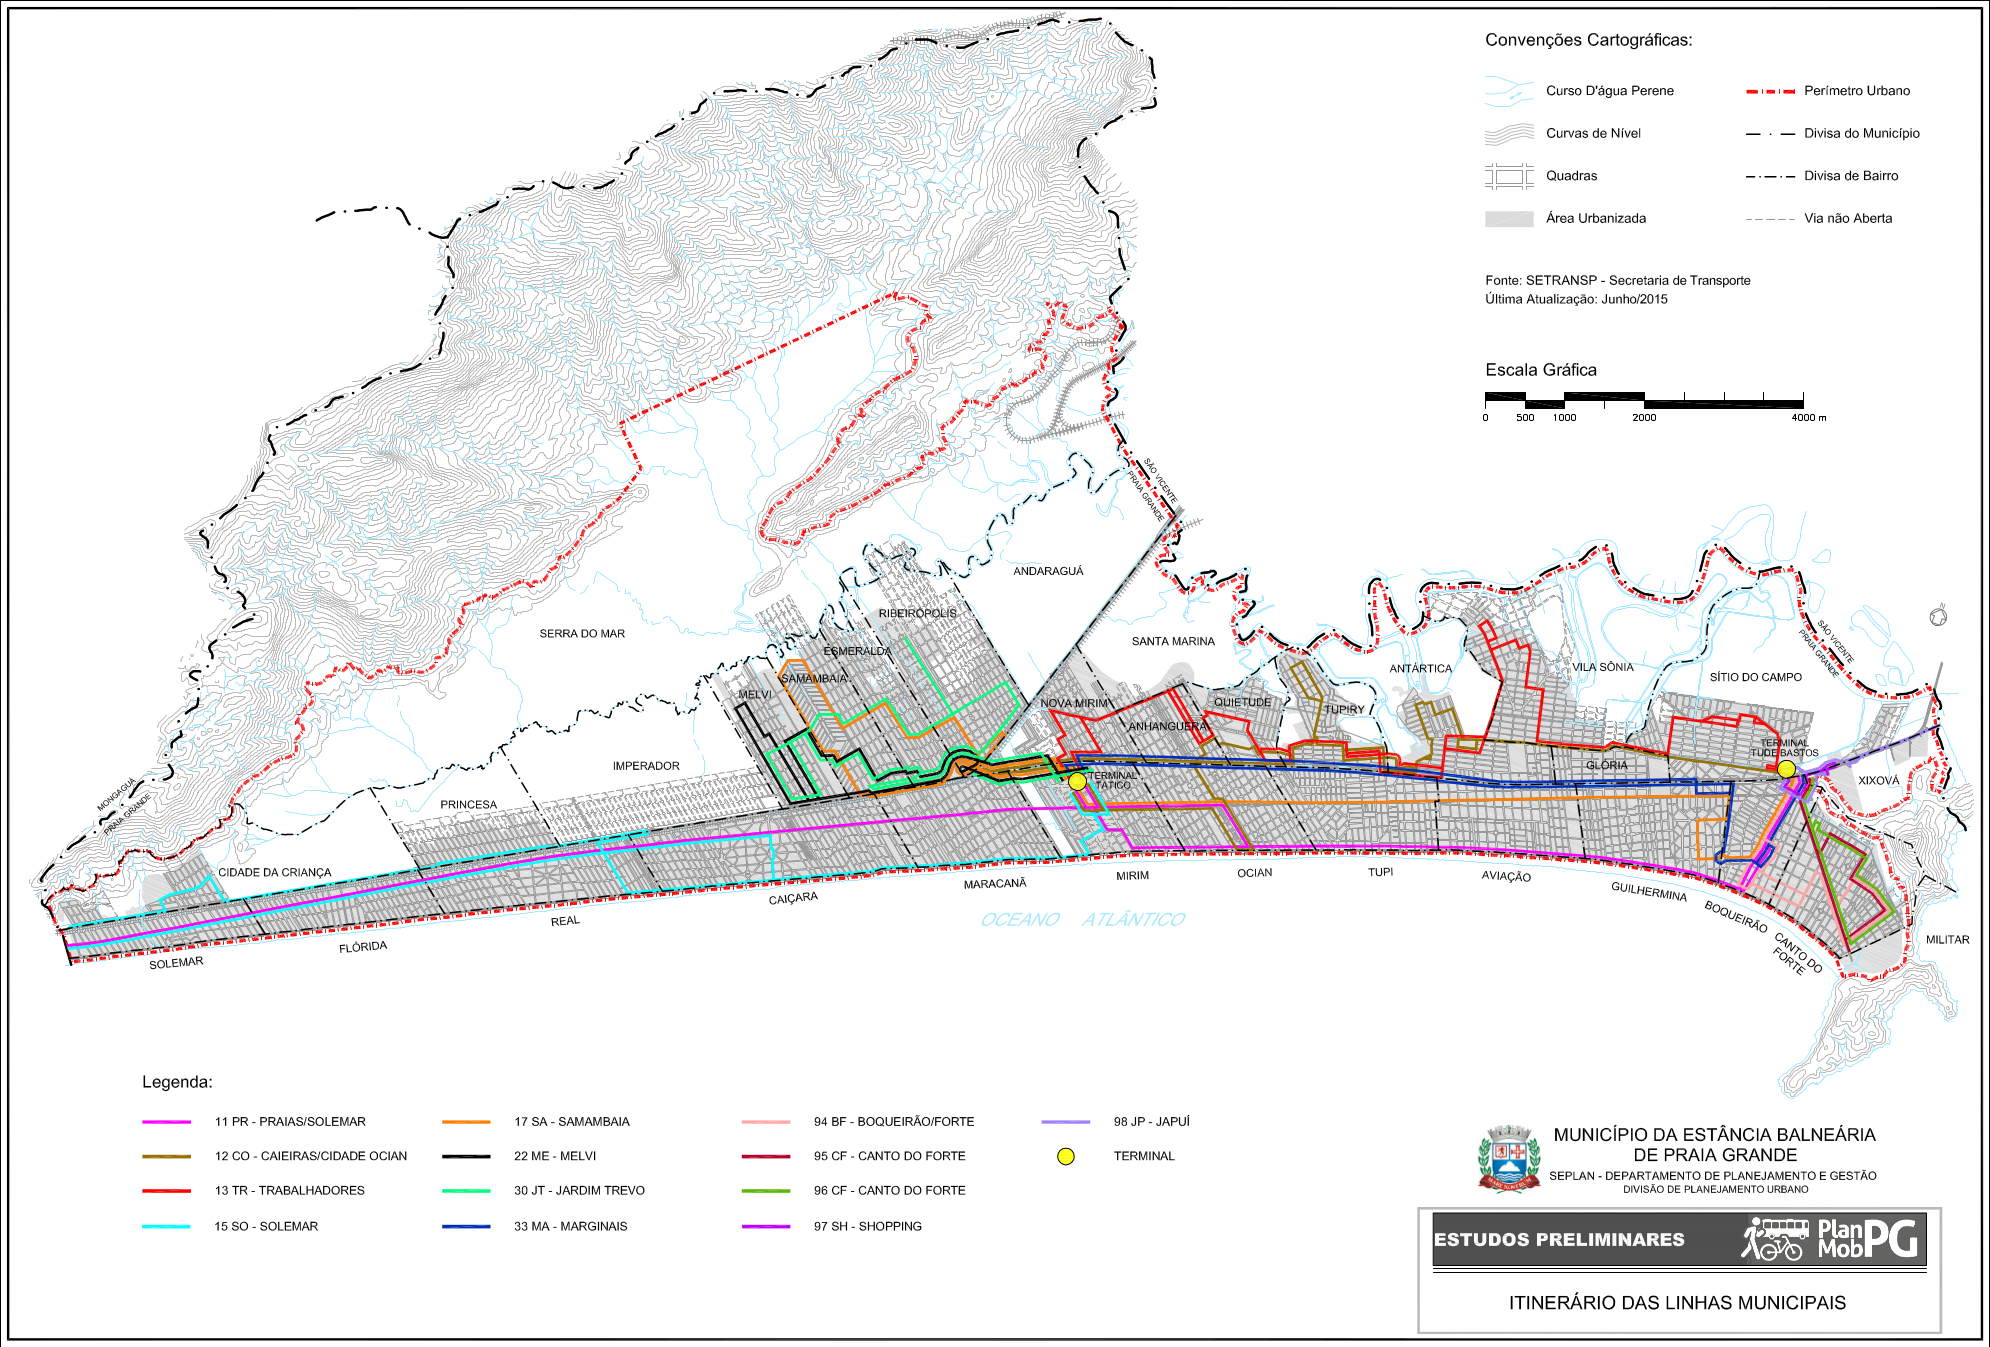
\includegraphics[width=22cm,height=22cm,keepaspectratio]{img/Itinerario_das_Linhas_Municipais.png}
			\label{mapa_onibusmuni}
			\legend{Fonte: \citeonline{pmpg2015a}}
		\end{figure}
	\end{landscape}
	
	\subsection{Transporte coletivo intermunicipal}
	
	Conforme a Política Nacional de Mobilidade, cabe ao Governo do Estado de São Paulo a responsabilidade no tocante ao transporte de caráter intermunicipal (metropolitano):
	
	\begin{citacao}
		São atribuições dos Estados: 
		
		I - prestar, diretamente ou por delegação ou gestão associada, os serviços de transporte público coletivo intermunicipais de caráter urbano, em conformidade com o \S 1\textordmasculine do art. 25 da Constituição Federal;
		
		(\dots)
		
		\cite[Art. 17\textordmasculine, inciso I]{gf2012a}
	\end{citacao}
	
	Considerando o arcabouço institucional do Governo do Estado de São Paulo, a \gls{emtu} passou a atuar na Região Metropolitana da Baixada Santista conforme o Decreto N\textordmasculine 45.983, de 8 de agosto de 2001:
	
	\begin{citacao}
		(\dots) Aplicam-se concomitantemente na Região Metropolitana da Grande São Paulo, na Região Metropolitana da Baixada Santista e na Região Metropolitana de Campinas, no que couber, o disposto no Decreto n\textordmasculine 24.675, de 30 de janeiro de 1986, alterado pelo Decreto n\textordmasculine 27.436, de 7 de outubro de 1987, e pelo Decreto n\textordmasculine 38.352, de 26 de janeiro de 1994, que regulamentam os Serviços Metropolitanos de Transporte Coletivo Regular de Passageiros por Ônibus, bem como o Decreto n\textordmasculine 19.835, de 29 de outubro de 1982, alterado pelo Decreto n\textordmasculine 28.478, de 3 de junho de 1988 e Decreto n\textordmasculine 36.963, de 23 de junho de 1993, que regulamentam os Serviços de Transporte Coletivo de Passageiros de Interesse Metropolitano, sob o regime de fretamento.
		
		(\dots)
		
		\cite[Art. 2\textordmasculine]{gesp2001a}
	\end{citacao}

	\begin{figure}[p]
		\centering
		\caption{Ciclovia na região da Av. dos Trabalhadores}
		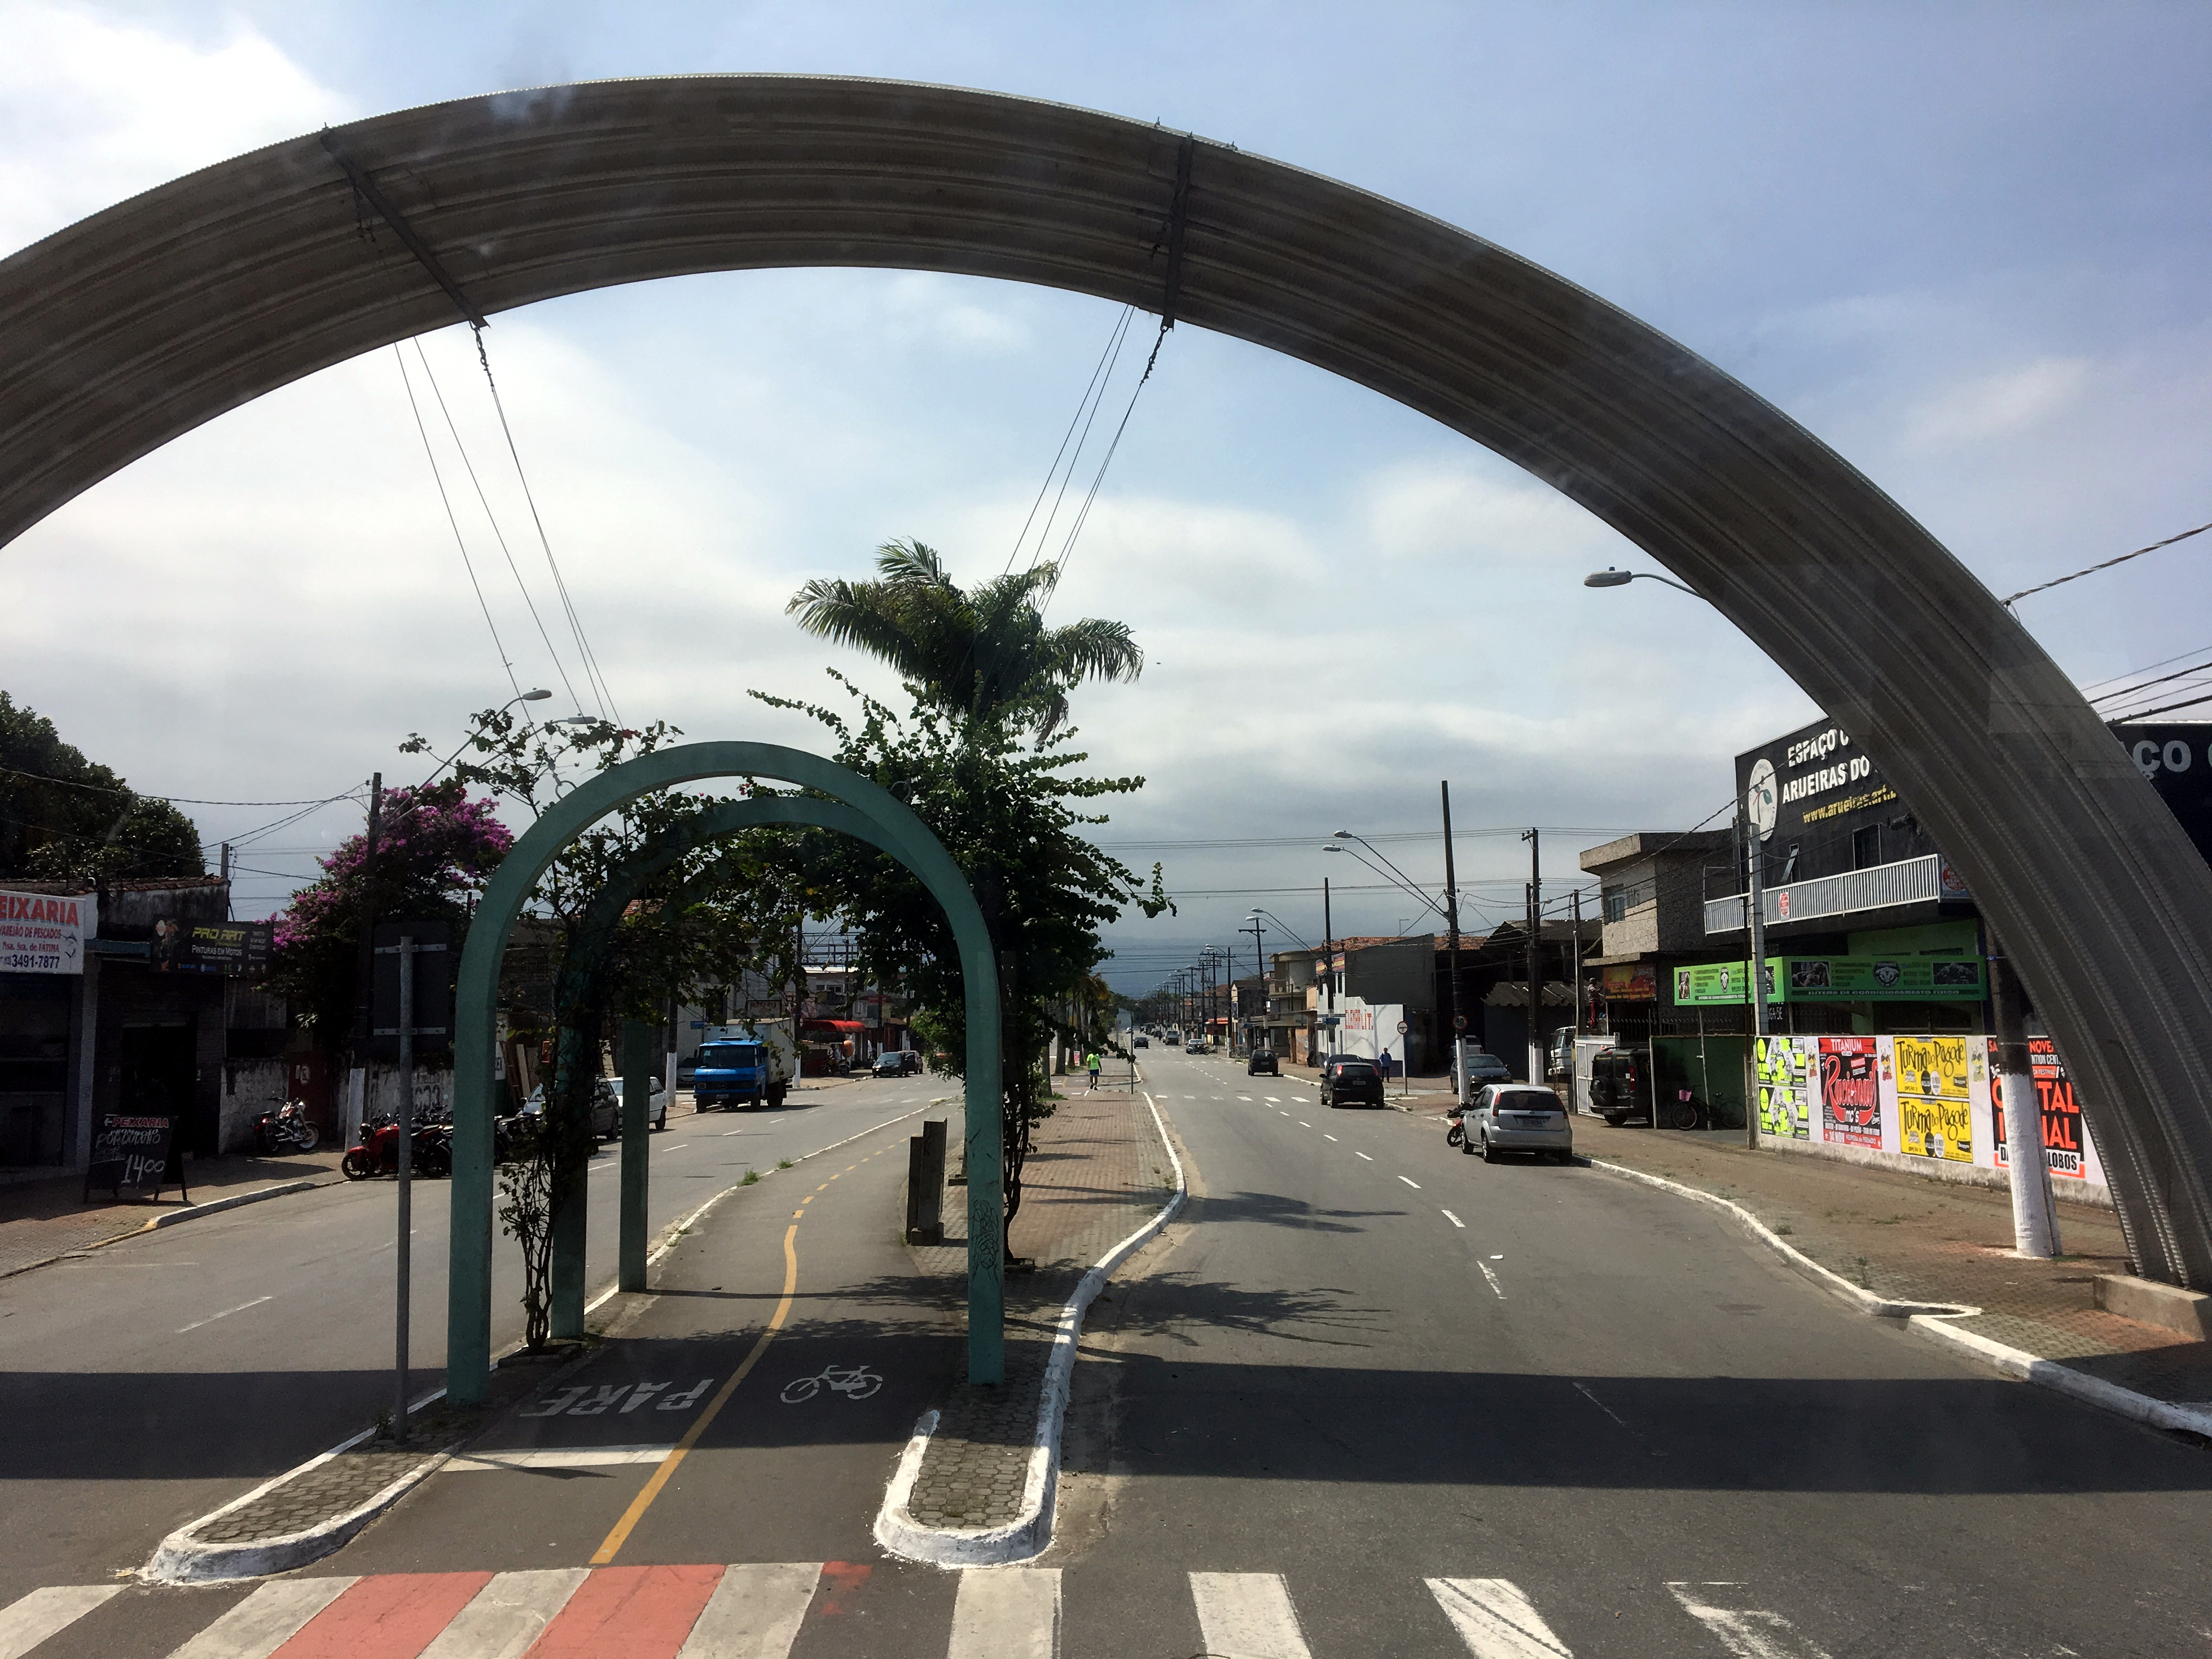
\includegraphics[width=0.5\textwidth]{img/IMG_2029.JPG}
		\legend{Elaboração própria}
	\end{figure}
	
	\begin{figure}[p]
		\centering
		\caption{Ciclovia na orla da praia, bairro Ocian}
		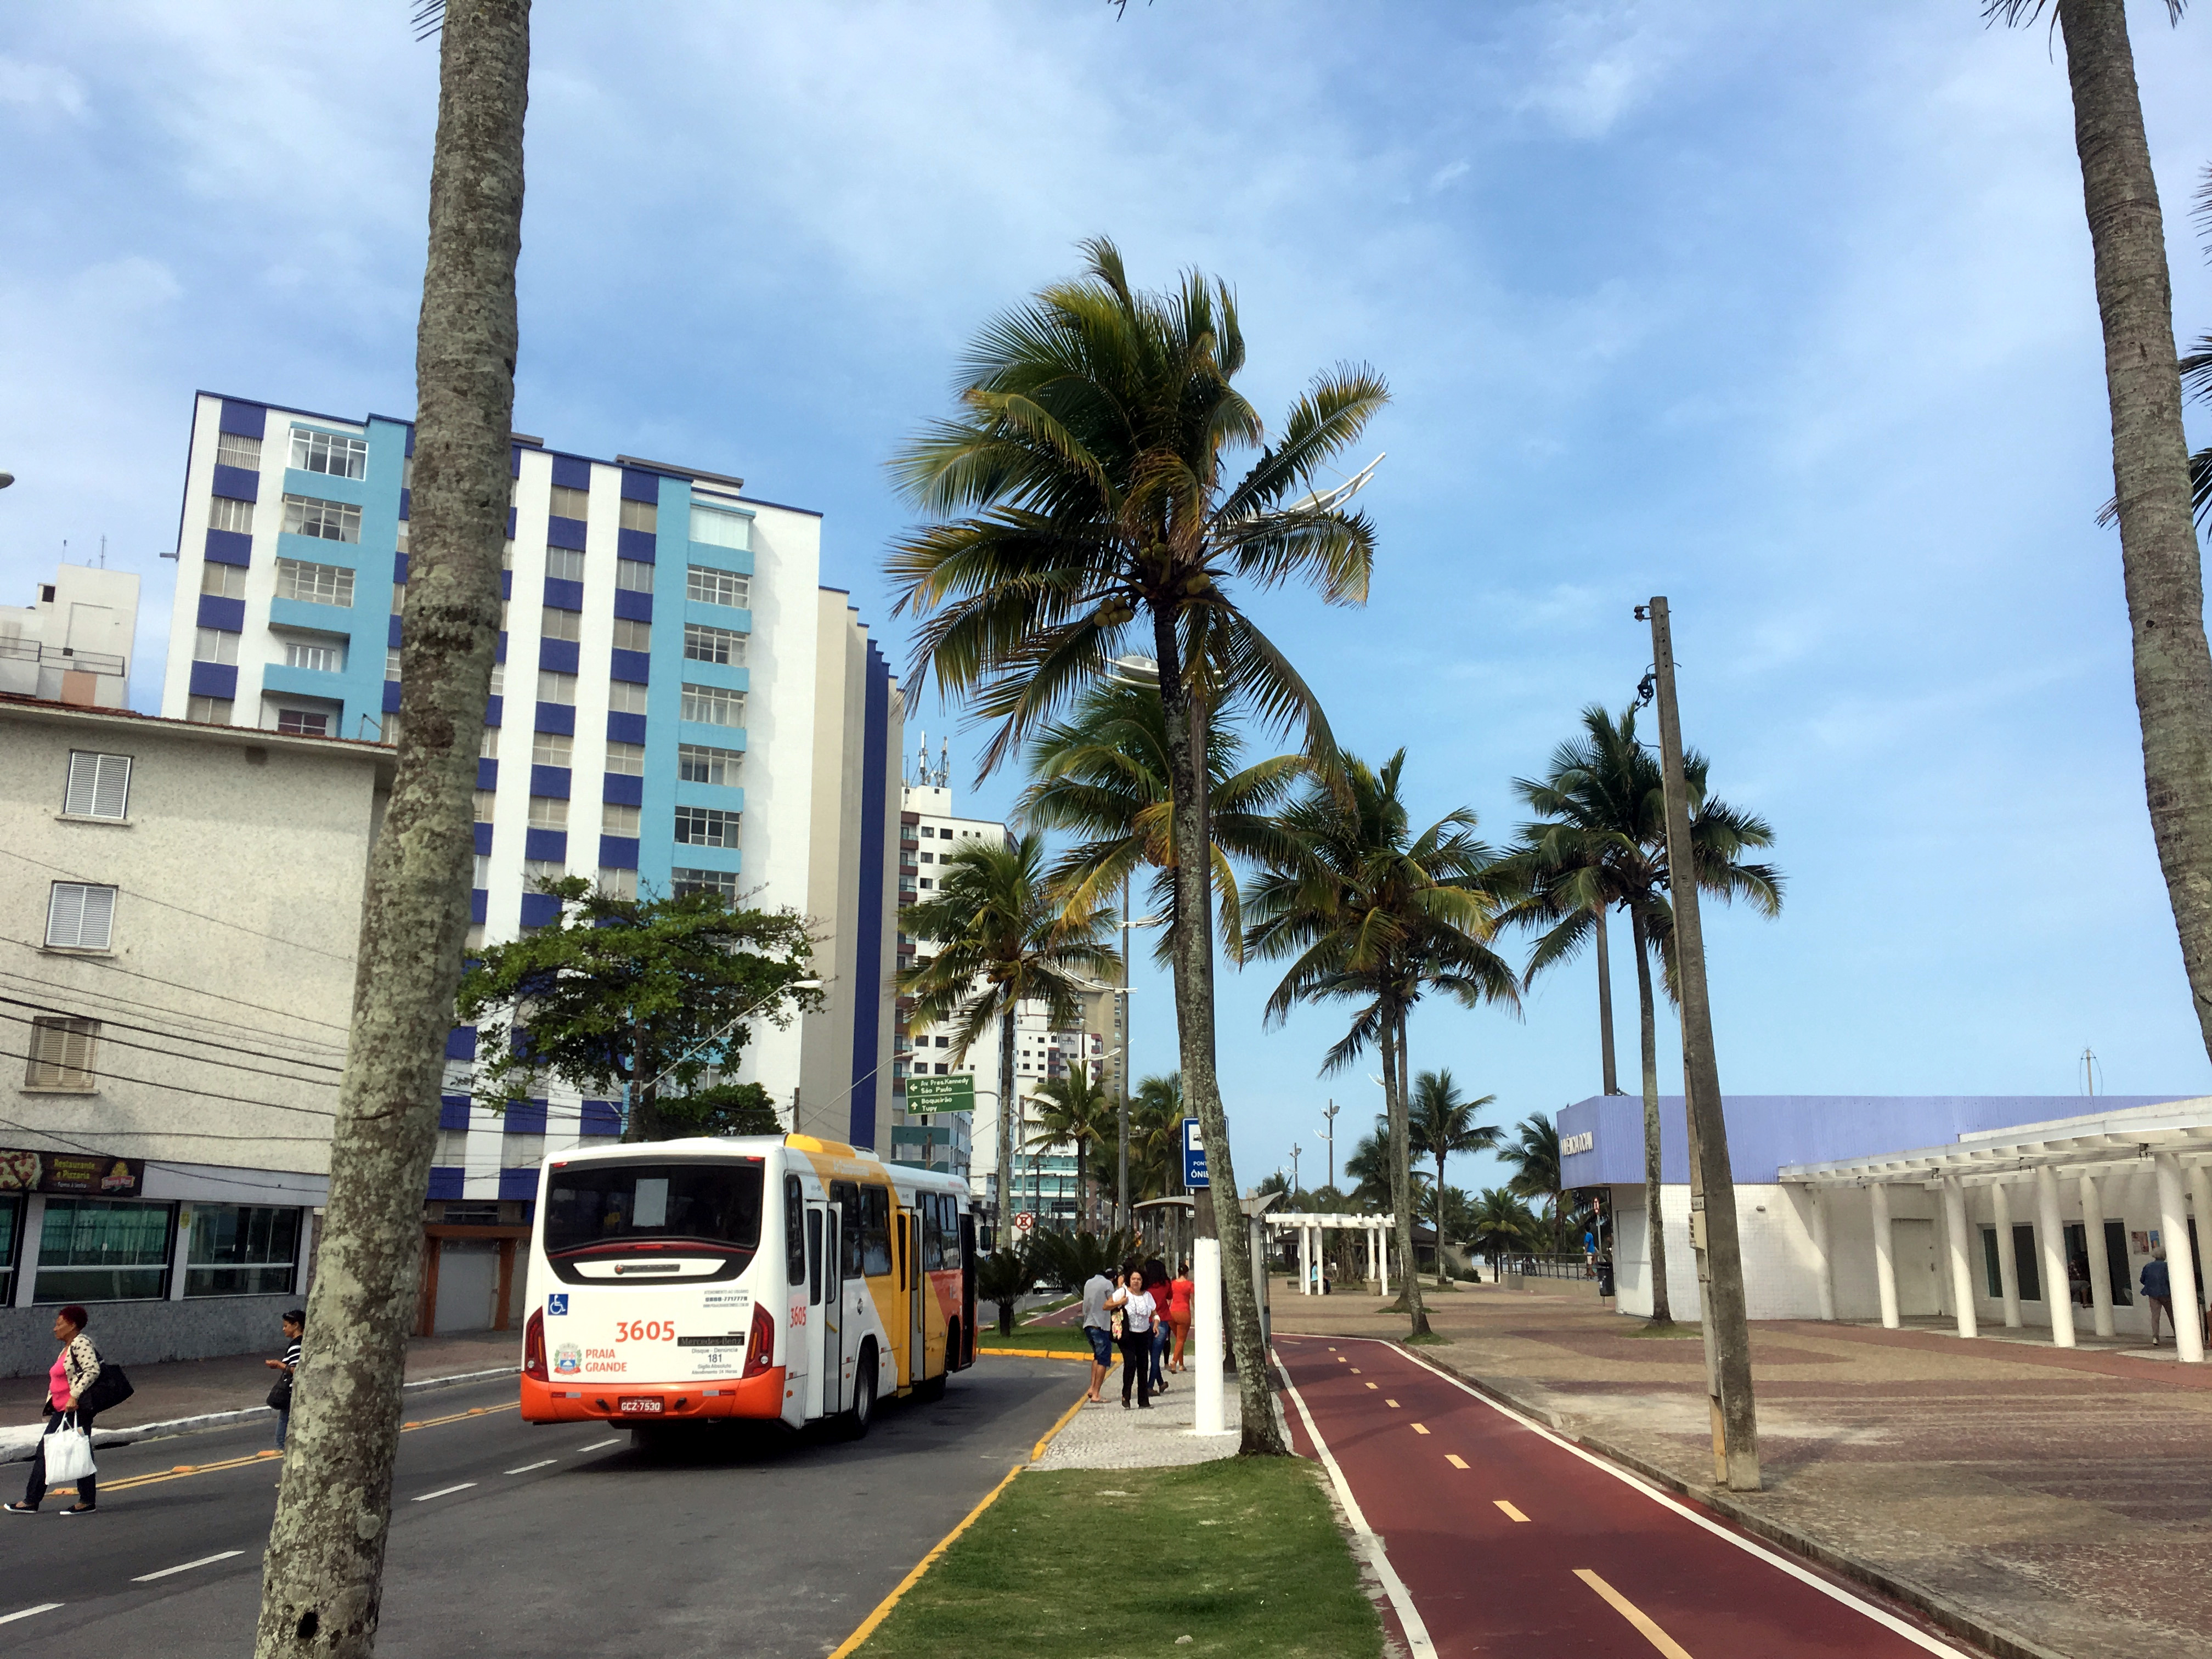
\includegraphics[width=0.5\textwidth]{img/IMG_2282.JPG}
		\legend{Elaboração própria}
	\end{figure}
	
	\begin{figure}[p]
		\centering
		\caption{Ciclovia da orla sendo utilizada por dois ciclistas}
		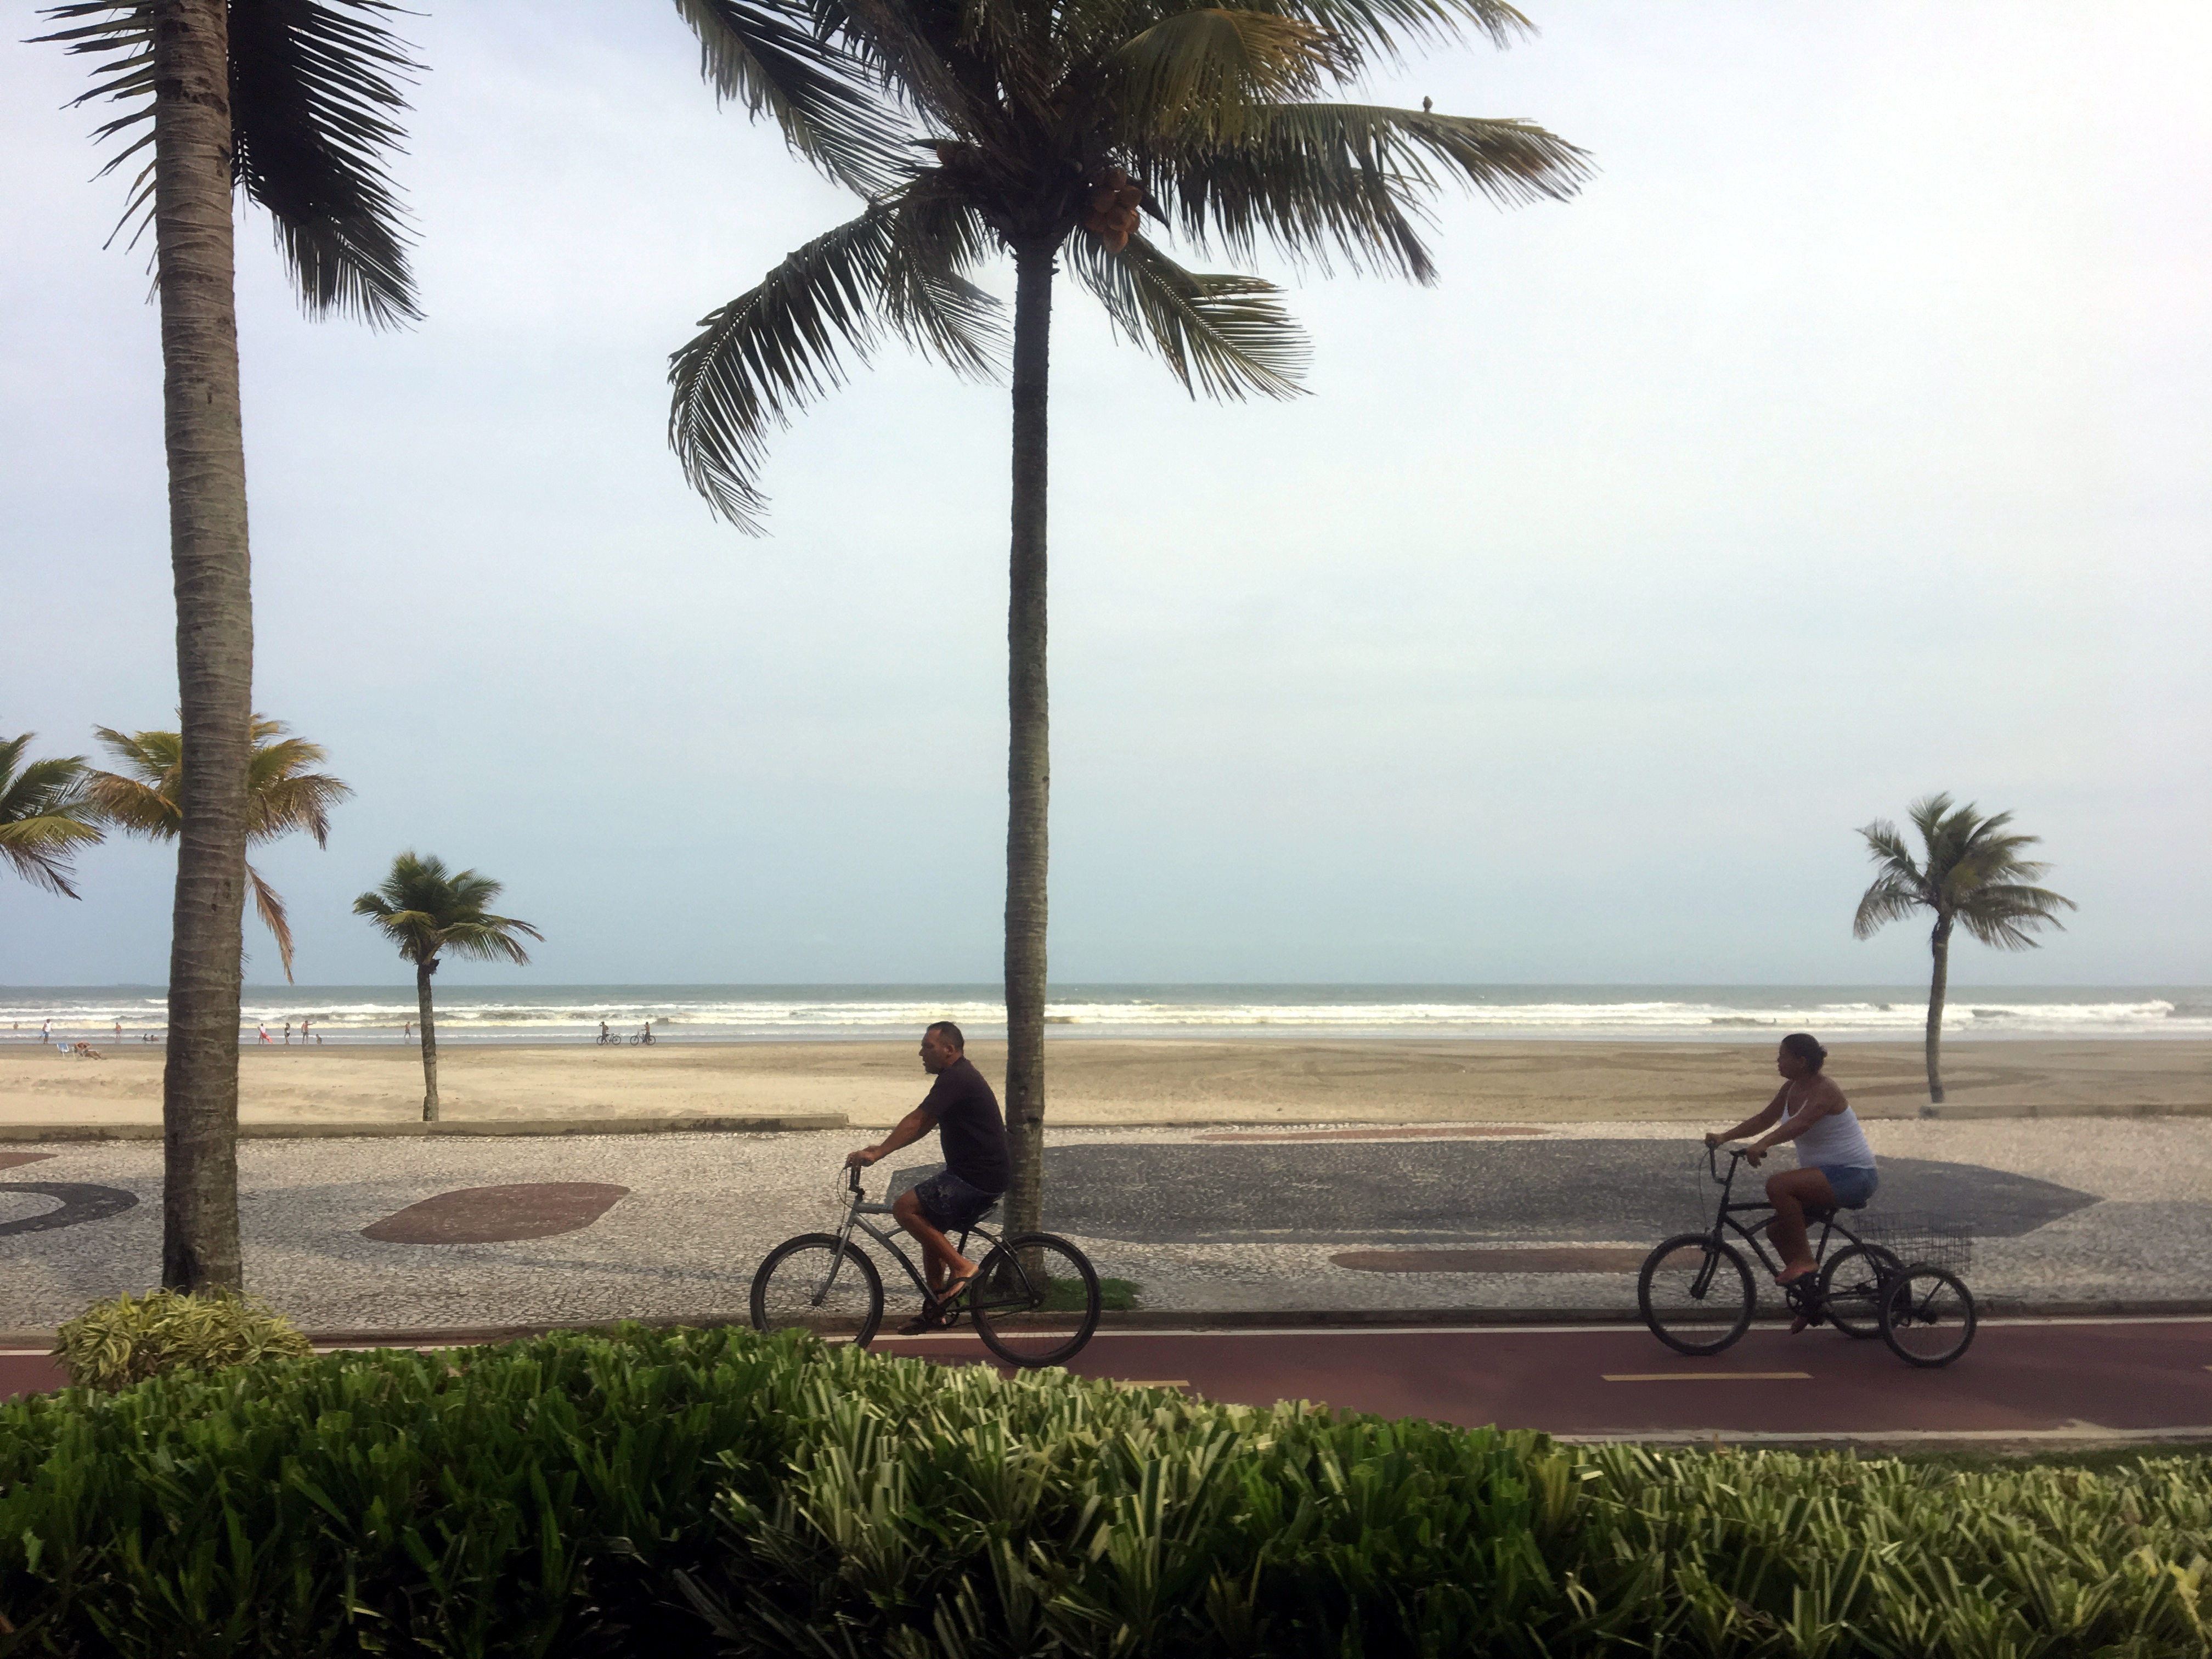
\includegraphics[width=0.5\textwidth]{img/IMG_2354.JPG}
		\legend{Elaboração própria}
	\end{figure}
	
	\subsection{Transporte coletivo de caráter estrutural} \label{transp_estrutural}
	
	A conceituação do transporte como sendo de caráter de estrutural (referindo-se especificamente ao transporte sobre trilhos) pode ser pensada a partir de \apudonline[p.13]{Merlin1991a}{daLuz2010a}: ``o autor afirma que os tempos dos retornos dos investimentos feitos na ferrovia são normalmente diferentes daqueles de outros investimentos e, principalmente, as suas características influem na localização das demais atividades humanas, modificam a paisagem de forma indelével, mesmo após seu abandono''.
	
	No âmbito de suas atribuições a EMTU tem implantado um sistema de \gls{vlt} em Santos e São Vicente, sendo prevista uma extensão do sistema com modo \gls{brt} em Praia Grande. Segundo \citeonline{EMTU2017a}, ``o  primeiro trecho do VLT, com 11,5km de extensão foi entregue à população no dia 31/01/2017, ligando o Terminal Barreiros, em São Vicente, à Estação Porto, em Santos. A operação parcial no trecho começou em abril de 2015''.
	
	\begin{landscape}
		\begin{figure}[p]
			\centering
			\caption{Mapa elucidando as primeiras fases de implantação do \gls{vlt}}
			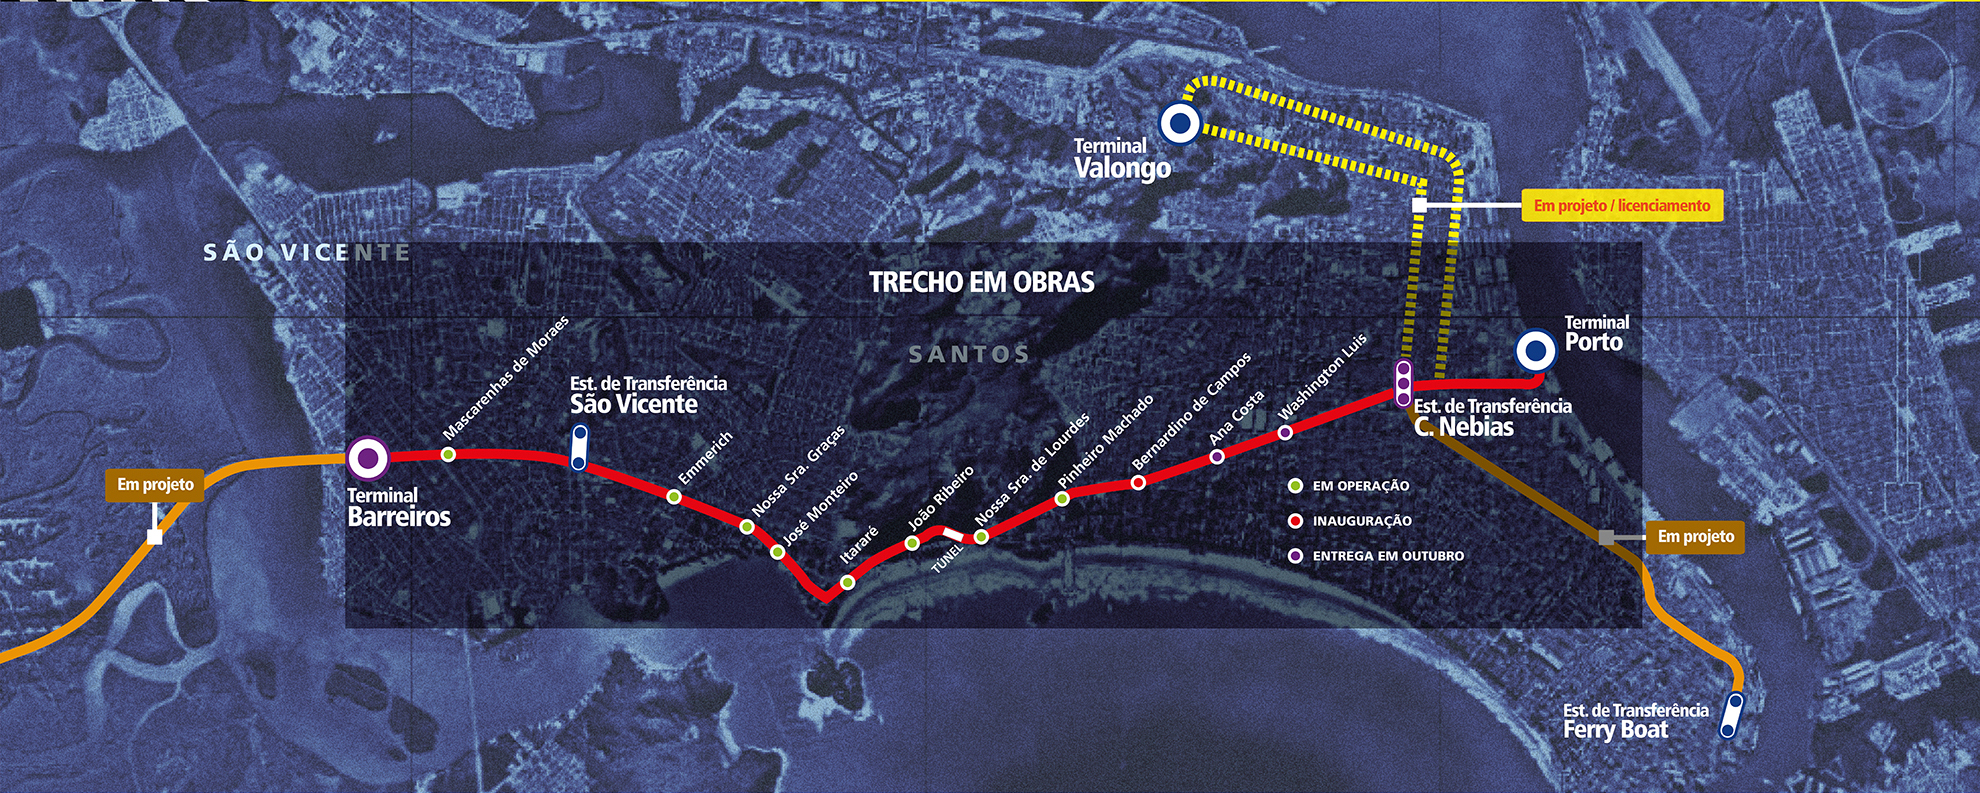
\includegraphics[width=25cm,height=25cm,keepaspectratio]{img/tracado-vlt.jpg}
			\label{mapa_vlt}
			\legend{Fonte: \citeonline{EMTU2017a}}
		\end{figure}
	\end{landscape}
	
	Durante a visita de campo guiada, as funcionárias da administração municipal comentaram que o atual prefeito tem solicitado a extensão do \gls{vlt} até o Terminal Rodoviário e Urbano Francisco Gomes da Silva 'Tatico', no entanto, por se tratar de um sistema que reaproveitou o leito do antigo \gls{tim} (operado pela \gls{fepasa} e extinto pela \gls{cptm}), o pleito exigiria a ampliação do \gls{vlt} em São Vicente até Samaritá, e, em seguida, por toda a Via Expressa Sul a partir da Rodovia Padre Manoel da Nóbrega (SP-55).
	
	Vale apontar que permanece subutilizado o leito do antigo Ramal de Juquiá da \gls{fepasa} ao longo da Rodovia Padre Manoel da Nóbrega (SP-55), sendo identificado pelo grupo um antigo cruzamento (ainda com a sinalização ferroviária) e em via singela.

	\begin{figure}[!htb]
		\centering
		\caption{Cruzamento em nível do Ramal de Juquiá no dia da visita de campo}
		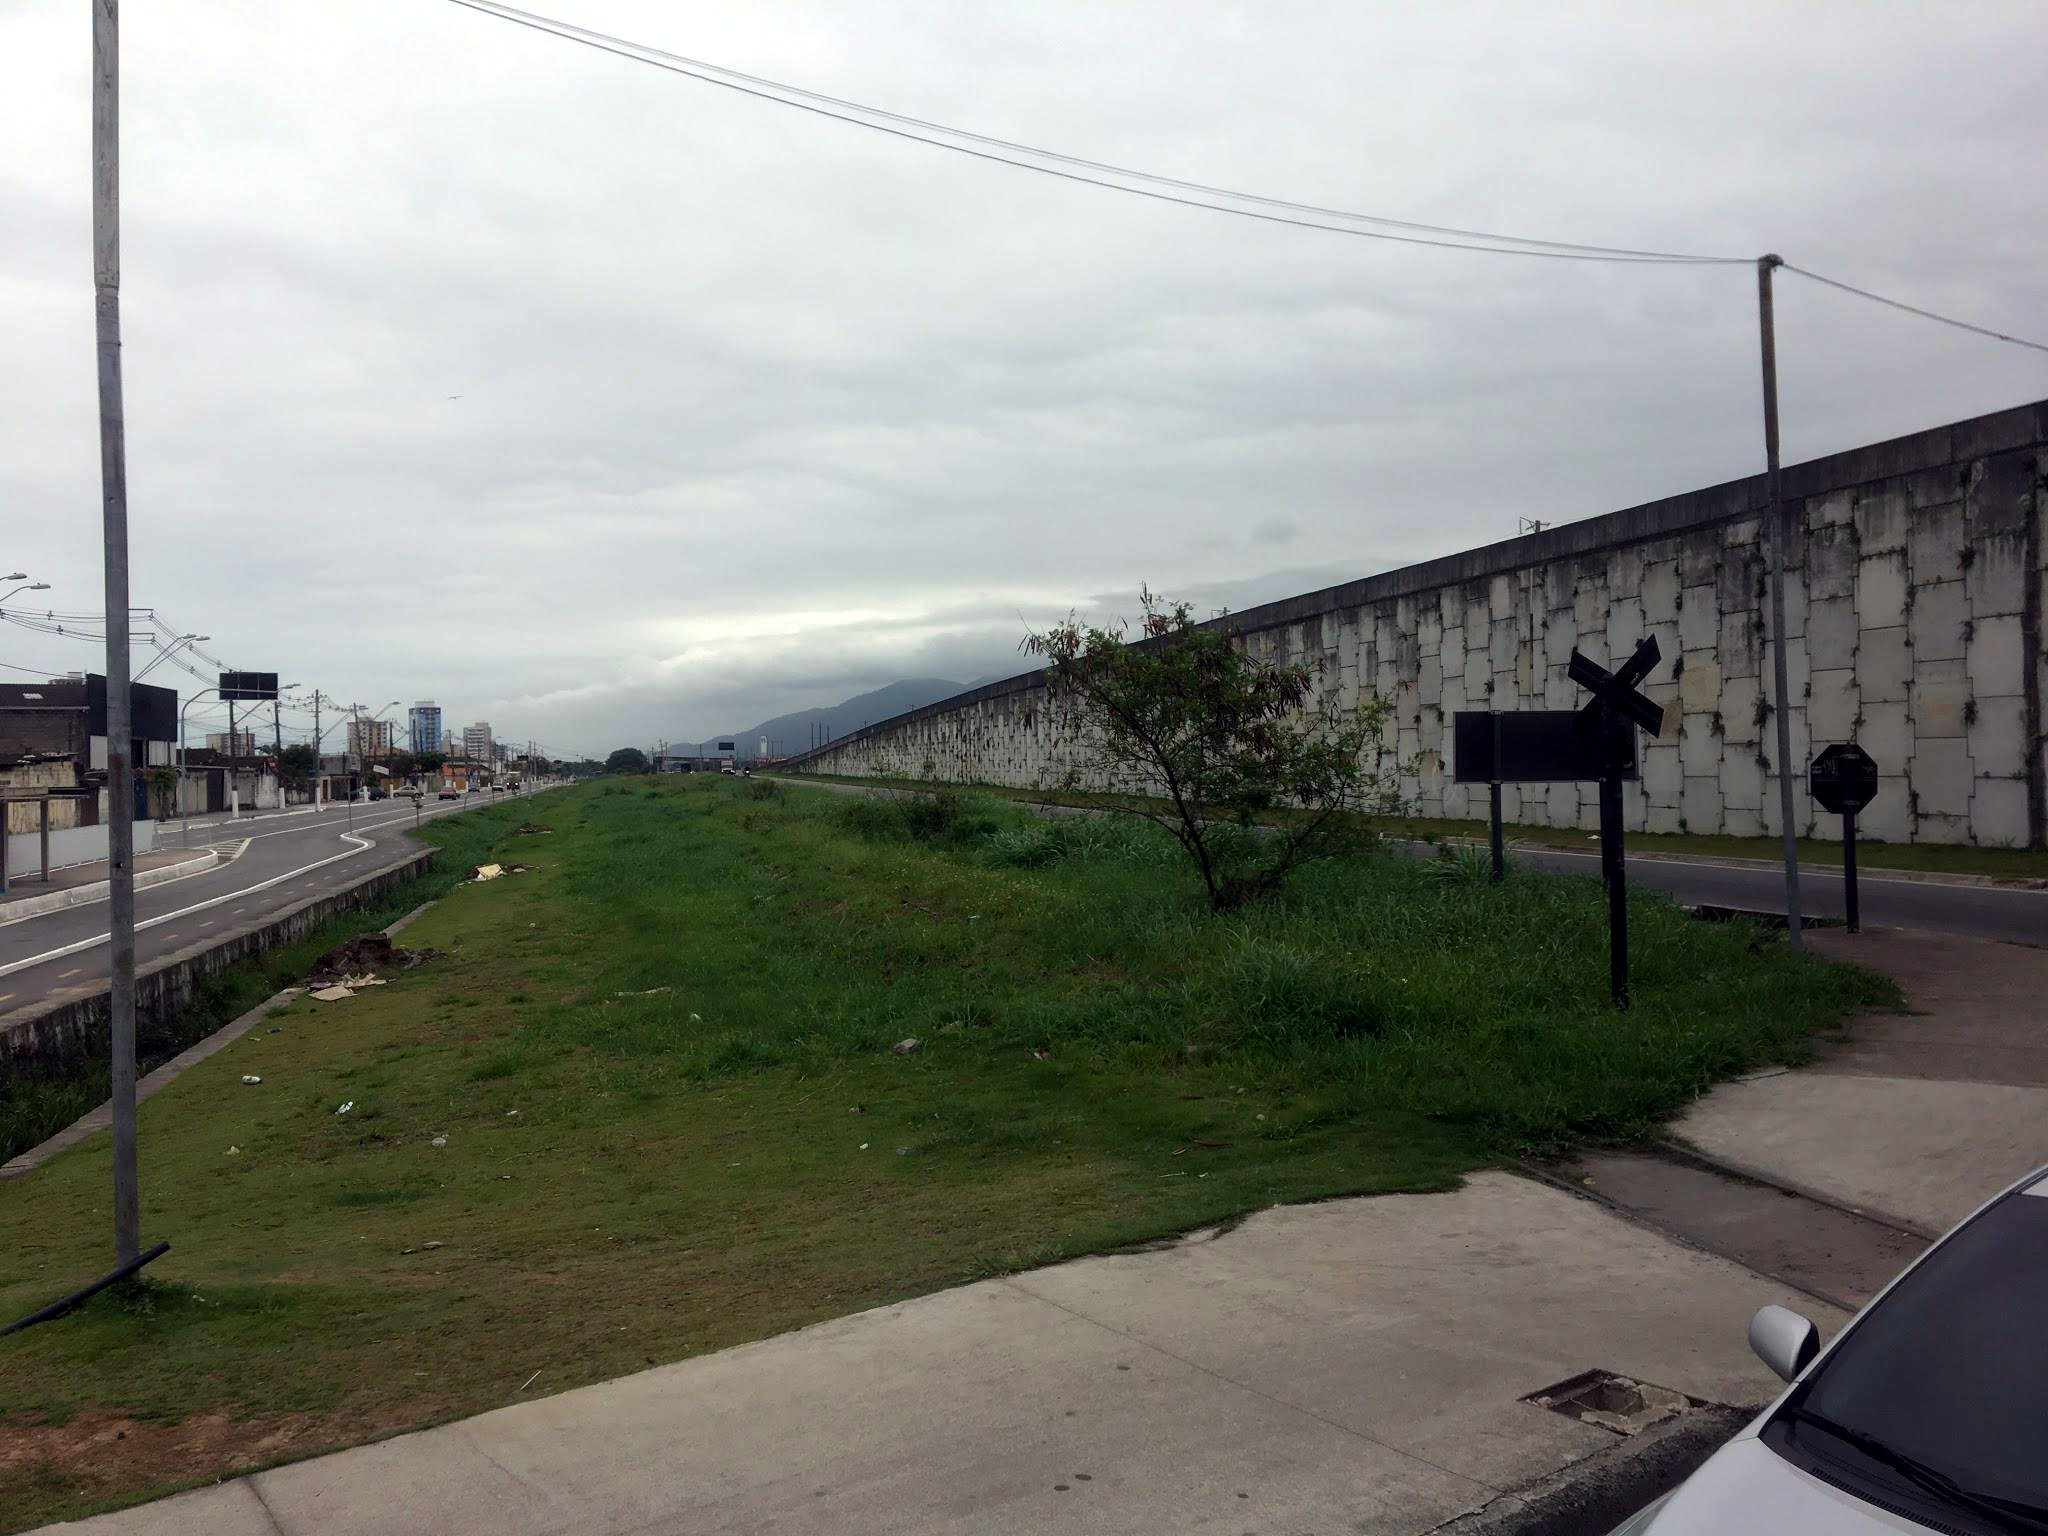
\includegraphics[width=1\textwidth]{img/foto_juquia.jpg}
		\label{foto_juquia}
		\legend{Elaboração própria}
	\end{figure}
	
	As antigas estações se encontram abandonadas, em ruínas ou se tornaram moradias, pois como aponta \citeonline[p.60]{Pires2011a}, ``quanto ao transporte de passageiros de longa distância, esse foi desativado no Brasil. As únicas exceções são as ferrovias controladas pela Vale que, por obrigação contratual, ainda realizam essa modalidade de transporte'', cabe salientar que no período estatal, \gls{rffsa} e \gls{fepasa} somadas contavam com 1.777 estações distribuídas pelo país, considerando o ano de 1995 \cite[p.61]{Pires2011a}, ainda, ``o estado atual dessas estações pode ser identificado como abandonada, demolida, utilizada como escritório operacional das concessionárias das ferrovias, recuperada como museus e centros culturais e até como moradia. Atualmente, grande parte dessas estações é considerada um obstáculo para a operação das ferrovias concessionadas e um problema para as prefeituras em virtude do uso inadequado das instalações'' \cite[p.61-62]{Pires2011a}.
	
	Sobre o ramal em aparente estado de abandono, \cite[p.321]{Zundt2006a}, recupera parte de seu caráter histórico ao apontar que ``a cultura da banana foi responsável, inclusive, pela extensão da malha ferroviária em direção ao sul da região e do estado, através do ramal Juquiá, da Estrada de Ferro Sorocabana''.

	\begin{landscape}
		\begin{figure}[p]
			\centering
			\caption{Ciclovias}
			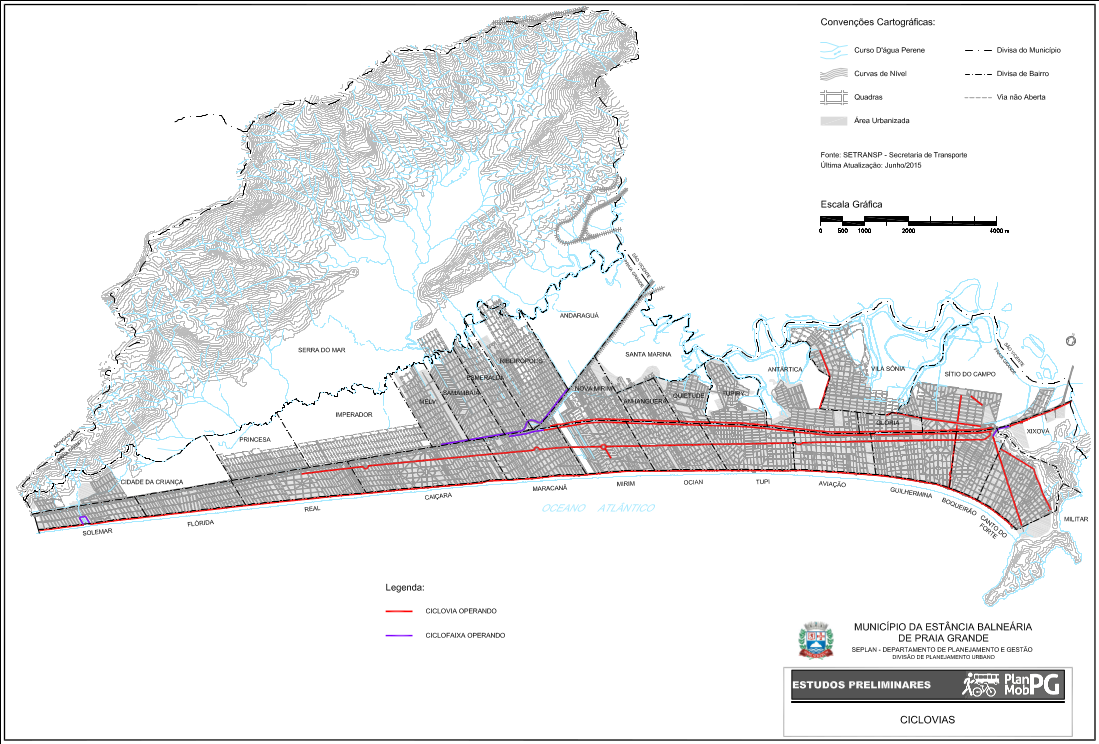
\includegraphics[width=21cm,height=21cm,keepaspectratio]{img/Ciclovias.png}
			\label{mapa_ciclovias}
			\legend{Fonte: \citeonline{secplan2016a}}
		\end{figure}
	\end{landscape}
		
	\subsection{Infraestrutura cicloviária}

	\begin{table}[!htb]
		\centering
		\caption{Ciclovias em operação no município de Praia Grande}
		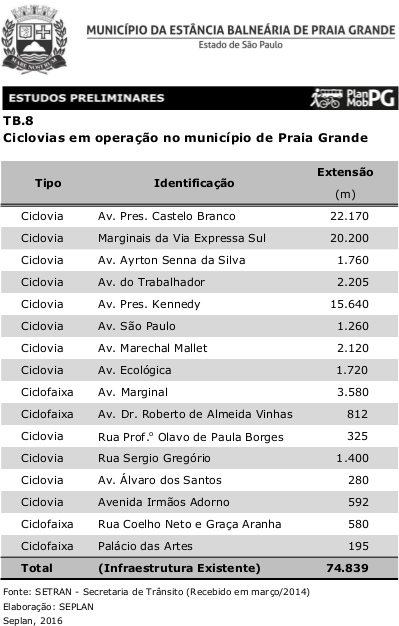
\includegraphics[width=0.4\textwidth]{img/TB_8_CICLOVIAS.png}
		\label{tab_ciclovias}
		\legend{Fonte: \citeonline{secplan2016a}}
	\end{table}
	
	A Figura \ref{tab_ciclovias} aponta e resume as principais informações de quilometragem e tipologia da cidade em relação à infraestrutura cicloviária, sendo oportuno destacar que a cidade oferta a infraestrutura nas principais vias de caráter estrutural, como a Av. Kennedy e a avenida beira-mar, algo que pode ser notado no mapa da Figura \ref{mapa_ciclovias}. Cabe salientar, no entanto, que não há intermodalidade e que a infraestrutura não está sendo complementada por para-ciclos e bicicletários.
	
	% = = = = = =
		
	\section{Meio-ambiente e saneamento integrado}
	% Parte da Noele
	
	\subsection{Bacia hidrográfica e áreas de drenagem}
	
	O município de Praia Grande faz parte da Bacia Hidrográfica da Baixada Santista, que abrange os municípios de Bertioga, Cubatão, Guarujá, Itanhaém, Mongaguá, Peruíbe, Praia Grande, Santos e São Vicente. \cite{ssrh2017a}

	O Plano Diretor de Drenagem e Manejo de Águas Pluviais de Praia Grande determina que Área de Drenagem é ``normalmente utilizada como parâmetro para o cálculo hidrológico e hidráulico das obras na bacia, sendo a área que contribui para o local de controle e que deve ser estimada através da determinação do divisor de águas''. \cite[p.142]{fcth2015a}

%	As áreas de drenagem do município estão concentradas na região da Serra do Mar, mais distante da praia, conforme a Figura \ref{mapa_dissecacao}.
%
%	\begin{figure}[h]
%		\centering
%		\caption{Mapa por \citeonline[p.312]{Souza2012a}: ``Carta de Dissecação Vertical do Município de Praia Grande (SP)''}
%		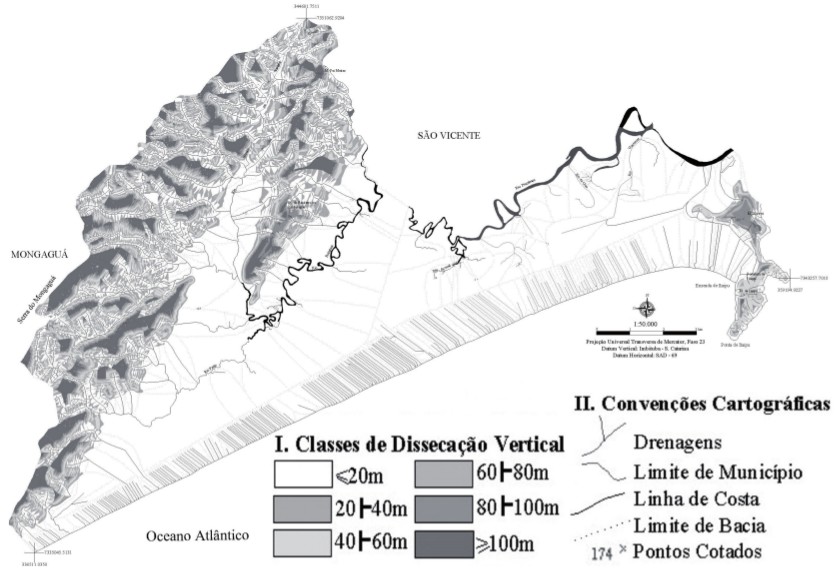
\includegraphics[width=1\textwidth]{img/classes_dissecacao_vertical.png}
%		\label{mapa_dissecacao}
%	\end{figure}

%	As áreas de drenagem naturais do município estão concentradas na região da Serra do Mar, mais distante da praia. Já as áreas de drenagem urbanas estão na região mais próxima das praias, direcionadas ao oceano ou aos rios Buturoca e Piaçabuçu \cite[p.191]{Cunha2015a}.

	As áreas de drenagem naturais do município estão concentrada na região da Serra do Mar, região mais distante da praia e com uma densidade populacional quase nula. Já as áreas de drenagem urbanas estão na região mais próxima das praias, onde se concentra a grande maioria da população do município, e são direcionadas ao oceano ou aos rios Buturoca e Piaçabuçu. Isso se deve a população predominantemente urbana no município, que está concentrada na faixa mais litorânea, deixando a região de serras mais deserta \cite[p.191]{Cunha2015a}.
	
	\begin{landscape}	
		\begin{figure}[h]
			\centering
			\caption{Bacia Hidrográfica da Baixada Santista}
			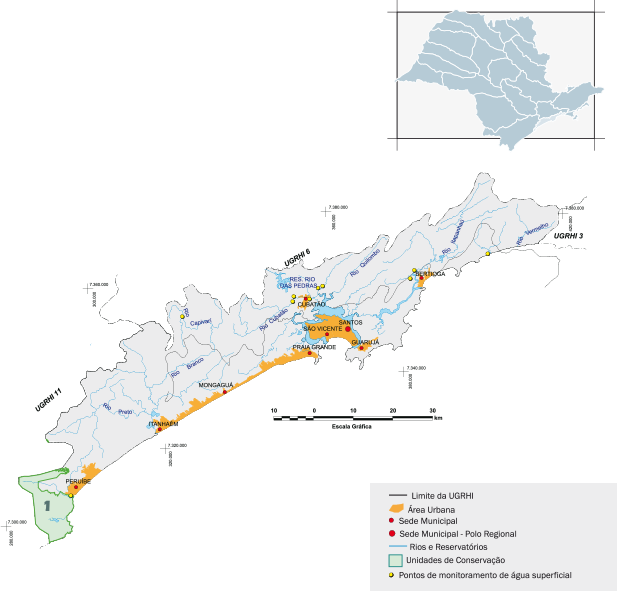
\includegraphics[width=15cm,height=15cm,keepaspectratio]{img/bacia_hidro.png}
			\label{mapa_bacia}
			\legend{Fonte: \citeonline{ssrh2017b}}
		\end{figure}
	\end{landscape}
	
	\begin{landscape}
		\begin{figure}[h]
			\centering
			\caption{Carta Geomorfológica do Município de Praia Grande (SP)}
			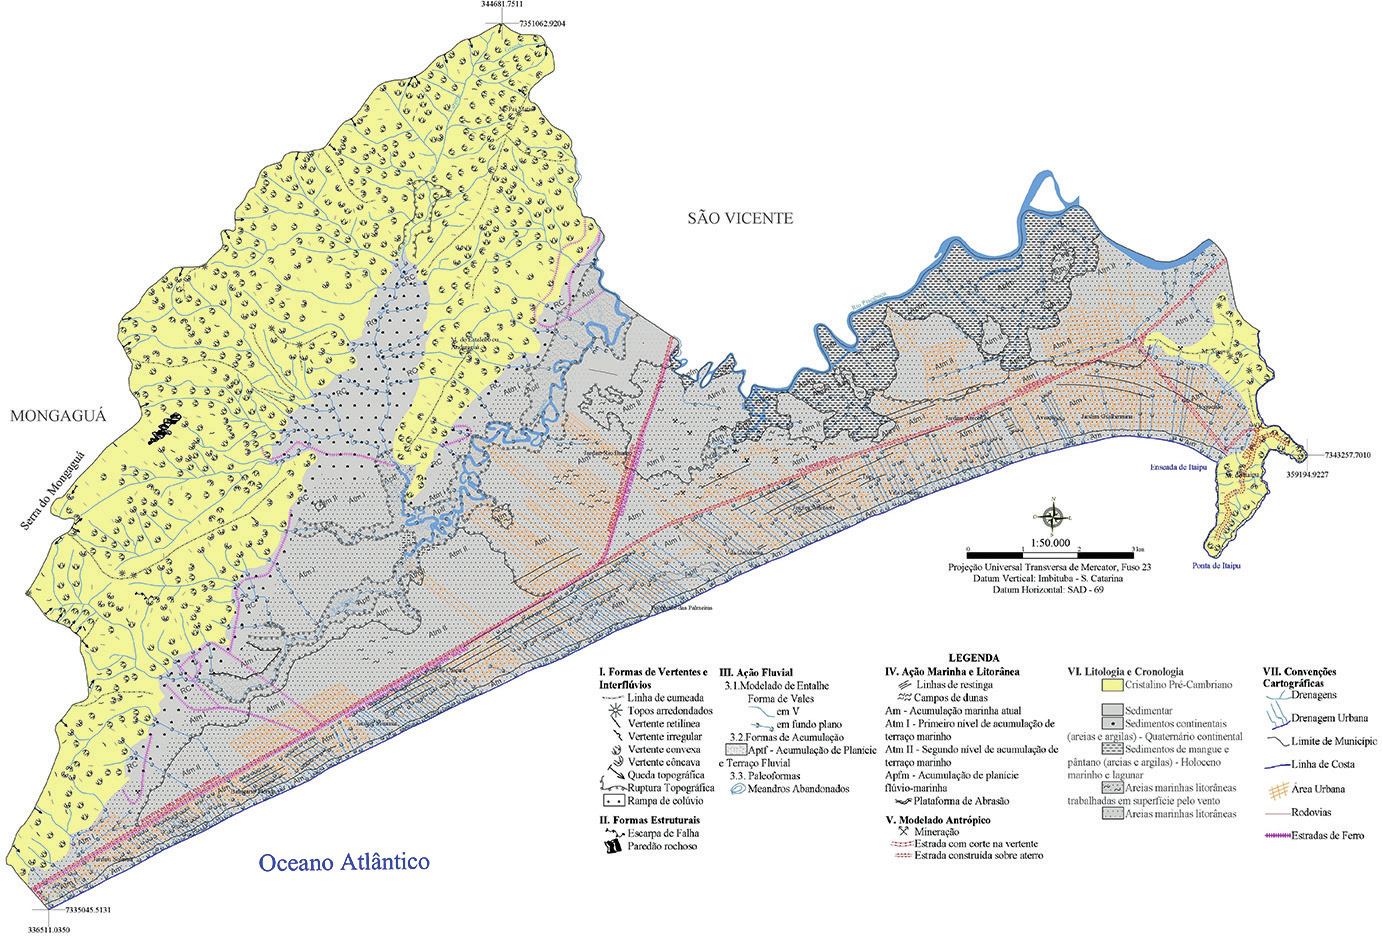
\includegraphics[width=21cm,height=21cm,keepaspectratio]{img/drenagem.png}
			\label{mapa_drenagem}
			\legend{Fonte: \citeonline[p.190]{Cunha2015a}}
		\end{figure}
	\end{landscape}
	
	\subsection{Áreas ambientalmente protegidas}
	
	O  município possui dois Parques Estaduais, o Parque Estadual da Serra do Mar e o Parque Estadual Xixová-Japuí. O primeiro, graças à legislação Decreto 10.251, de 30/08/77, 13.313, 06/03/79 e o segundo, a legislação Decreto 37.536, de 27/09/93. Ambos sob a responsabilidade do Instituto Florestal \cite{florestal2017a}.
	
	\subsection{Existência de APP urbana e situação}
	
	Segundo o Código Florestal (Lei n\textordmasculine 12.651, de 25 de maio de 2012), entende-se por Área de Preservação Permanente (\gls{app}): ``área protegida, coberta ou não por vegetação nativa, com a função ambiental de preservar os recursos hídricos, a paisagem, a estabilidade geológica e a biodiversidade, facilitar o fluxo gênico de fauna e flora, proteger o solo e assegurar o bem-estar das populações humanas'' \cite[Art. 3\textordmasculine, alínea II]{gf2012b}.
	
	No município de Praia Grande foram encontradas as seguintes \gls{app}:
		\begin{itemize}
			\item Margens de rios: o município possui alguns rios e córregos que foram analisados pelo Google Maps. Nenhum rio encontrado possui toda a \gls{app} preservada, alguns têm a maior parte preservada e outros apenas uma pequena parte. Como os exemplos a seguir:
			\begin{itemize}
				\item Rio Piaçabuçu, com cerca de 190 metros de largura (segundo medição feita no Google Maps), onde deve-se preservar 100 metros das margens. A maior parte das margens do rio está preservada, tendo uma pequena porção desmatada, conforme a Figura \ref{mapa_rio}.
				
					\begin{figure}[p]
						\centering
						\caption{Rio Piaçabuçu observado a partir do Google Maps}
						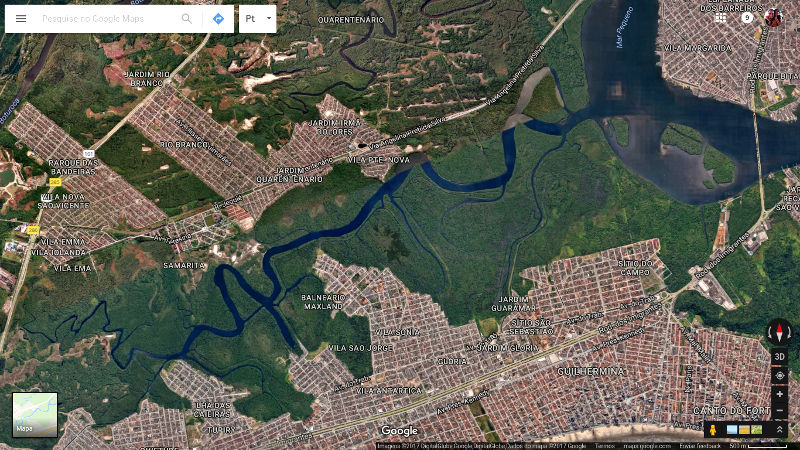
\includegraphics[width=0.8\textwidth]{img/maps_rio.png}
						\label{mapa_rio}
						\legend{Elaboração própria}
					\end{figure}
					
				\item Rio Itinga, com cerca de 5 metros de largura (segundo medição feita no Google Maps), onde deve-se preservar 30 metros das margens. Porém apenas cerca de 5 metros das margens está preservado no trecho urbano, conforme a Figura \ref{mapa_rio2}.
							
					\begin{figure}[p]
						\centering
						\caption{Rio Itinga observado a partir do Google Maps}
						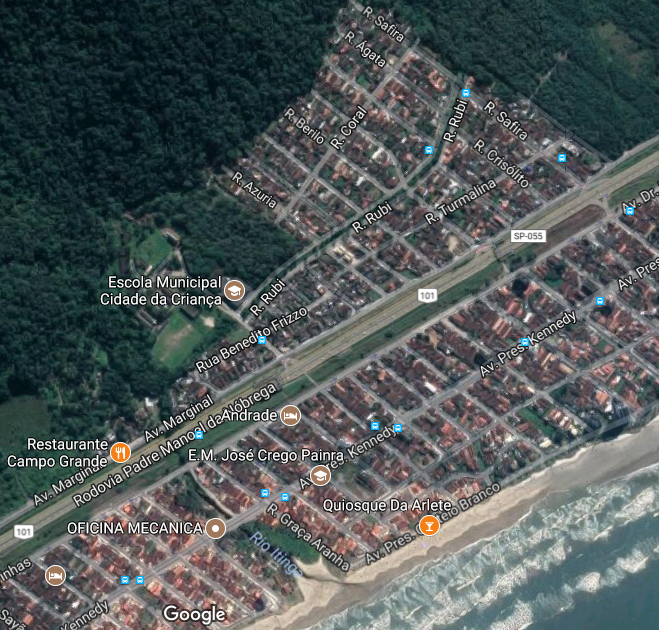
\includegraphics[width=0.8\textwidth]{img/maps_rio2.png}
						\label{mapa_rio2}
						\legend{Elaboração própria}
					\end{figure}

			\end{itemize}
			\item Nascentes: não há uma lista das nascentes presentes no município, porém a prefeitura tem um projeto para mapeamento e preservação das nascentes chamado ``Nascente Municipal Modelo'' (SMAPG) \cite{pmpg2017c}
			\item Encostas ou topos de Morro: O município possui declividades acima de 45 graus apenas na região serrana, que está preservada com mata.
			\item Restinga: O município, por ser litorâneo, possuía uma grande quantidade de restinga. Porém com a urbanização, perdeu a grande maior parte dessa vegetação \cite[p.191]{Cunha2015a}.
			\item Manguezal: O município possui área de mangue que está sendo preservada. Mas existem relatos de lixo espalhado na região de mangue \cite{Sellis2014a}.
		\end{itemize}
	
	\subsection{Áreas de risco ou com restrição à ocupação}
	
	Em 2014 o município de Praia Grande passou a integrar o mapeamento de áreas de risco da Defesa Civil. Como resultado, obteve-se a Carta Municipal de Suscetibilidade do município, apresentada nas Figuras \ref{mapa_susce}, \ref{quadroA_susce} e \ref{quadroB_susce}.
	
	\begin{figure}[h!]
		\centering
		\caption{Mapa de Suscetibilidade do Município de Praia Grande}
		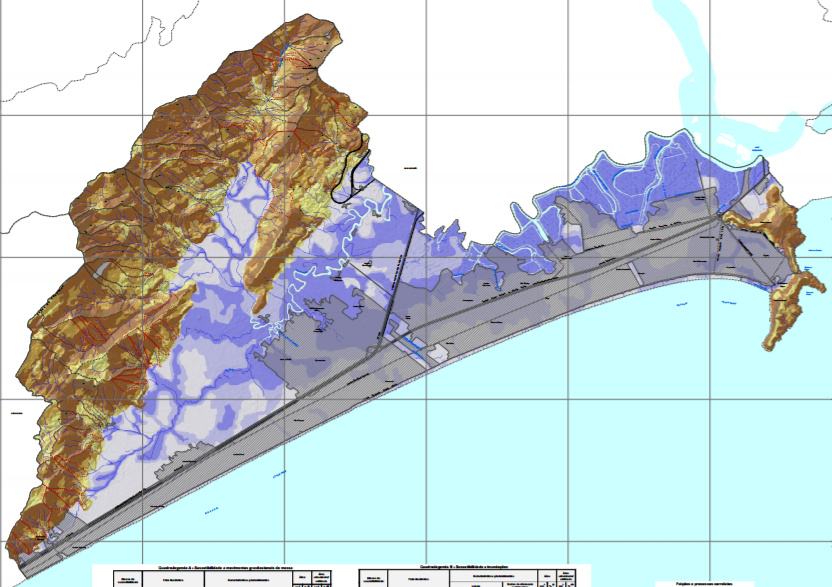
\includegraphics[width=1\textwidth]{img/mapa_suscetibilidade.png}
		\label{mapa_susce}
		\legend{Fonte: \citeonline{IPT2015a}}
	\end{figure}

	\begin{landscape}
		\begin{minipage}[b]{0.5\linewidth}
			\captionof{figure}{Suscetibilidade a movimentos gravitacionais de massa}
			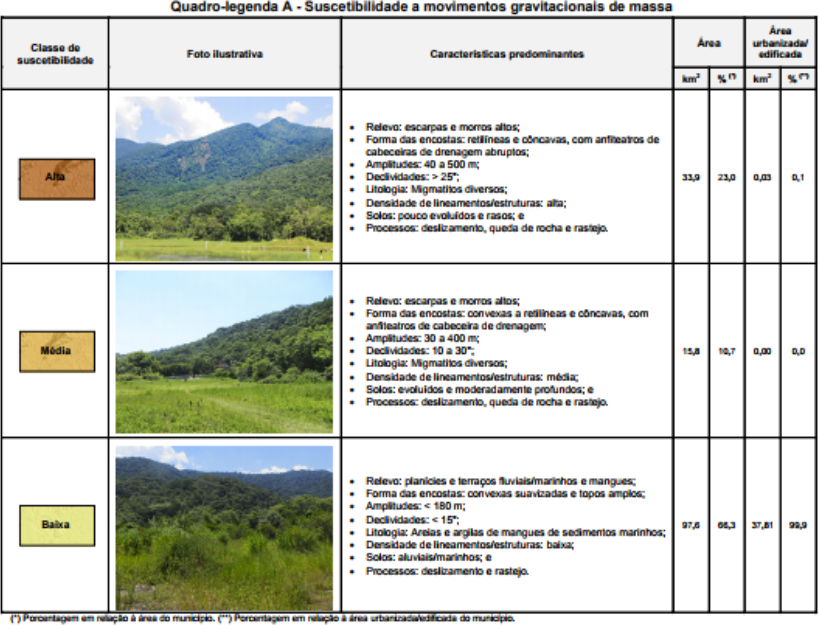
\includegraphics[width=12cm,height=12cm,keepaspectratio]{img/quadroA_suscetibilidade.png}
			\label{quadroA_susce}
			\legend{Fonte: \citeonline{IPT2015a}}
		\end{minipage}
		\begin{minipage}[b]{0.5\linewidth}
			\captionof{figure}{Suscetibilidade a inundações}
			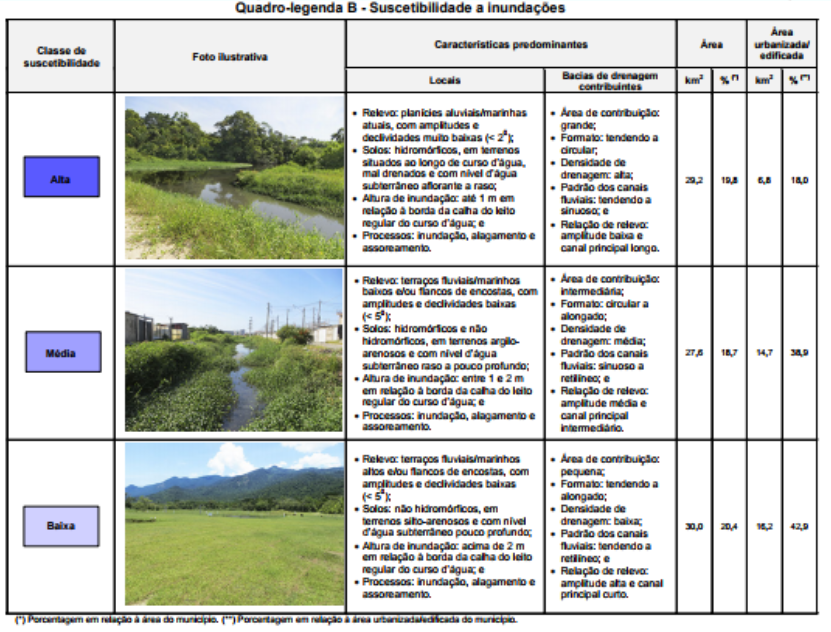
\includegraphics[width=11cm,height=11cm,keepaspectratio]{img/quadroB_suscetibilidade.png}
			\label{quadroB_susce}
			\legend{Fonte: \citeonline{IPT2015a}}
		\end{minipage}
	\end{landscape}

	\subsection{Coleta e destinação de esgoto}
	
	No município há 4.254 (4,04\% do total) ligações factíveis (quando a rede está disponível, mas a ligação não é feita), ou seja, que não destinam o esgoto corretamente para o tratamento realizado pela \gls{sabesp} (Companhia de Saneamento Básico do Estado de São Paulo) \cite{Rossi2017a}.
	
	Segundo a \gls{sabesp} 100\% do esgoto coletado em Praia Grande é tratado para a retirada de material sólido e flutuante através de 7 peneiras rotativas. Após o tratamento o esgoto é lançado ao mar por meio do sistema de emissário submarino. Os resíduos são diluídos e afastados do litoral pelas correntes marítimas a cerca de 3 300 metros da costa e a uma profundidade de 16 metros \cite{Carvalho2014a}.
	
	O esgoto da Praia Grande é ``processado em três estações de pré-condicionamento \textemdash Forte, Tupi e EPC 3 \textemdash com capacidade total de 3.181,7 litros por segundo'' \cite{Sabesp2017a}.
	
	\subsection{Volume de produção de resíduos sólidos; coleta e disposição de resíduos e soluções encontradas pelo município}
	
	No ano de 2012 o município produziu cerca de 898,2 t/dia de resíduos sólidos, conforme Tabela \ref{quadro_prod_resid_urbanos}. Quanto à coleta dos resíduos, a prefeitura estabelece as seguintes responsabilidades (Tabela \ref{quadro_responsa_resid_urbanos})\footnote{Sendo Classe I (Resíduos Perigosos), Classe II (Resíduos não Perigosos, não inertes) e Classe III (Resíduos não Perigosos, inertes.)}.
	
	\begin{table}[!htb]
		\centering
		\caption{Resumo da produção de resíduos urbanos}
		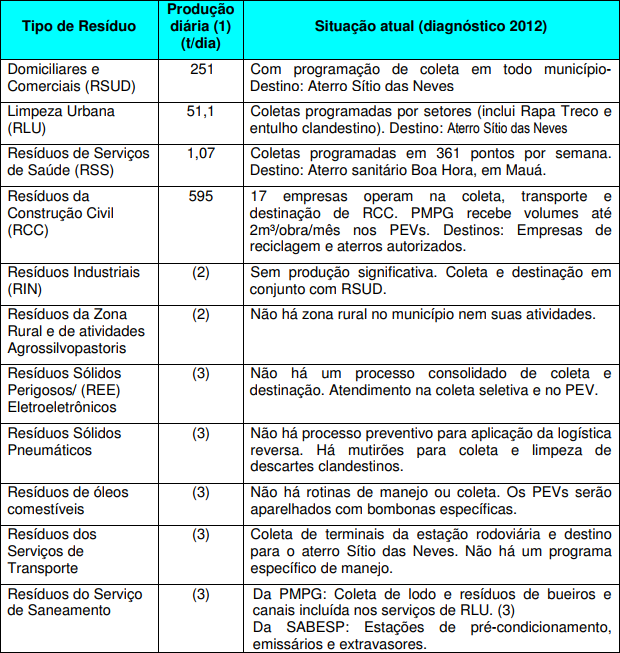
\includegraphics[width=1\textwidth]{img/prod_resid_urbanos.png}
		\label{quadro_prod_resid_urbanos}
		\legend{Fonte: \citeonline[p.118]{pmpg2014a}}
	\end{table}
	
	\begin{table}[!htb]
		\centering
		\caption{Classificação da produção de resíduos urbanos}
		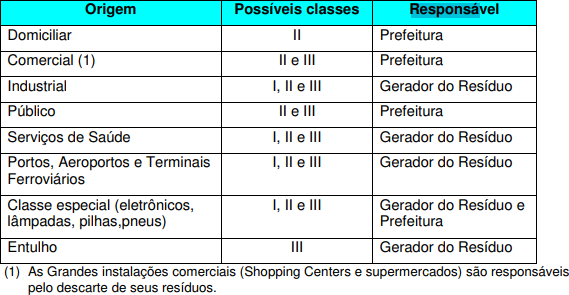
\includegraphics[width=1\textwidth]{img/responsa_resid_urbanos.png}
		\label{quadro_responsa_resid_urbanos}
		\legend{Fonte: \citeonline[p.58]{pmpg2014a}}
	\end{table}
	
	O município possuía um lixão, que foi desativado. Atualmente seus resíduos municipais são transportados para o aterro Sítio das Neves, no município de Santos. O serviço de transporte é devidamente licenciado pelo CADRI \textemdash Certificado de Movimentação de Resíduos de Interesse Ambiental. Os resíduos de serviços de saúde (RSS) são descartados nas instalações de incineração da Silcon Ambiental, no Município de Mauá \cite[p.113]{pmpg2014a}.
		
	\subsection{Serviço de abastecimento de água}

	Os serviços de água e esgoto no município de Praia Grande estão sob gestão da \gls{sabesp} desde dezembro de 1975 \cite{Sabesp2017a}, outrossim ``a cidade recebe água dos sistemas Cubatão, Pilões, Melvi e Mambu-Branco que pertencem ao Sistema Integrado da Baixada Santista. O Sistema também abastece os municípios de Bertioga, Cubatão, Itanhaém, Guarujá, Mongaguá, Santos e São Vicente, com capacidade total de 1.600 litros por segundo'' \cite{Sabesp2017a}.
	
	\begin{center}
		\begin{longtable}{l l}
			\caption{Taxa Geométrica de Crescimento Anual da População (em \% a.a.)} \label{tab_tgca}\\
			\hline
			\textbf{Aspecto} & \textbf{Valor} \\
			\hline
			\endfirsthead
			\multicolumn{2}{c}%
			{\tablename\ \thetable\ -- \textit{Continuado da página anterior}} \\
			\hline
			\textbf{Aspecto} & \textbf{Valor} \\
			\hline
			\endhead
			\hline \multicolumn{2}{r}{\textit{Continua na próxima página}} \\
			\endfoot
			\hline
			\endlastfoot
			Ligações de água: & 103,943 \\
			Economias de água: & 221,859 \\
			Extensão de redes de água: & 941.15 quilômetros \\
			Estações de tratamento de água: & - \\
			Poços: & - \\
			Reservatórios: & 3 \\
			Capacidade de reservação: & 25,000 milhões de litros \\
		\end{longtable}
		\legend{Elaboração própria. Fonte: \citeonline{Sabesp2017a}}
	\end{center}	
	
	\subsection{Sistema de água pluviais e existência de áreas sujeitas a inundação}
	
	A prefeitura de Praia Grande possui um Plano Diretor de Drenagem e Manejo de Águas Pluviais (\gls{pddmap}), que delimita metas e ações para melhorar a drenagem do município, eliminar o despejo ilegal de esgoto no sistema pluvial e assim, melhorar a qualidade das águas das praias e a paisagem local.
	
	O Plano visa  dois objetivos básicos: controle do aumento da vazão máxima e melhoria das condições ambientais. As medidas de controle do escoamento podem ser classificadas, de acordo com sua ação na bacia hidrográfica, em:
	
	\begin{citacao}
		\begin{itemize}
			\item ``distribuída ou na fonte: é o tipo de controle que atua sobre o lote, praças e passeios na microdrenagem, é o controle que age sobre o hidrograma resultante de um parcelamento ou mesmo de mais de um parcelamento, para áreas inferiores a 2 km$^{2}$'';
			\item na macrodrenagem: é o controle sobre áreas acima de 2 km$^{2}$ ou dos principais rios urbanos.'' \cite[p.7]{fcth2015a}
		\end{itemize}
	\end{citacao}

	Com isso, espera-se reduzir os alagamentos, que como vimos no Mapa de Suscetibilidade do Município de Praia Grande (Figura \ref{mapa_susce}), abrange boa parte da zona urbana do município.
	
	A precipitação média anual do município é de menos de 2000 mm na maior parte do território, porém tem região com mais de 2100 mm, conforme mapa (Figura \ref{mapa_precipitacao}).
	
	\begin{figure}[htb]
		\centering
		\caption{Precipitações médias anuais e mensais}
		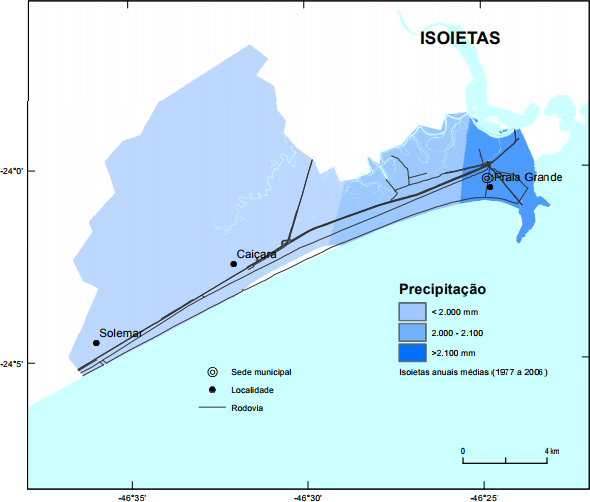
\includegraphics[width=1\textwidth]{img/mapa_precipitacao.png}
		\label{mapa_precipitacao}
		\legend{Fonte: \citeonline{IPT2015a}}
	\end{figure}	
	
	A precipitação no município é maior no verão e reduz bastante no inverno, como observado na região sudeste como um todo. Conforme Figura \ref{graf_precipitacao}:
	
	\begin{figure}[H]
		\centering
		\caption{Precipitação anual}
		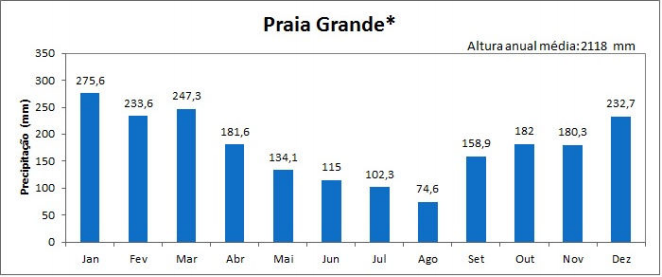
\includegraphics[width=1\textwidth]{img/precipitacao.png}
		\label{graf_precipitacao}
		\legend{Fonte: \citeonline{IPT2015a}}
	\end{figure}	
	
	\subsection{Poluição/contaminação do ar/água/solo}
	
%	Segundo a \gls{cetesb} , todas as praias do município estão próprias para banho atualmente. O que indica que o nível de poluição das águas das praias está dentro do aceitável para o contato com seres humanos.
	
	A \gls{cetesb}, mostra a qualidade das água das praias no estado de São Paulo diariamente. Nós monitoramos a qualidade das águas em Praia grande uma vez por semana durante um mês e como resultado obtivemos que todas as praias do município estavam próprias para banho antes do feriado de 02 de novembro, o que indica que o nível de poluição das águas das praias estava dentro do aceitável para o contato com seres humanos. Porém, após o feriado, três praias (Vila Tupi, Boqueirão e Maracanã) se mostraram impróprias para banho, conforme Figura \ref{mapa_qualidade_agua}. Provavelmente isso se deve ao aumento populacional que o município apresenta durante feriados prolongados, por conta das moradias de veraneio. O que aumenta a produção e despejo de poluentes nas águas.
	
	\begin{figure}[!htb]
		\centering
		\caption{Qualidade das águas das praias no município de Praia Grande}
		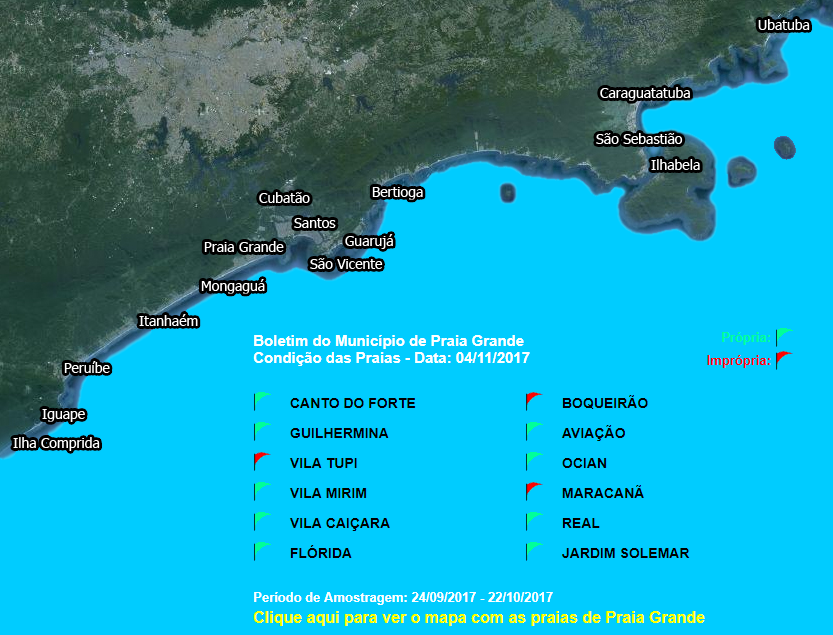
\includegraphics[width=1\textwidth]{img/mapa_qualidade_agua.png}
		\label{mapa_qualidade_agua}
		\legend{Fonte: \citeonline{cetesb2017b}}
	\end{figure}
	
	A \gls{cetesb} não possui estação de medição dos níveis de poluentes no município, porém, os municípios próximos apresentaram bons índices de poluição do ar no período observado, conforme Tabela \ref{tab_qualidade_ar} e Tabela \ref{tab_qualidade_ar2}.
	
	\begin{table}[!htb]
		\centering
		\caption{Qualidade do Ar em 09/10/2017, 20h}
		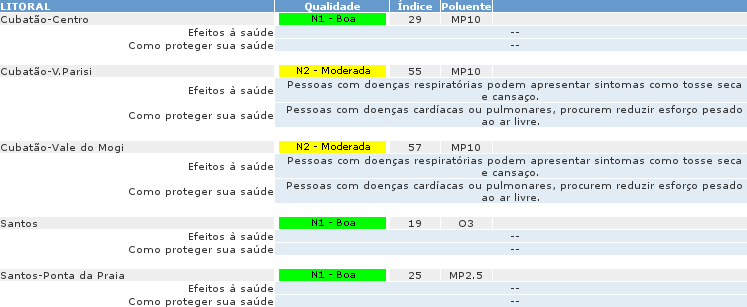
\includegraphics[width=1\textwidth]{img/tab_qualidade_ar.png}
		\label{tab_qualidade_ar}
		\legend{Fonte: \citeonline{cetesb2017a}}
	\end{table}
	
	\begin{table}[!htb]
		\centering
		\caption{Qualidade do Ar em 06/11/2017, 7h}
		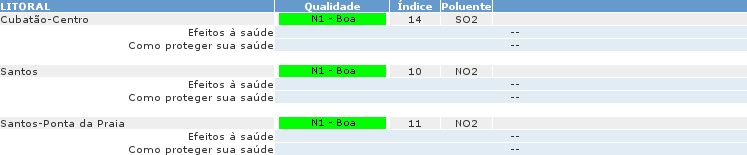
\includegraphics[width=1\textwidth]{img/tab_qualidade_ar2.png}
		\label{tab_qualidade_ar2}
		\legend{Fonte: \citeonline{cetesb2017a}}
	\end{table}
	
	\subsection{Cemitérios}
	
	O único cemitério encontrado no município é o Cemitério Morada da Grande Planície, que é municipal. Não foram encontrados dados a respeito da drenagem realizada no local e nada que indique que há um trabalho de prevenção a contaminação do solo. O que nos leva a pensar que nada é feito para evitar que o solo e lençol freático sejam contaminados com patógenos e chorume presentes no local.
		
%
%===============================================================================
%

	\chapter{Ação Governamental}
	
	\section{Do Plano Diretor}
	
	O Plano Diretor de Praia Grande, embora extenso, é bastante segmentado no que se refere aos instrumentos de aplicação. Dispõe de pelo menos 16 Planos Setoriais, Planos Temáticos, Urbanísticos, de Desenvolvimento Econômico e Social, além do Plano Plurianual de Investimentos. 
	
	A amplitude de atribuições pretendidas pelo \gls{pde} somada à setorização da política do município reflete certa desconexão com o território, fazendo com que a integração das políticas territoriais não sejam tratadas no Plano como uma prioridade. Questões inerentemente espaciais, tais como habitação, saneamento e mobilidade, quando tratadas isoladamente, ressoam negativamente na aplicação de outras políticas \textemdash como educação, saúde e segurança. 
	
	Sua estrutura organizacional reflete tal segmentação, contando com 20 secretarias. São elas:
	
	\begin{itemize}
		\item Gabinete do Prefeito
		\item Secretaria de Urbanismo
		\item Procuradoria Geral do Município
		\item Secretaria de Administração
		\item Secretaria de Segurança
		\item Secretaria de Transporte
		\item Secretaria de Cultura e Turismo
		\item Secretaria de Desenvolvimento Econômico, Ciência, Tecnologia e Trabalho
		\item Secretaria da Educação
		\item Secretaria de Esporte e Lazer
		\item Secretaria de Finanças
		\item Secretaria de Governo
		\item Secretaria de Habitação
		\item Secretaria de Meio Ambiente
		\item Secretaria de Obras
		\item Secretaria de Planejamento
		\item Secretaria de Promoção Social
		\item Secretaria de Saúde
		\item Secretaria de Serviços Urbanos 
		\item Secretaria de Trânsito 
	\end{itemize}
	
	Algumas leis foram destacadas devido a sua importância no ordenamento da cidade, como mostra o quadro a seguir (contém hiperlinks):
	
	\begin{center}
		\begin{longtable}{|p{120pt} | p{120pt} | p{50pt} | p{100pt}|}
			\caption{Quadro-síntese: legislação de especial relevância} \label{tab_especial_ordenamento}\\
			\hline
			\textbf{Assunto} & \textbf{Norma} & \textbf{Vigência} & \textbf{Endereço} \\
			\hline
			\endfirsthead
			\multicolumn{4}{c}%
			{\tablename\ \thetable\ -- \textit{Continuado da página anterior}} \\
			\hline
			\textbf{Assunto} & \textbf{Norma} & \textbf{Vigência} & \textbf{Endereço} \\
			\hline
			\endhead
			\hline \multicolumn{4}{r}{\textit{Continua na próxima página}} \\
			\endfoot
			\hline
			\endlastfoot
			Plano Diretor & Lei Complementar N\textordmasculine 727 DE 16 DE DEZEMBRO DE 2016 & 2017/2026 & \url{https://goo.gl/AofUfP} \\ \hline
			Ordenamento do uso, ocupação e parcelamento do solo & Lei Complementar N\textordmasculine 615 DE 19 DE DEZEMBRO DE 2011 & - & \url{https://goo.gl/JcsQVY} \\ \hline
			Plano Municipal de Habitação de Interesse Social & 	Lei N\textordmasculine 1547 DE 14 DE ABRIL DE 2011 & - & \url{https://goo.gl/C69Ufa} \\ \hline
			Plano Plurianual & Lei N\textordmasculine 1688 DE 25 DE OUTUBRO DE 2013 & 2015/2025 & \url{https://goo.gl/RnmFFv} \\ \hline
			Política Municipal de Saneamento Básico & Lei N\textordmasculine 1697 DE 2 DE DEZEMBRO DE 2013 & 4 anos & \url{https://goo.gl/7tqNfa} \\ \hline
			Plano Diretor de Drenagem e Manejo de Águas Pluviais & Lei N\textordmasculine 1823 DE 16 DE DEZEMBRO DE 2016 & 20 anos & \url{https://goo.gl/YZXyYF} \\ \hline
			Plano Municipal de Gestão Integrada de Resíduos Sólidos & LEI N\textordmasculine 12.305, DE 2 DE AGOSTO DE 2010 & - & \url{https://goo.gl/uZi4MG} \\ \hline
		\end{longtable}
		\legend{Elaboração própria}
	\end{center}	
	
	Outros planos importantíssimos como Plano Diretor de Turismo (como disposto em Lei Complementar N\textordmasculine 1.261, de 29 de abril de 2015) e Plano de Mobilidade Urbana estão em fase de elaboração. 

	% = = = = = =
	
	\section{Projetos especiais}
	
	Algumas secretarias desenvolvem projetos que se destacam entre os serviços que normalmente são realizados pelos municípios. A seguir, será feita uma breve descrição de alguns desses projetos.
	
	\subsection{Secretaria de Serviços Urbanos}
	
	Responsável pela limpeza urbana, manutenção da orla, drenagem, iluminação pública e serviços gerais. Possui projetos como o Rapa Treco e o Eco Ponto.
	
	O programa Rapa Treco realiza diariamente de objetos como móveis, eletrodomésticos, colchões, sofás e utensílios domésticos descartados incorretamente em vias e terrenos públicos \cite{deMarco2015a}. Seu cronograma de atuação está disponível através do sítio eletrônico da prefeitura de Praia Grande.
	
	O programa Eco Ponto foi criado para prevenir o descarte de materiais considerados sem utilização em locais inapropriados. Hoje o programa, criado em janeiro de 2012, conta com pontos localizados em 11 bairros diferentes do município. \cite{pmpg2017d}
	
	\subsection{Secretaria de Meio Ambiente}
	
	No geral, além de promover o desenvolvimento urbano, econômico e socialmente sustentável, a Secretaria de Meio Ambiente também tem como atribuição prestar assistência técnica às demais secretarias no campo ambiental. Entre os projetos que podem se destacar estão os programas Esgoto Certo, Gestão das Águas e Onda Limpa.
	
	Esgoto Certo é um programa que tem como foco detectar ligações de esgoto irregulares, intimando os proprietários a fazerem a regularização. Conta com um número telefônico para recebimento de denúncias. \cite{pmpg2017e}
	
	Gestão das Águas é voltado à identificação das nascentes no território do município \cite{pmpg2017f}.
	
	O programa Onda Limpa é um convênio do município com a \gls{sabesp} que visa coletar e tratar 100\% do esgoto do município. Conta com um plano de expansão da infraestrutura orçado em R\$ 120 milhões \cite{pmpg2017g}.
	
	\subsection{Secretaria de Transportes}
	
	``Responsável por organizar, administrar e fiscalizar os serviços de transporte coletivo municipal de passageiros, de táxi e de escolares'' \cite{pmpg2017h}.
	
	Há um corredor de ônibus sendo projetado pelo município entre os bairros Mirim e Solemar com recursos advindos do \gls{pac} \cite{pmpg2017i}.

	\subsection{Secretaria de Habitação}
	
	Dentro da Secretaria Municipal de Habitação o programa Dono do Lote se destaca por conceder o título de Direito Real de Uso para cerca de 15\% da população fixa do município. Programa está dentro do âmbito da lei de Regularização Fundiária (lei municipal n\textordmasculine 671/13) \cite{pmpg2017j}.
	
	\subsection{Secretaria de Urbanismo}
	
	Ainda em processo de negociação, encontra-se o programa Gestão da Orla que se refere a um compromisso do município com a constante melhoria dos espaços litorâneos, via um acordo firmado entre o município e a Secretaria de Patrimônio da União. O programa ainda encontra-se em fase de negociação, com audiência pública marcada para o dia 30 de outubro de 2017 \cite{pmpg2017k}.

%
%===============================================================================
%

	\chapter{Síntese}
	
	A parcela urbana de Praia Grande pode ser dividida em duas diferentes cidades, antagônicas em suas características, divididas pelo histórico de ocupação e continuadas pelo efeito barreira da rodovia e reafirmação da vocação de turismo de veraneio que rege o município, de forma que boa parte dos obstáculos relativos a habitação, saneamento e mobilidade decorrem dessa lógica.
	
	A falta de transparência e dificuldade de dimensionamento dos dados de habitação configuram um  impasse à solução do déficit habitacional, considerando-o quantitativa e qualitativamente. Visto que boa parte dos assentamentos precários estão localizados próximos à áreas de proteção ambiental, o adensamento não planejado ou desordenado impactaria negativamente nessas áreas. Para que seja possível qualificar o adensamento populacional, as \gls{zeis} e demais mecanismos, como o \gls{plhis} e a \gls{luops} demandam, além de regulamentação mais rígida na legislação,  vontade política.
	
	O outro lado da rodovia configura, por sua vez, outro tipo de cidade, de turismo sazonal intenso e infra-estrutura adequada. Todavia, apresenta também grandes vazios urbanos, de modo que áreas que possuem grande oferta de equipamentos públicos são subaproveitadas, servindo à especulação imobiliária e intensificando a segregação socioespacial, na contramão da aplicação da função social da cidade de função social  da propriedade urbana.
	
	No que se refere ao saneamento básico, as dificuldades são regionais, posto que grande parte dos municípios carece de coleta de esgoto e tratamento adequados. Devido o desequilíbrio entre alta e baixa temporada, essa situação é agravada em Praia Grande. Em períodos sazonais o abastecimento de água é insuficiente principalmente nos bairros que concentram população residente. A intensificação na contaminação por resíduos não coletados ou tratados de forma inadequada pode ressoar nos índices de balneabilidade, causando impactos negativos no turismo.
	
	A cidade apresenta um sistema de transporte coletivo com menos de 20 linhas municipais, 2 terminais de ônibus e que, dependendo da articulação metropolitana sob responsabilidade do Governo do Estado de São Paulo, poderá adquirir um caráter mais estruturante.
    
	\begin{landscape}
		\begin{figure}[h]
			\centering
			\caption{Mapa Síntese do Diagnóstico de Praia Grande}
			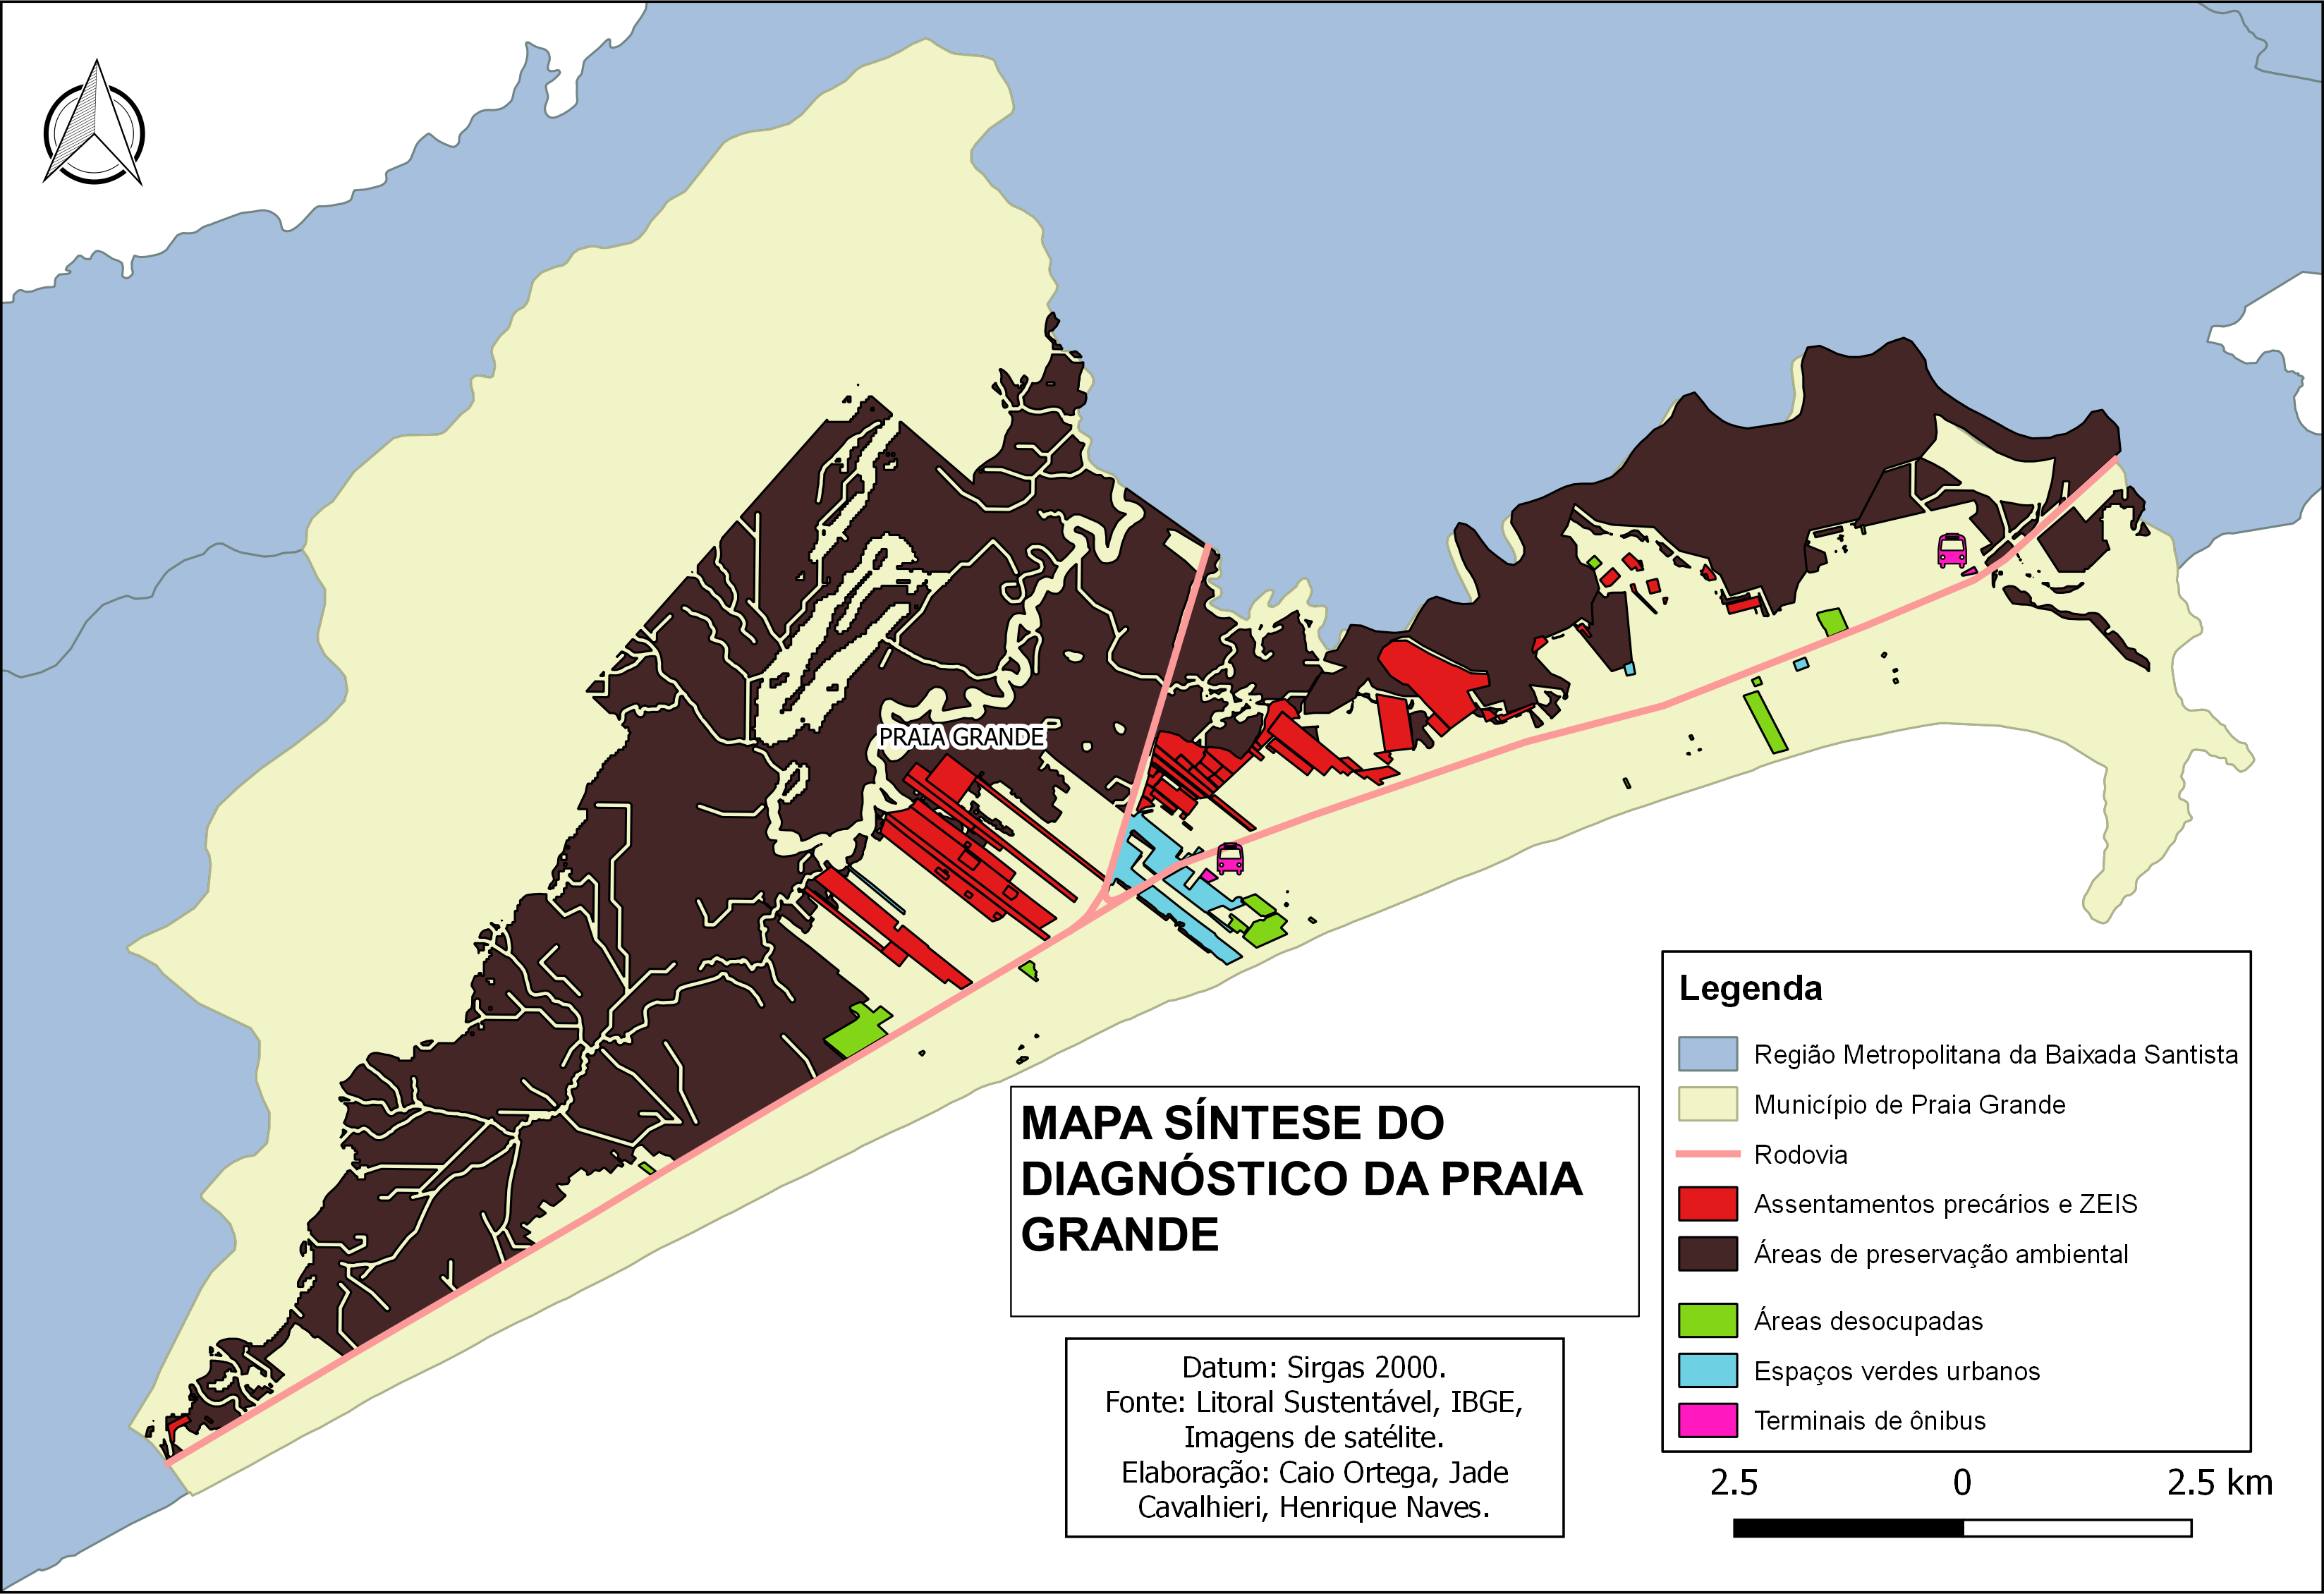
\includegraphics[width=22cm,height=22cm,keepaspectratio]{img/mapa_sintese_praia_grande_final.png}
			\label{mapa_sintese_pg}
			\legend{Elaboração própria}
		\end{figure}
	\end{landscape}

%
%===============================================================================
%

	\chapter{Diretrizes}
	% Consulta do quadro-síntese:
	% https://docs.google.com/spreadsheets/d/1cvtblNHAzuRlXYAJWQqDFzxBNsPGyaflwYrQkmsySvk/edit#gid=0
		
	Para a elaboração das diretrizes, a Carta de Delimitação de Zonas Especiais de Interesse Social anexa ao Plano Diretor  e a Carta de Uso e Ordenamento do Solo foram utilizadas como referência. A categorização das ZEIS foi empregada apenas para possibilitar a espacialização das diretrizes propostas, não servindo ao seu propósito inicial. As ZEIS delimitadas pelo município reafirmam a configuração metropolitana e exclusão sócio-territorial e o relatório elaborado evidencia a necessidade de nova categorização e revisão do Plano Diretor que a sustenta. 

	\section{Ordenamento territorial}
	
	\subsection{Segregação sócio-espacial}
	
	A rodovia como expressão física de uma barreira espacialmente observável, fruto da segregação entre os bairros que abrigam a população fixa de menor renda e os bairros que abrigam a população flutuante e os imóveis de veraneio, exige que o município incentive a produção de Habitação de Interesse Social e equipamentos sociais em área infraestruturada, preferencialmente nas Zonas Predominantemente Residenciais (ZPR-2 e ZPR-3) dispostas no Plano Diretor.
    
    Fonte de financiamento: Fundo Nacional de Habitação de Interesse Social.
	
	\subsection{Glebas não edificadas em área infraestruturada}
	
	Identificar lotes vazios e aplicar os instrumentos: Parcelamento, Edificação e Uso Compulsórios (PEUC) e Direito de Preempção, preferencialmente nas áreas infraestruturadas classificadas como Zonas Predominantemente Residenciais (ZPR-2 e ZPR-3), dispostas no Plano Diretor.
    
    Fonte de financiamento: Receitas locais (ISS, IPTU).
	
	\subsection{Maiores taxas de adensamento populacional em áreas que carecem de infraestrutura}
	
	Orientar o crescimento da cidades nas proximidades do transporte público, utilizando como referencial os eixos previstos no Plano Diretor, notadamente Corredores Comerciais (CC1 e CC2), com preferência para as avenidas Kennedy e C. Branco. Pois, atualmente, as maiores taxas de adensamento se encontram nas áreas que carecem de infraestrutura. Fonte de financiamento: Fundo de Desenvolvimento Metropolitano da Baixada Santista.
	
	\subsection{Baixa diversificação de usos}
	
	Presente nos bairros entre a avenida beira-mar e o eixo sul da rodovia Pe. Manoel da Nóbrega, o que fortalece a ocupação eventual e a manutenção de bairros predominantemente residenciais. A diretriz proposta é a de promover a diversificação de usos em áreas que possuem infraestrutura para garantir variação na arrecadação fiscal, recebendo o \gls{iss}, por exemplo. A diretriz considera também que múltiplos usos e empreendimentos com fachada ativa estimulam a permanência de pessoas nas ruas e aumentam a segurança. Fonte de financiamento: Receitas locais (ISS, IPTU).
	
	\subsection{ZEIS localizadas em área de risco e de preservação ambiental}
	
	Faz-se necessário redelimitar \gls{zeis} localizadas em áreas de preservação ambiental, de modo a evitar conflito de usos. Principalmente as localizadas nos bairros Tupiry, Nova Mirim e Vila Sônia. Fonte de financiamento: Prefeitura de Praia Grande.
	
	\subsection{Plano diretor pouco territorializado em virtude da setorialização}
	
	Revisar o Plano Diretor a fim de priorizar as ações no território, definindo áreas prioritárias para intervenção e uma operação urbana consorciada com vistas à instalação de empreendimentos comerciais e de uso misto. Fonte de financiamento: Prefeitura de Praia Grande.
	
	\subsection{Adensamento em área de preservação}
	
	Elaboração de Plano de Manejo do Parque do Piaçabuçu. O Parque encontra-se perto de áreas de assentamento precário.  Tal situação coloca pressão sobre o parque devido a uso de solo conflitantes. Fonte de financiamento: Fundo de Restauração da Mata Atlântica.
	
	\section{Habitação}
	
	\subsection{Assentamentos precários}
	
	Regularização e urbanização de assentamentos precários, devido à forte presença de assentamentos precários do município. Fonte de financiamento: Caixa Econômica Federal.

	\subsection{Déficit habitacional}
   
   Foi identificado imprecisão no dimensionamento do déficit habitacional tanto quantitativa e qualitativamente. Medida proposta: atualização do Cadastro Municipal de famílias elegíveis para programas de habitação sociais.
   Fonte de financiamento: Receitas locais (\gls{iss}, \gls{iptu}).
   
	\section{Mobilidade}
	
	A baixa conectividade viária é o principal problema detectado, o que se deve à própria geografia do município e a existência de um eixo de baixa capacidade (como é tradicional do transporte por rodovia), mas de intenso tráfego em velocidades com elevado grau de letalidade, trata-se do corredor formado pela Via Expressa Sul e Rodovia Pe. Manoel da Nóbrega. Como a maior parcela da população fixa (e que também tem baixa renda) está localizada na face norte do corredor em questão, existe um efeito de barreira, que foi parcialmente mitigado apenas ao longo da Via Expressa Sul, assim sendo, propõe-se o reordenamento da estrutura viária considerando os fluxos locais de modo a diminuir o efeito barreira da rodovia Pe. Manoel da Nóbrega e diminuir o tempo de deslocamento.
	
	Dada a existência de uma malha cicloviária, que privilegia os corredores comerciais e o eixo de circulação norte-sul, propõe-aumentar a integração intermodal, o que pode ser feito com a construção de novos terminais de ônibus dotados de bicicletários, para-ciclos ou bicicletários instalados em pontos de ônibus de maior movimentação e; finalmente, construção de para-ciclos ou bicicletários nos dois terminais de ônibus existentes.
	
	Finalmente, considera-se que a conectividade viária do município pode ser ampliada com a chegada de sistemas ferroviários de transporte de massa, os quais competem ao Governo do Estado de São Paulo. É essencial que o município desdobre e torne públicos esforços neste sentido, utilizando para tanto a \gls{agem}. Pode ser possível pensar em duas frentes: articulação local, ao longo do corredor formado pela Via Expressa Sul e Rodovia Pe. Manoel da Nóbrega (esta última, como apontado na Seção \ref{transp_estrutural}, tem parte do antigo Ramal de Juquiá correndo paralelo e adjacente, com grande preservação da faixa dominial).
	
	\section{Meio ambiente e saneamento integrado}
	
	\subsection{Alta suscetibilidade a inundações}
	
	Aumentar a permeabilidade do solo aumentando as áreas verdes e substituindo asfalto por paralelepípedos. Realizar limpeza das galerias de águas pluviais. Investir em educação ambiental para reduzir a quantidade de resíduos sólidos descartados nas ruas. Fonte de financiamento: Caixa Econômica Federal.
	
	\subsection{Coleta e tratamento insuficientes de esgoto}
	
	De acordo com as informações coletadas, o município não possui coleta e tratamento de esgoto adequadas. Devido o caráter regional deste problema, as intervenções necessárias devem também partir de articulações intermunicipais, por meio da AGEM.  Fonte de financiamento: Japan Bank for International Cooperation.
	
	\subsection{Baixa disponibilidade de água em períodos sazonais}
	
	Devido à forte pressão exercida pelos turistas nas altas temporadas (férias e feriados) os residentes fixos sofrem com a falta de água. Situação que afeta a população permanento do município. Fonte de financiamento:  Japan Bank for International Cooperation. 
	
	\subsection{Falta de coleta de lixo nos bairros precários; falta expandir a coleta seletiva}

	Assim como a coleta e tratamento de esgoto, a coleta de resíduos não tem sido realizada na totalidade do território do município, sendo ainda mais precária nos bairros que concentram população de menor renda, sendo necessário ampliar e qualificar o atendimento da coleta de resíduos sólidos. Regularizar a atividade dos catadores de lixo do município e ampliar as atividades da cooperativa de reciclagem Coopervida são opções viáveis para mitigar esse problema. 
    Fonte de financiamento: Japan Bank for International Cooperation. Fundo de Desenvolvimento Metropolitano da Baixada Santista (AGEM)
    
	
	\section{Participação popular}
	
	Consideramos que a participação da população, embora massiva, ocorre de forma passiva na construção dos planos e políticas, sendo o principal problema detectado, sendo sugerido ampliar uma participação ativa da população na construção dos planos, desenvolvimento e aplicação destes, por meio de oficinas de bairros e nas escolas públicas municipais.
    Fonte de financiamento: Receitas locais (ISS, IPTU).   
	
	\section{Turismo}
	
	Como veremos nas subseções a seguir, o diagnóstico (vide Capítulo \ref{diag}) permitiu a identificação duas questões-chave:

	\subsection{Desequilíbrio das demandas por infraestrutura}
	
	Consideramos que elevar a demanda turística na baixa estação com estímulos ao turismo sustentável é uma maneira de estimular o comércio local e, portanto, a arrecadação municipal, como também uma maneira de fomentar atividades com menor demanda de infraestrutura, como festivais gastronômicos e feiras artesanais. 
    Fonte de financiamento:  Receitas locais (ISS, IPTU).
	
	\subsection{Baixo aproveitamento do potencial turístico ecológico}

	Acompanhando os padrões regionais, não há integração entre a agenda ambiental ao desenvolvimento urbano, o que reforça a vocação de veranismo. A diversificação do potencial turístico do município faz-se necessária para desenvolver maior equilíbrio das demandas por infraestrutura fora dos períodos sazonais. 
    Fonte de financiamento: Fundo de Desenvolvimento Metropolitano da Baixada Santista.
    
	\begin{figure}[h]
		\centering
		\caption{Quadro-síntese de Diretrizes, parte 1}
		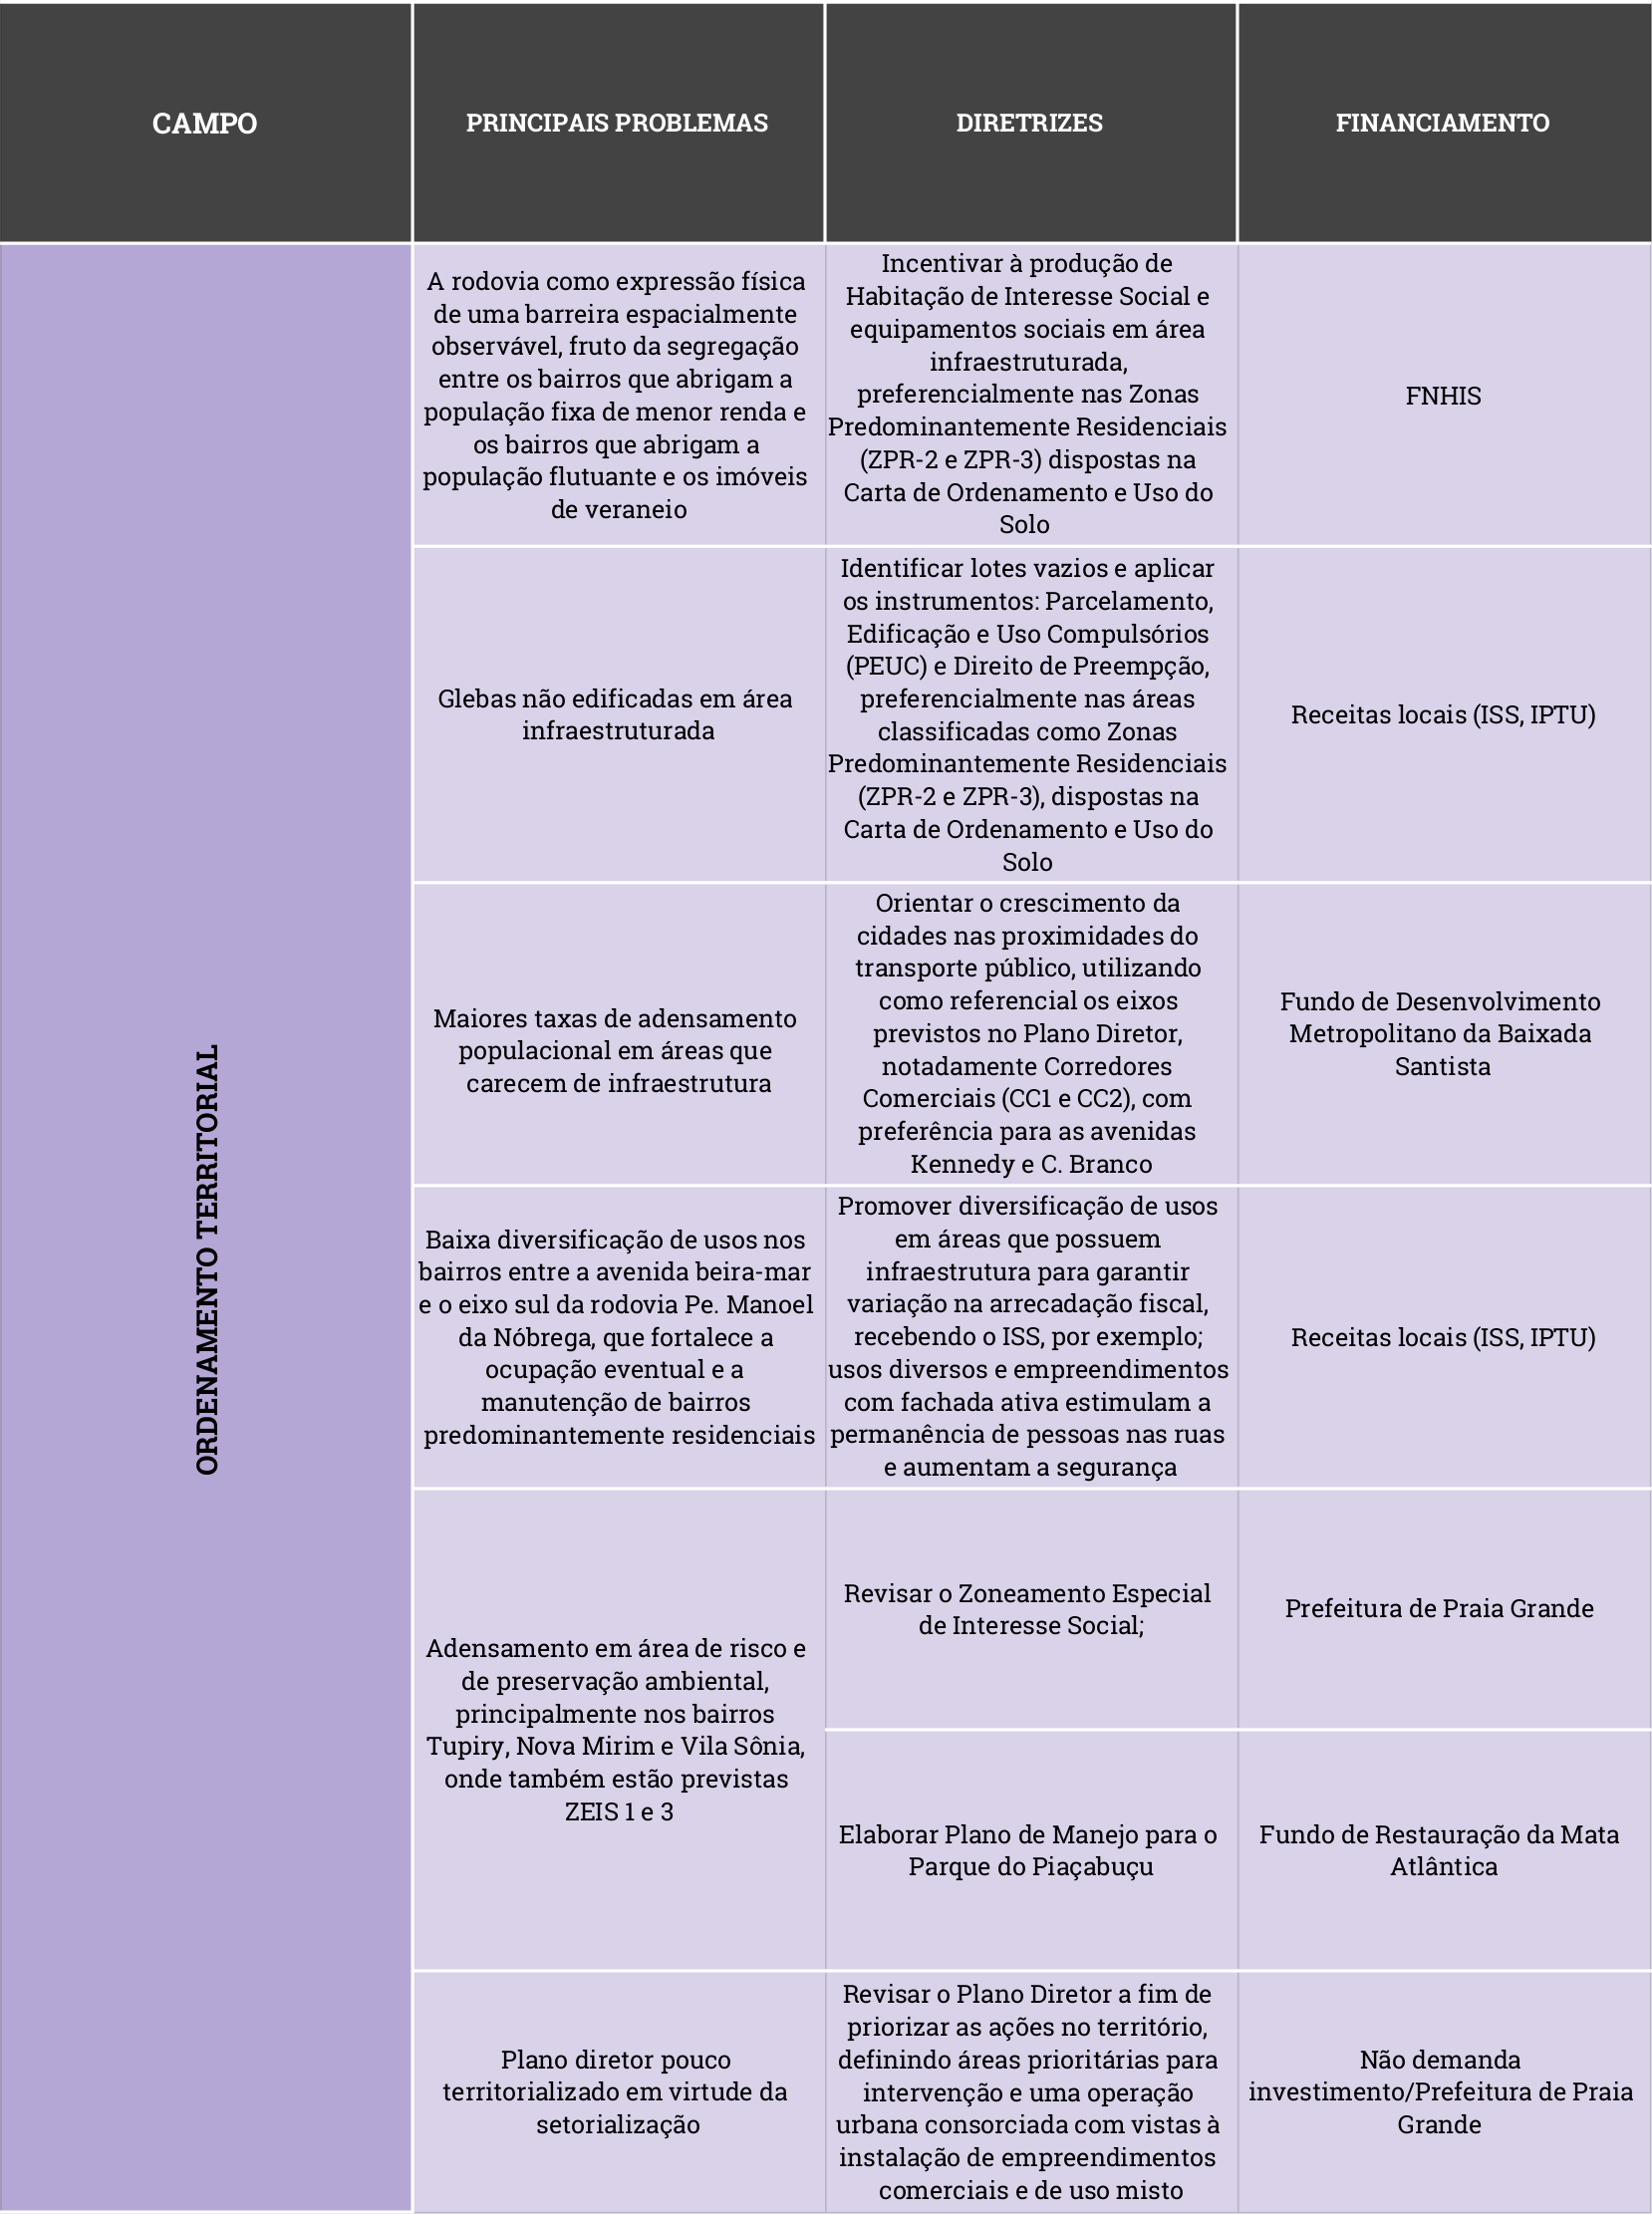
\includegraphics[width=22cm,height=22cm,keepaspectratio]{img/dir01.png}
		\legend{Elaboração própria}
	\end{figure}

	\begin{figure}[h]
		\centering
		\caption{Quadro-síntese de Diretrizes, parte 2}
		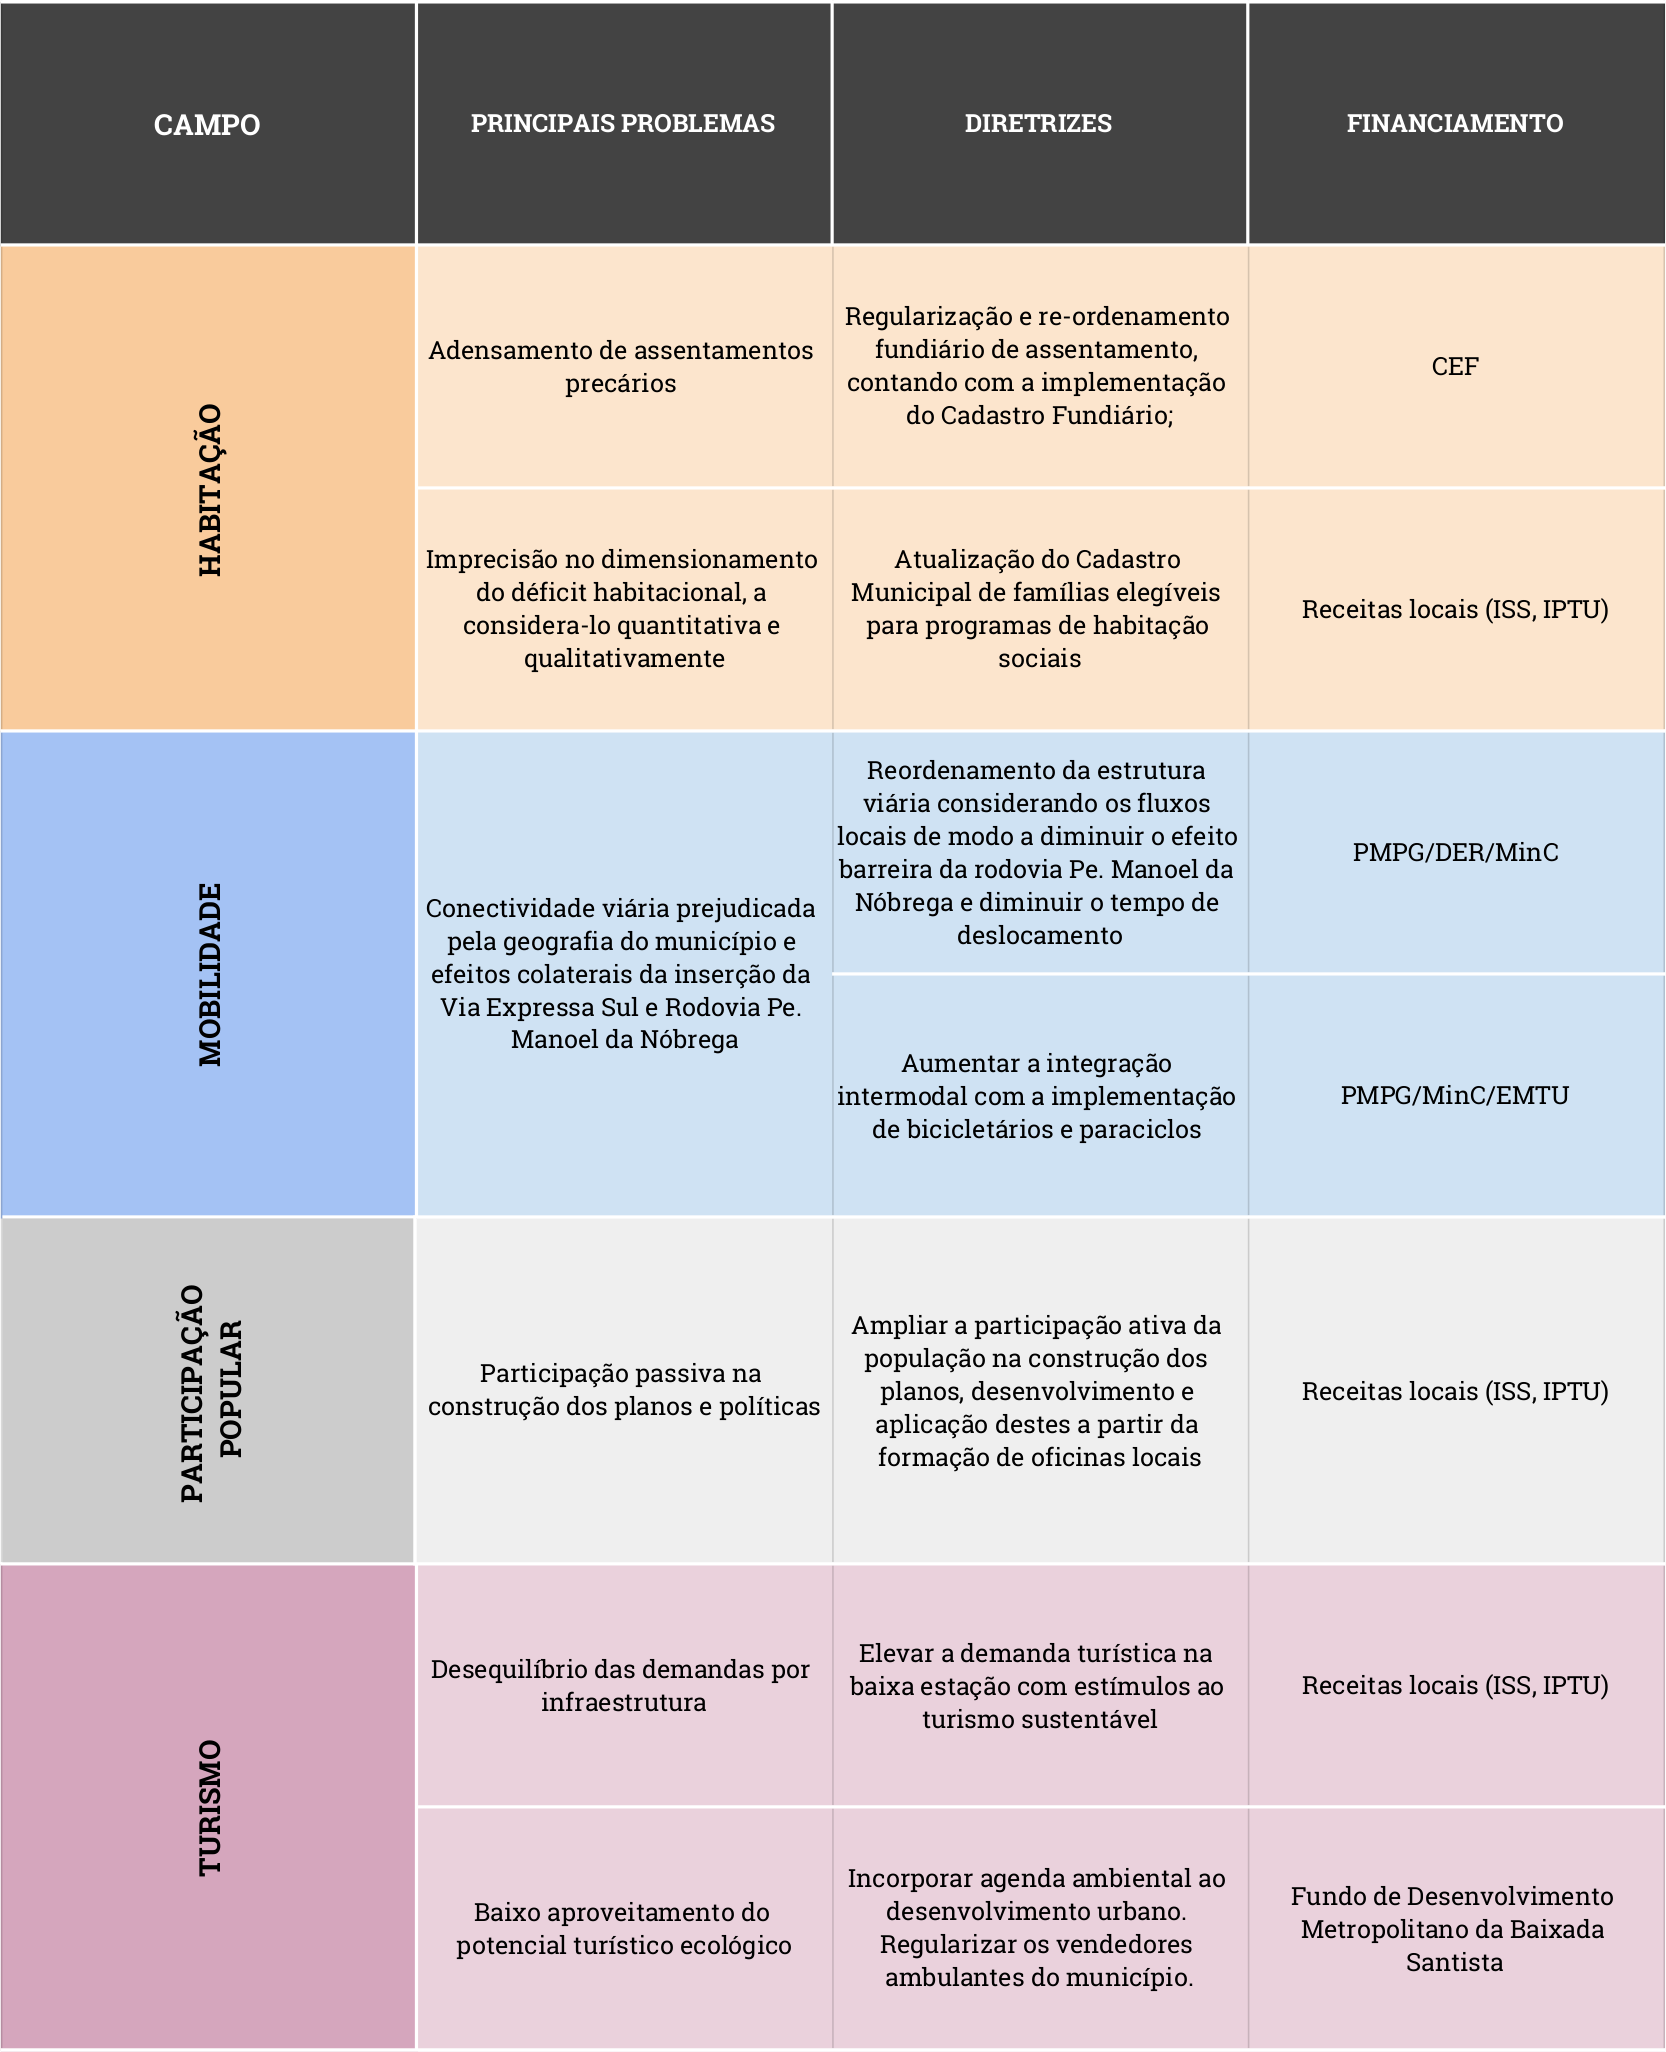
\includegraphics[width=22cm,height=20cm,keepaspectratio]{img/dir02.png}
		\legend{Elaboração própria}
	\end{figure}
    
	\begin{figure}[h]
		\centering
		\caption{Quadro-síntese de Diretrizes, parte 3}
		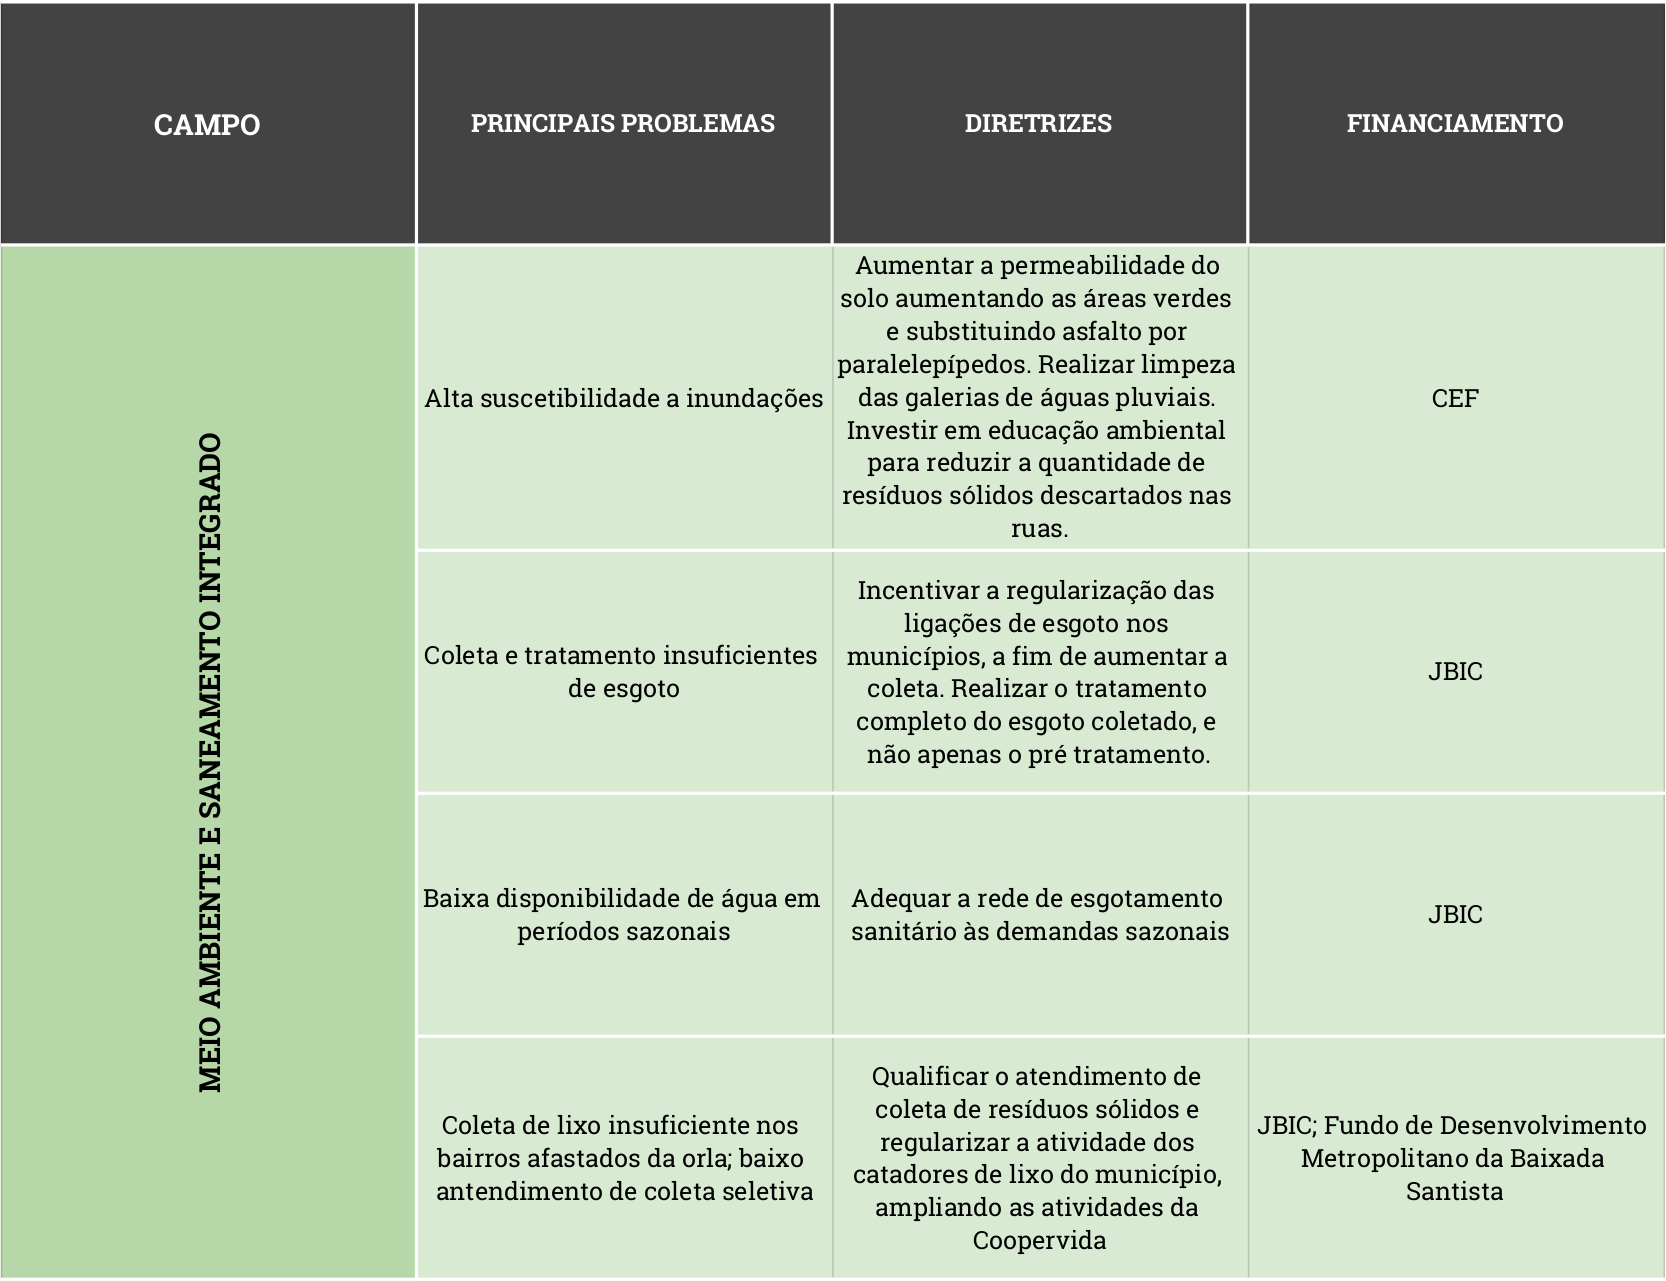
\includegraphics[width=22cm,height=12.4cm,keepaspectratio]{img/dir03.png}
		\legend{Elaboração própria}
	\end{figure}

	\begin{landscape}
		\begin{figure}[h]
			\centering
			\caption{Mapa Síntese das Diretrizes}
			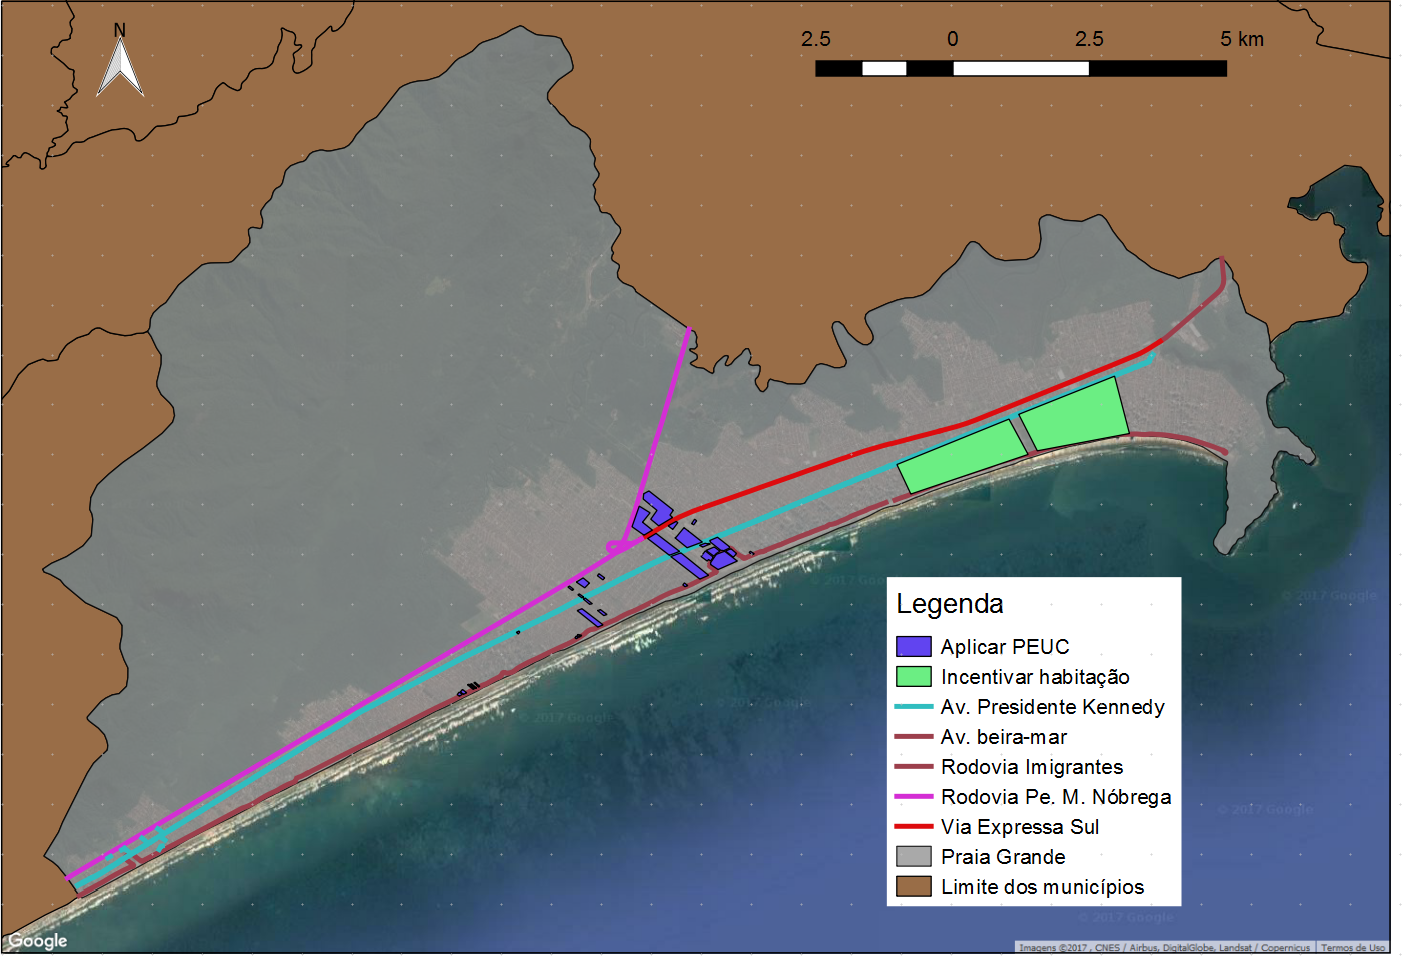
\includegraphics[width=22cm,height=22cm,keepaspectratio]{img/mapa_sintese_diag.png}
			\label{mapa_sintese_diag}
			\legend{Elaboração própria}
		\end{figure}
	\end{landscape}
    
%
%===============================================================================
%

	% ----------------------------------------------------------
	% ----------------------------------------------------------
	\postextual
	
	
	
	% informa o arquivo com a bibliografia. Deve ser o mesmo nome
	% (sem o sufixo) que será informado no ambiente filecontents
	% que está no final deste arquivo. Neste exemplo foi usado 
	% bibitemp.bib e bibtemp. Este comando insere a bibliografia
	% nesta posição (antes dos apêndices, anexos, índice remissivo)
	\bibliography{fontes}
	% ----------------------------------------------------------
	% Glossário
	% ----------------------------------------------------------
	% Consultar manual da classe abntex2 para orientações sobre o
	% uso do glossário.
	\renewcommand{\glossaryname}{Glossário}
	%\renewcommand{\glossarypreamble}{Esta é a descrição do glossário.\\ \\}
	\renewcommand*{\glsseeformat}[3][\seename]{\textit{#1}
		\glsseelist{#2}}
	
	% ---
	% Traduções para o ambiente glossaries
	% ---
	\providetranslation{Glossary}{Glossário}
	\providetranslation{Acronyms}{Siglas}
	\providetranslation{Notation (glossaries)}{Notação}
	\providetranslation{Description (glossaries)}{Descrição}
	\providetranslation{Symbol (glossaries)}{Símbolo}
	\providetranslation{Page List (glossaries)}{Lista de Páginas}
	\providetranslation{Symbols (glossaries)}{Símbolos}
	\providetranslation{Numbers (glossaries)}{Números} 
	% ---
	
	% ---
	% Imprime o glossário
	% ---
	\cleardoublepage
	\phantomsection
	\addcontentsline{toc}{chapter}{\glossaryname}
	% \glossarystyle{index}
	% \glossarystyle{altlisthypergroup}
	\glossarystyle{tree}
	\printglossaries
	% ---
	
	% ----------------------------------------------------------
	% Apêndices
	% ----------------------------------------------------------
	
	% ---
	% Inicia os apêndices. Não esquecer de fechar ao final de
	% todos os apêndices (\end{apendicesenv})
	% ---
	%\begin{apendicesenv}
	
	% Imprime uma página indicando o início dos apêndices
	%\partapendices
	
	% ----------------------------------------------------------
	%\chapter{Primeiro apêndice}
	% ----------------------------------------------------------
	
	%Este é um exemplo de inclusão de capítulos de %apêndice em uma 
	%monografia.  Cada apêndice é tratado como se fosse %um capítulo.
	%Os apêndices devem ser iniciados pelo comando de %ambiente
	%\textbackslash begin\{apendicesenv\} e encerrados %pelo comando 
	%\textbackslash end\{apendicesenv\}.
	
	% ----------------------------------------------------------
	%\chapter{Segundo apêndice}
	% ----------------------------------------------------------
	
	%Este é um exemplo de inclusão de um segundo apêndice. 
	
	%\end{apendicesenv}
	% ---
	
	
	% ----------------------------------------------------------
	% Anexos
	% ----------------------------------------------------------
	
	% ---
	% Inicia os anexos
	% ---
	%\begin{anexosenv}
	
	% Imprime uma página indicando o início dos anexos
	%\partanexos
	
	% ---
	%\chapter{Primeiro anexo}
	% ---
	%Os anexos são similares aos apêndices se distinguindo pelo fato
	%que os apêndices são de autoria do autor da monografia e os 
	%anexos não são da autoria do autor da monografia.  Por exemplo,
	%se incluir no trabalho um modelo de um formulário preenchido
	%por alunos participantes de uma pesquisa, este será um apêndice
	%se o formulário foi criado pelo autor da monografia e será um
	%anexo se o formulário tiver sido criado por outros (por exemplo,
	%é um formulário padrão da escola em que o aluno que o preenche
	%estuda).
	%
	%Mesmo que o formulário tenha sido elaborado pela escola, uma
	%reprodução do formulário preenchido por cada aluno na pesquisa
	%será incluído no apêndice pois envolve o trabalho do autor da
	%monografia ao distribuir, coletar e reproduzir as respostas.
	%
	%Este é um exemplo de inclusão de capítulos de anexos em uma 
	%monografia.  Cada anexo é tratado como se fosse um capítulo.
	%Os anexos devem ser iniciados pelo comando de ambiente
	%\textbackslash begin\{anexoenv\} e encerrados pelo comando 
	%\textbackslash end\{anexoenv\}.
	%
	%\end{anexosenv}
	% ---
	%---------------------------------------------------------------------
	%---------------------------------------------------------------------
	
	%\printindex
	
	% Por padrão são incluídas no trabalho somente as referências
	% citadas ao longo do texto. No comando abaixo foram acrescentadas
	% algumas referências não citadas (neste texto servem apenas como
	% exemplos). Não deve ser usado o comando (mais simples) 
	% \nocite{*}, pois este parece não ser compatível com o
	% abntex2cite
	%\nocite{abntex2cite,abntex2wiki,boyer,eves,iezzi,kletenic,
	%        diomara,steinbruch,intusolatex,feynman,shannon,
	%        luisfelipe,turing}
\end{document}
